% Options for packages loaded elsewhere
\PassOptionsToPackage{unicode}{hyperref}
\PassOptionsToPackage{hyphens}{url}
%
\documentclass[
]{book}
\usepackage{lmodern}
\usepackage{amssymb,amsmath}
\usepackage{ifxetex,ifluatex}
\ifnum 0\ifxetex 1\fi\ifluatex 1\fi=0 % if pdftex
  \usepackage[T1]{fontenc}
  \usepackage[utf8]{inputenc}
  \usepackage{textcomp} % provide euro and other symbols
\else % if luatex or xetex
  \usepackage{unicode-math}
  \defaultfontfeatures{Scale=MatchLowercase}
  \defaultfontfeatures[\rmfamily]{Ligatures=TeX,Scale=1}
\fi
% Use upquote if available, for straight quotes in verbatim environments
\IfFileExists{upquote.sty}{\usepackage{upquote}}{}
\IfFileExists{microtype.sty}{% use microtype if available
  \usepackage[]{microtype}
  \UseMicrotypeSet[protrusion]{basicmath} % disable protrusion for tt fonts
}{}
\makeatletter
\@ifundefined{KOMAClassName}{% if non-KOMA class
  \IfFileExists{parskip.sty}{%
    \usepackage{parskip}
  }{% else
    \setlength{\parindent}{0pt}
    \setlength{\parskip}{6pt plus 2pt minus 1pt}}
}{% if KOMA class
  \KOMAoptions{parskip=half}}
\makeatother
\usepackage{xcolor}
\IfFileExists{xurl.sty}{\usepackage{xurl}}{} % add URL line breaks if available
\IfFileExists{bookmark.sty}{\usepackage{bookmark}}{\usepackage{hyperref}}
\hypersetup{
  pdftitle={The BOAST Style Guide},
  pdfauthor={Neil Hatfield (njh5464@psu.edu) and Robert Carey (rpc5102@psu.edu)},
  hidelinks,
  pdfcreator={LaTeX via pandoc}}
\urlstyle{same} % disable monospaced font for URLs
\usepackage{color}
\usepackage{fancyvrb}
\newcommand{\VerbBar}{|}
\newcommand{\VERB}{\Verb[commandchars=\\\{\}]}
\DefineVerbatimEnvironment{Highlighting}{Verbatim}{commandchars=\\\{\}}
% Add ',fontsize=\small' for more characters per line
\usepackage{framed}
\definecolor{shadecolor}{RGB}{248,248,248}
\newenvironment{Shaded}{\begin{snugshade}}{\end{snugshade}}
\newcommand{\AlertTok}[1]{\textcolor[rgb]{0.94,0.16,0.16}{#1}}
\newcommand{\AnnotationTok}[1]{\textcolor[rgb]{0.56,0.35,0.01}{\textbf{\textit{#1}}}}
\newcommand{\AttributeTok}[1]{\textcolor[rgb]{0.77,0.63,0.00}{#1}}
\newcommand{\BaseNTok}[1]{\textcolor[rgb]{0.00,0.00,0.81}{#1}}
\newcommand{\BuiltInTok}[1]{#1}
\newcommand{\CharTok}[1]{\textcolor[rgb]{0.31,0.60,0.02}{#1}}
\newcommand{\CommentTok}[1]{\textcolor[rgb]{0.56,0.35,0.01}{\textit{#1}}}
\newcommand{\CommentVarTok}[1]{\textcolor[rgb]{0.56,0.35,0.01}{\textbf{\textit{#1}}}}
\newcommand{\ConstantTok}[1]{\textcolor[rgb]{0.00,0.00,0.00}{#1}}
\newcommand{\ControlFlowTok}[1]{\textcolor[rgb]{0.13,0.29,0.53}{\textbf{#1}}}
\newcommand{\DataTypeTok}[1]{\textcolor[rgb]{0.13,0.29,0.53}{#1}}
\newcommand{\DecValTok}[1]{\textcolor[rgb]{0.00,0.00,0.81}{#1}}
\newcommand{\DocumentationTok}[1]{\textcolor[rgb]{0.56,0.35,0.01}{\textbf{\textit{#1}}}}
\newcommand{\ErrorTok}[1]{\textcolor[rgb]{0.64,0.00,0.00}{\textbf{#1}}}
\newcommand{\ExtensionTok}[1]{#1}
\newcommand{\FloatTok}[1]{\textcolor[rgb]{0.00,0.00,0.81}{#1}}
\newcommand{\FunctionTok}[1]{\textcolor[rgb]{0.00,0.00,0.00}{#1}}
\newcommand{\ImportTok}[1]{#1}
\newcommand{\InformationTok}[1]{\textcolor[rgb]{0.56,0.35,0.01}{\textbf{\textit{#1}}}}
\newcommand{\KeywordTok}[1]{\textcolor[rgb]{0.13,0.29,0.53}{\textbf{#1}}}
\newcommand{\NormalTok}[1]{#1}
\newcommand{\OperatorTok}[1]{\textcolor[rgb]{0.81,0.36,0.00}{\textbf{#1}}}
\newcommand{\OtherTok}[1]{\textcolor[rgb]{0.56,0.35,0.01}{#1}}
\newcommand{\PreprocessorTok}[1]{\textcolor[rgb]{0.56,0.35,0.01}{\textit{#1}}}
\newcommand{\RegionMarkerTok}[1]{#1}
\newcommand{\SpecialCharTok}[1]{\textcolor[rgb]{0.00,0.00,0.00}{#1}}
\newcommand{\SpecialStringTok}[1]{\textcolor[rgb]{0.31,0.60,0.02}{#1}}
\newcommand{\StringTok}[1]{\textcolor[rgb]{0.31,0.60,0.02}{#1}}
\newcommand{\VariableTok}[1]{\textcolor[rgb]{0.00,0.00,0.00}{#1}}
\newcommand{\VerbatimStringTok}[1]{\textcolor[rgb]{0.31,0.60,0.02}{#1}}
\newcommand{\WarningTok}[1]{\textcolor[rgb]{0.56,0.35,0.01}{\textbf{\textit{#1}}}}
\usepackage{longtable,booktabs}
% Correct order of tables after \paragraph or \subparagraph
\usepackage{etoolbox}
\makeatletter
\patchcmd\longtable{\par}{\if@noskipsec\mbox{}\fi\par}{}{}
\makeatother
% Allow footnotes in longtable head/foot
\IfFileExists{footnotehyper.sty}{\usepackage{footnotehyper}}{\usepackage{footnote}}
\makesavenoteenv{longtable}
\usepackage{graphicx,grffile}
\makeatletter
\def\maxwidth{\ifdim\Gin@nat@width>\linewidth\linewidth\else\Gin@nat@width\fi}
\def\maxheight{\ifdim\Gin@nat@height>\textheight\textheight\else\Gin@nat@height\fi}
\makeatother
% Scale images if necessary, so that they will not overflow the page
% margins by default, and it is still possible to overwrite the defaults
% using explicit options in \includegraphics[width, height, ...]{}
\setkeys{Gin}{width=\maxwidth,height=\maxheight,keepaspectratio}
% Set default figure placement to htbp
\makeatletter
\def\fps@figure{htbp}
\makeatother
\setlength{\emergencystretch}{3em} % prevent overfull lines
\providecommand{\tightlist}{%
  \setlength{\itemsep}{0pt}\setlength{\parskip}{0pt}}
\setcounter{secnumdepth}{5}
\usepackage{booktabs}
\usepackage{amsthm}
\makeatletter
\def\thm@space@setup{%
  \thm@preskip=8pt plus 2pt minus 4pt
  \thm@postskip=\thm@preskip
}
\makeatother
\usepackage[]{natbib}
\bibliographystyle{apalike}

\title{The BOAST Style Guide}
\author{Neil Hatfield (\href{mailto:njh5464@psu.edu}{\nolinkurl{njh5464@psu.edu}}) and Robert Carey (\href{mailto:rpc5102@psu.edu}{\nolinkurl{rpc5102@psu.edu}})}
\date{04 June 2020}

\begin{document}
\maketitle

{
\setcounter{tocdepth}{1}
\tableofcontents
}
\hypertarget{welcome}{%
\chapter*{Welcome}\label{welcome}}
\addcontentsline{toc}{chapter}{Welcome}

This guide spells out the styling that should be used for all apps included in the \href{https://github.com/EducationShinyAppTeam/BOAST}{Book of Apps for Statistics Teaching (BOAST)}.

There are several different aspects to what makes up styling including:

\begin{itemize}
\tightlist
\item
  Coding (how you write, organize, and comment the code that makes the app)
\item
  Visual Appearance (how you make the app look including tabs, fonts, colors, icons, etc.)
\item
  Wording (how you write information, instructions, and other messages to the users)
\item
  Documentation (how you provide references, including code and data sources, and give credit)
\end{itemize}

In addition to these elements, we've provide information on ensuring that your App is accessible to all users and works well on mobile devices such as smart phones and tablets.

Whenever possible, we've attempted to provide you with examples to help you see our standards in action as well as code that you can use as templates. For each code block, you should be able to place your cursor over the block and see a copy icon in the upper-right hand corner. This will allow you to copy the code. We've also included links to additional resources so that you can learn more about key topics.

You will need to follow this Style Guide to ensure that any app you create meets (or exceeds) our standards is worth of inclusion in BOAST.

This Style Guide is laid out in several parts:

\begin{itemize}
\tightlist
\item
  Part 1 covers the basics for getting started
\item
  Part 2 focuses on Coding Style
\item
  Part 3 deals with the many aspects of Visual Styling
\item
  Part 4 centers on Linguistic Styling
\item
  Part 5 conveys important information on Accessibility and Mobile Friendliness
\item
  Part 6 is where you can see an example of building an app from scratch
\item
  The final part is where you can find some additional tools and information.
\end{itemize}

\hypertarget{part-getting-started}{%
\part{Getting Started}\label{part-getting-started}}

\setcounter{chapter}{0}

\hypertarget{basics}{%
\chapter{The Basics}\label{basics}}

Before you get too far into the Style Guide, we would like for you to take a moment and ensure that you have the following tools at your disposal.

\hypertarget{checklist}{%
\section{Getting Started Checklist}\label{checklist}}

\begin{enumerate}
\def\labelenumi{\arabic{enumi}.}
\item
  Ensure that you have all of necessary accounts and if not, put in a request to Bob (\href{mailto:rpc5102@psu.edu}{rpc5102}).

  \begin{enumerate}
  \def\labelenumii{\alph{enumii}.}
  \tightlist
  \item
    \href{https://www.datacamp.com/}{DataCamp}\\
  \item
    \href{https://github.com/}{GitHub}\\
  \item
    \href{https://github.com/EducationShinyAppTeam}{EducationShinyAppTeam}
  \item
    \href{https://teams.microsoft.com/l/team/19\%3a8423bc25992a4451952d8312b497324d\%40thread.skype/conversations?groupId=a83c9d1b-6bcc-46f4-aa25-82b2fad862ec\&tenantId=7cf48d45-3ddb-4389-a9c1-c115526eb52e}{BOAST} in Microsoft Teams (tied to your PSU AccessID)
  \end{enumerate}
\item
  Ensure that you have all of the required software

  \begin{enumerate}
  \def\labelenumii{\alph{enumii}.}
  \tightlist
  \item
    \href{https://cloud.r-project.org/}{\texttt{R} (version 3.5.* minimum, version 4.0.0 preferred)}
  \item
    \href{https://rstudio.com/products/rstudio/download/\#download}{RStudio Desktop (most current version preferred)}
  \end{enumerate}
\item
  Additional Software that we strongly recommend

  \begin{enumerate}
  \def\labelenumii{\alph{enumii}.}
  \tightlist
  \item
    \href{https://desktop.github.com/}{GitHub Desktop}{]}
  \end{enumerate}
\item
  \texttt{R} Packages--here are some basic packages that everyone will need; be sure to install their dependencies

\begin{Shaded}
\begin{Highlighting}[]
\KeywordTok{install.packages}\NormalTok{(}\KeywordTok{c}\NormalTok{(}\StringTok{"devtools"}\NormalTok{, }\StringTok{"DT"}\NormalTok{, }\StringTok{"ggplot2"}\NormalTok{, }\StringTok{"shiny"}\NormalTok{, }\StringTok{"shinyBS"}\NormalTok{, }
                   \StringTok{"shinyWidgets"}\NormalTok{, }\StringTok{"tidyverse"}\NormalTok{, }\StringTok{"tippy"}\NormalTok{))}
\end{Highlighting}
\end{Shaded}
\item
  A copy of the Sample App (\protect\hyperlink{sample-app}{see below})
\end{enumerate}

\hypertarget{boastutils-package}{%
\section{\texorpdfstring{\texttt{boastUtils} Package}{boastUtils Package}}\label{boastutils-package}}

Bob created the \href{https://github.com/EducationShinyAppTeam/boastUtils}{boastUtils} package to automate much of the design and development process. This will not only reduce the amount of work you'll need to do, it'll also make apps more consistent.

\textbf{Starting Summer 2020, you will be required to you make use of this tool.}

Please check out the \href{https://github.com/EducationShinyAppTeam/boastUtils}{package's GitHub page} for instructions on installing and usage.

\begin{Shaded}
\begin{Highlighting}[]
\KeywordTok{library}\NormalTok{(devtools)}
\NormalTok{devtools}\OperatorTok{::}\KeywordTok{install_github}\NormalTok{(}\StringTok{"EducationShinyAppTeam/boastUtils"}\NormalTok{)}
\end{Highlighting}
\end{Shaded}

\hypertarget{sample-app}{%
\section{Sample App}\label{sample-app}}

Bob and Neil have created a Sample App repository that you can use as a template for your own apps. To get started, clone the \href{https://github.com/EducationShinyAppTeam/Sample_App}{Sample\_App} template repo found on GitHub. This will provide you with a skeleton for organizing your files as well as your code.

There are several methods you can use:

\begin{itemize}
\tightlist
\item
  \protect\hyperlink{direct-download}{Direct Download (Basic)}
\item
  \protect\hyperlink{github-desktop}{GitHub Desktop (Recommended)}
\item
  \protect\hyperlink{command-line}{Command Line (Advanced)}
\item
  \protect\hyperlink{rstudio-project}{RStudio Project}
\end{itemize}

\hypertarget{direct-download}{%
\subsection{Direct Download}\label{direct-download}}

You can download this repository directly by visiting:

\begin{quote}
\url{https://github.com/EducationShinyAppTeam/Sample_App/archive/master.zip}
\end{quote}

\hypertarget{github-desktop}{%
\subsection{GitHub Desktop}\label{github-desktop}}

If you are using \href{https://desktop.github.com/}{GitHub Desktop} and have \href{https://help.github.com/en/desktop/getting-started-with-github-desktop/authenticating-to-github}{linked your account} that has access to the \href{https://github.com/EducationShinyAppTeam}{EducationShinyAppTeam} repository, you can do the following from inside GitHub Desktop:

\begin{enumerate}
\def\labelenumi{\arabic{enumi}.}
\tightlist
\item
  Bring up the Clone Repository Menu (File -\textgreater{} Clone Repository\ldots)\\
\item
  Enter Sample\_App in the search bar and select the option that says Sample\_App (not sampleapp)
\item
  Click the Choose\ldots{} button for the local path (this is where you want to the clone to live on your computer)
\item
  Click the Clone button.
\end{enumerate}

\textbf{See also:}

\begin{itemize}
\tightlist
\item
  \href{https://help.github.com/en/desktop}{GitHub Desktop Help}
\end{itemize}

\hypertarget{command-line}{%
\subsection{Command Line}\label{command-line}}

Enter the following command in your terminal:

\begin{Shaded}
\begin{Highlighting}[]
\FunctionTok{git}\NormalTok{ clone git@github.com:EducationShinyAppTeam/Sample_App.git}
\end{Highlighting}
\end{Shaded}

\textbf{See also:}

\begin{itemize}
\tightlist
\item
  \href{https://guides.github.com/introduction/git-handbook/}{Git Handbook}
\item
  \href{https://try.github.io/}{Resources to learn Git}
\item
  \href{https://happygitwithr.com/}{Happy Git and GitHub for the userR}
\end{itemize}

\hypertarget{rstudio-project}{%
\subsection{RStudio Project}\label{rstudio-project}}

You can also use RStudio to connect to and copy repositories from GitHub. There are a few extra steps that you'll need to go through compared to other methods. We recommend that you use GitHub Desktop.

\begin{enumerate}
\def\labelenumi{\arabic{enumi}.}
\tightlist
\item
  In your browser, navigate to the repository you want to copy; in this case the \href{https://github.com/EducationShinyAppTeam/Sample_App}{Sample\_App repo}.
\item
  Launch RStudio and create a new project.
\item
  Select the Version Control option and then Git.
\item
  Switch back to your browser and click on the Clone or Download button. There should be a line of text starting with \texttt{git@github} that you can copy. Do so.
\item
  Returning to RStudio, paste the get you just copied into the Repository URL field.
\item
  Adjust the directory name and the subdirectory (where this project will live on your machine) as you see fit.
\item
  Click the Create Project button.
\end{enumerate}

This method will ensure that you will be able to successfully push and pull changes to GitHub. For additional help, Neil has created a video ``\href{https://youtu.be/IK0SiEz5vjs}{Using RStudio to Connect to GitHub}'' which walks you through the process.

\hypertarget{workflow}{%
\chapter{Workflow}\label{workflow}}

As you work on apps, both updating existing and developing new ones, moving through a workflow can help you organize yourself.

\hypertarget{revising-existing-apps}{%
\section{Revising Existing Apps}\label{revising-existing-apps}}

\begin{enumerate}
\def\labelenumi{\arabic{enumi}.}
\tightlist
\item
  Read the Style Guide
\item
  Explore the existing apps in the \href{https://sites.psu.edu/shinyapps/}{book}
\item
  When you identify an app you wish to work on,

  \begin{enumerate}
  \def\labelenumii{\alph{enumii}.}
  \tightlist
  \item
    Go to that app's repository in \href{https://github.com/EducationShinyAppTeam}{GitHub}
  \item
    Create new issues on GitHub to log both bugs and suggestions for improvements
  \item
    Create an issue specifically if the App currently does not abide by this Style Guide
  \item
    Optional--assign yourself to the issue
  \end{enumerate}
\item
  Download the current version of the app by using either RStudio or GitHub Desktop.
\item
  Create a new branch for your developments.
\item
  Begin editing the code
\item
  As you edit, be sure to reference this Style Guide and test your code locally via Run App in RStudio.
\item
  Periodically push your edits to your development branch. Don't forget to add commit messages and reference any issues.
\item
  When you're ready to do larger scale testing you'll need to publish your App to the TLT RStudio Connect server (see \protect\hyperlink{testing}{Section \ref{testing}}).
\item
  When you've reached a point where you've finished editing, push your most recent commit to your development branch and then create a Pull Request. Assign Neil as a reviewer.
\item
  Make any requested changes and re-push to your development branch. Update the Pull Request with a new comment.
\end{enumerate}

If everything checks out, then we'll merge your development branch with the master branch and schedule formal deployment of your App.

\hypertarget{creating-new-apps}{%
\section{Creating New Apps}\label{creating-new-apps}}

To see this workflow in action, check out \protect\hyperlink{makingApp}{Chapter \ref{makingApp}}.

\begin{enumerate}
\def\labelenumi{\arabic{enumi}.}
\tightlist
\item
  Read the Style Guide
\item
  Identify a topic for your new App
\item
  Sketch out your plans for the App. \textbf{This should occur BEFORE you start coding.} Be sure that you include:

  \begin{enumerate}
  \def\labelenumii{\alph{enumii}.}
  \tightlist
  \item
    Suggested Title
  \item
    Goal of the app
  \item
    What will the user be doing (i.e., potential inputs)
  \item
    What will the user be experiencing (i.e., potential outputs)
  \item
    Relationships between various elements.
  \end{enumerate}
\item
  When your plan \textbf{gets approval}, create a new repository on GitHub (see \protect\hyperlink{repo-naming}{Section \ref{repo-naming}}); you can initially load the Sample App template to this repository, if you wish.
\item
  Begin writing the code
\item
  As you edit, be sure to reference this Style Guide and test your code locally via Run App in RStudio.
\item
  When you get the basic structure of your App set up, push your code to GitHub and create a new development branch for your continued editing. You can open new issues on your app as you go.
\item
  Periodically push your edits to your development branch. Don't forget to add commit messages and reference any issues.
\item
  When you're ready to do larger scale testing you'll need to publish your App to the TLT RStudio Connect server (see \protect\hyperlink{testing}{Section \ref{testing}}).
\item
  When you've reached a point where you've finished editing, push your most recent commit to your development branch and then create a Pull Request. Assign Neil as a reviewer.
\item
  Make any requested changes and re-push to your development branch. Update the Pull Request with a new comment.
\end{enumerate}

If everything checks out, then we'll merge your development branch with the master branch and schedule formal deployment of your App.

\hypertarget{repo-naming}{%
\subsection{GitHub Repo Names}\label{repo-naming}}

Each Shiny App has its own repository (repo) on GitHub. As you begin to create new apps, you'll have to create a new repo on GitHub for each one. The name of that repo is extremely important as this will play a critical role in establishing the URL for your App. To this end, you need to adhere to following guidelines:

\begin{itemize}
\tightlist
\item
  Use \href{https://en.wikipedia.org/wiki/Letter_case\#Title_case}{Title Case} (not camelCase)
\item
  Use underscores ( \_ ) instead of spaces
\item
  Match the App name as closely as possible
\item
  You have a 100 character limit
\end{itemize}

While we can change repo names, doing so results in a large number of edits that have to be made. Thus, think carefully about how you are going to name your repository.

If you come across a repo that is poorly named, please make an issue and provide some suggestions for new names.

\hypertarget{testing}{%
\section{Testing Your App}\label{testing}}

To test your App beyond your local machine, we will be making use of TLT's RStudio Connect platform. You will need to following these directions.

\hypertarget{set-uplogin-to-the-vpn}{%
\subsection{Set Up/Login to the VPN}\label{set-uplogin-to-the-vpn}}

Please refer to the following PSU Knowledge Basis Articles:

\begin{itemize}
\tightlist
\item
  \href{https://pennstate.service-now.com/sp?id=kb_article\&sys_id=c628298bdb1d6f44a318fb671d961971}{VPN for Mac OS}
\item
  \href{https://pennstate.service-now.com/sp?id=kb_article_view\&sys_kb_id=c151310cdb85abc84222778ebf961957}{VPN for Windows}
\item
  \href{https://pennstate.service-now.com/sp?id=kb_article_view\&sys_kb_id=1de84eb6dbd5ab44a318fb671d9619a5}{VPN for Apple iOS}
\item
  \href{https://pennstate.service-now.com/sp?id=kb_article_view\&sys_kb_id=a35e0a7edb59ab44a318fb671d961964}{VPN for Android}
\end{itemize}

You MUST be logged into the PSU VPN to both upload and test your App on each device.

\hypertarget{connecting-your-rstudio-to-tlts-rstudio-connect}{%
\subsection{Connecting Your RStudio to TLT's RStudio Connect}\label{connecting-your-rstudio-to-tlts-rstudio-connect}}

You only need to do this step once.

\begin{enumerate}
\def\labelenumi{\arabic{enumi}.}
\tightlist
\item
  After you've logged into the PSU VPN, go to \href{https://rstudio-connect.tlt.psu.edu:3939/connect}{TLT's RStudio Connect} and log in using your PSU ID.
\item
  Once logged in, click on the Publish button as shown in the green box of \protect\hyperlink{fig:testing1}{Figure \ref{fig:testing1}}

  \begin{figure}
  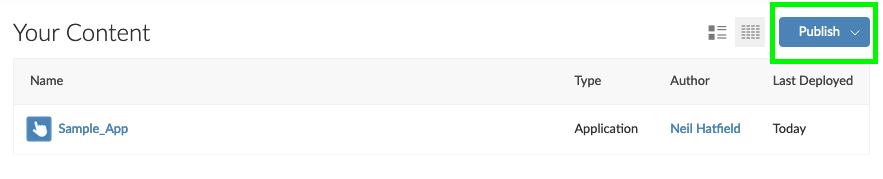
\includegraphics[width=12.26in]{images/publish1} \caption{Click the Publish Button}\label{fig:testing1}
  \end{figure}
\item
  Select Shiny App and a pop up window will appear.
\item
  Follow the steps in this window (especially Step 4) to set up the connection.
\end{enumerate}

\hypertarget{checking-youve-connected}{%
\subsubsection{Checking You've Connected}\label{checking-youve-connected}}

You can check to see if you've connected by going into RStudio's Options and looking at the Publishing tab. You should see a similar entry as what is in the green box of \protect\hyperlink{fig:testing2}{Figure \ref{fig:testing2}}:

\begin{figure}

{\centering 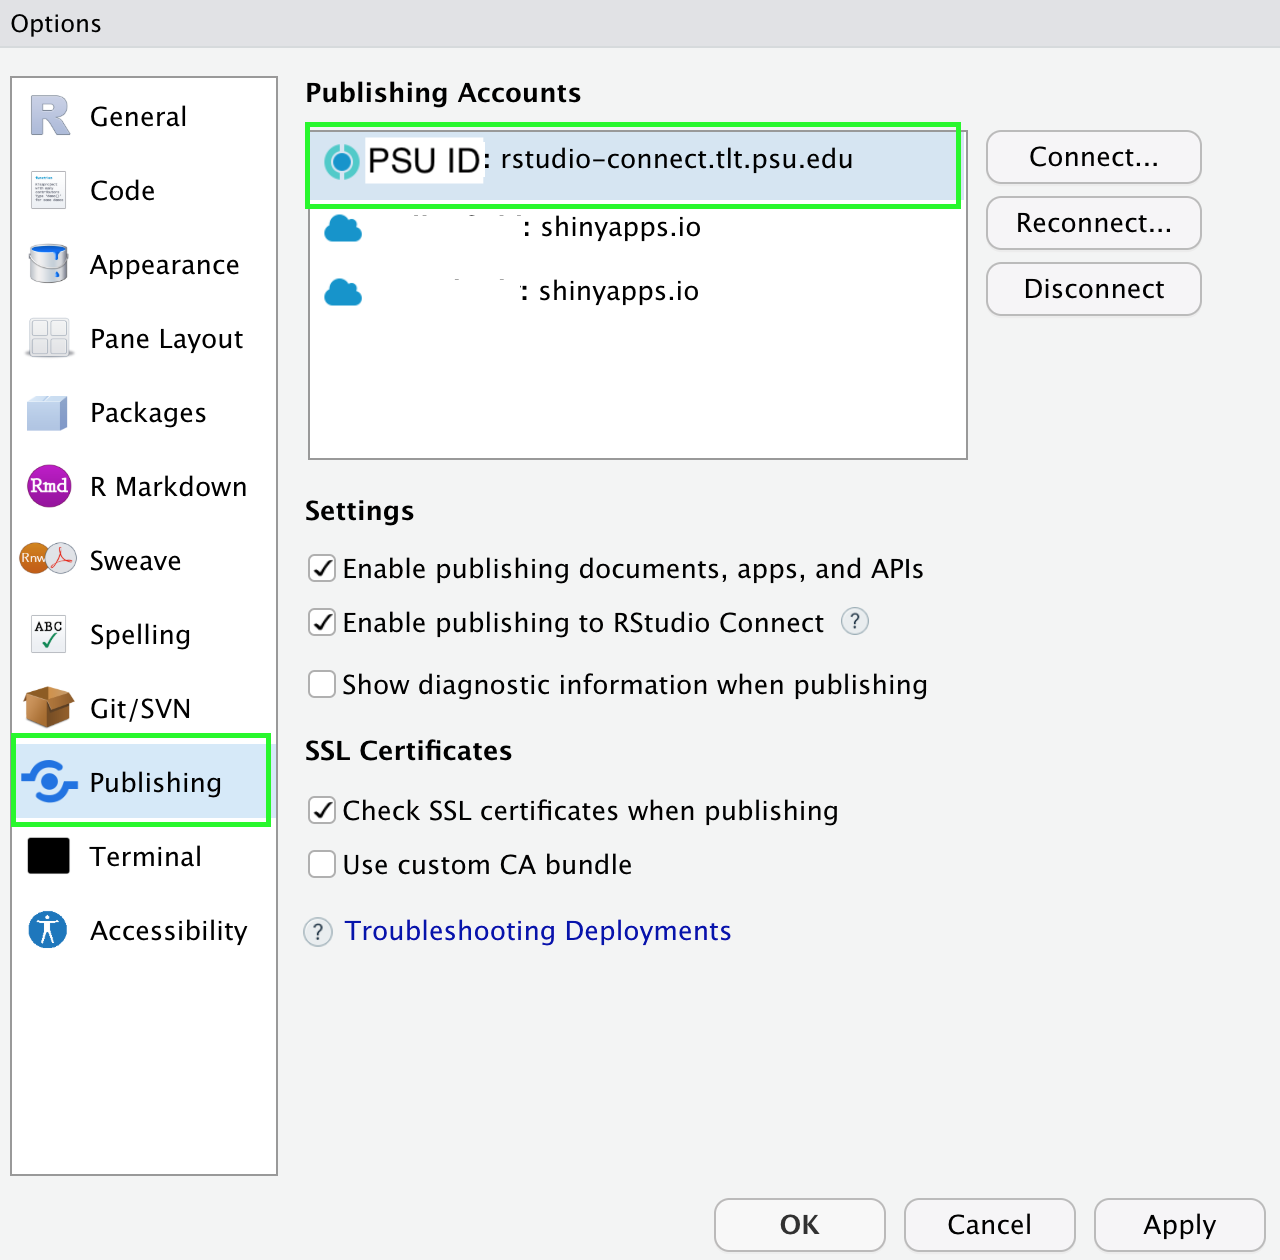
\includegraphics[width=17.78in]{images/publish2} 

}

\caption{Check Your Publishing Profile}\label{fig:testing2}
\end{figure}

\hypertarget{publishing-your-app-for-testing}{%
\subsection{Publishing Your App for Testing}\label{publishing-your-app-for-testing}}

Make sure that you are connected to PSU's VPN and that you've already connected your RStudio to TLT's server.

Click on the Publishing Icon, located just to the right of the Run App button. Be sure to select the TLT Server.

\hypertarget{configuring-for-testing}{%
\subsection{Configuring for Testing}\label{configuring-for-testing}}

Once your App has been published, a new window should open in your browser that shows your App plus the optional controls.

\begin{figure}

{\centering 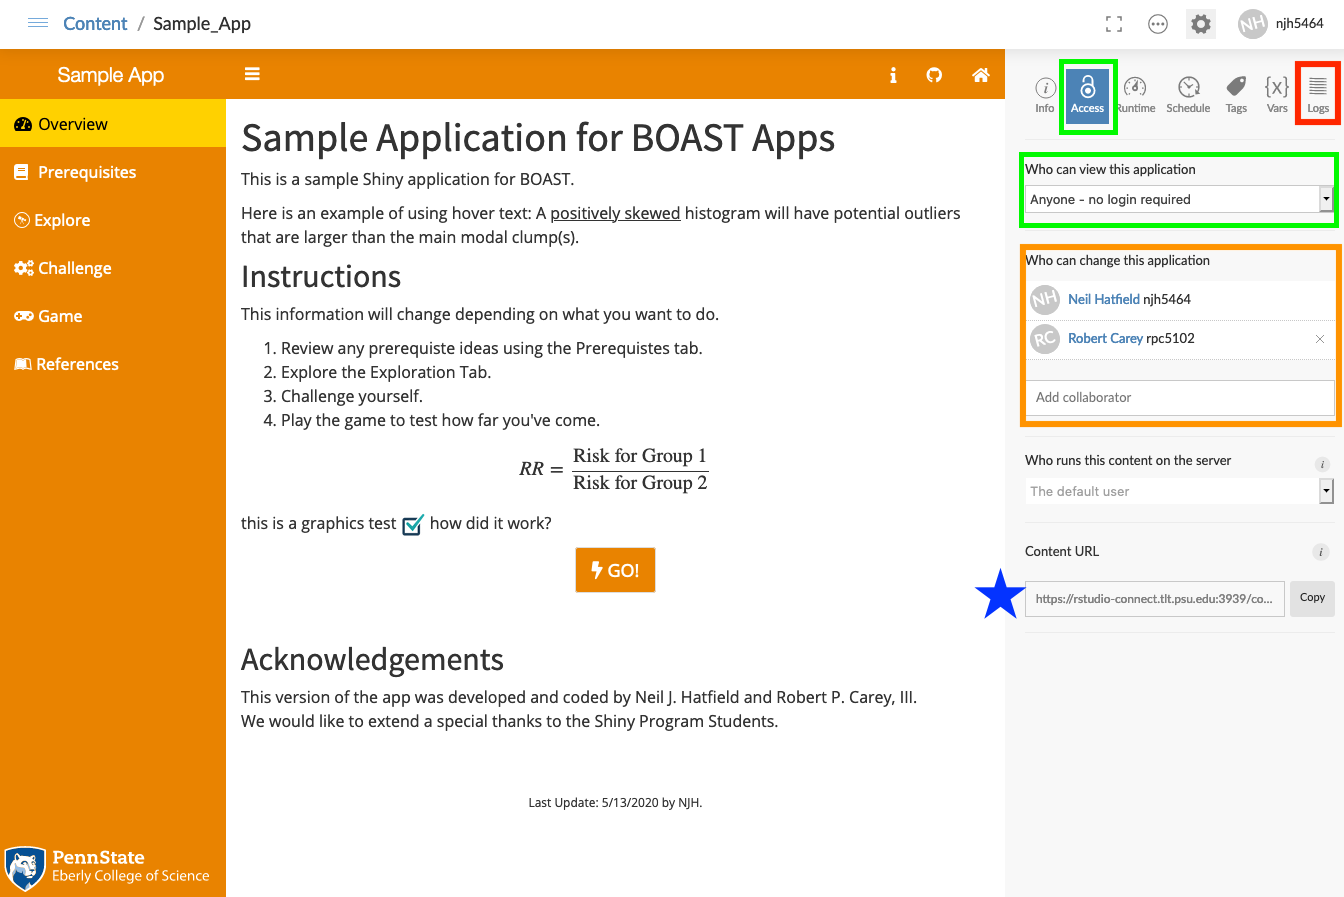
\includegraphics[width=18.67in]{images/publish3} 

}

\caption{Successful Publish and Settings}\label{fig:testing3}
\end{figure}

In \protect\hyperlink{fig:testing3}{Figure \ref{fig:testing3}}, you will need to change a setting to enable others (people and devices) to test your app. Click on the Access tab and set Who can view this application to Anyone-no login required. (These are highlighted in the green boxes.) Keep in mind that all users/devices MUST first connect to the PSU VPN to access your app.

If you want, you can add collaborators as I did in the example (orange box). This is not required.

The most important piece is the Content URL (marked with the blue star). You'll need to copy this URL and give that URL out to your testers. This will allow them easily access your app, regardless of the type of device they are using.

\hypertarget{check-the-logs}{%
\subsection{Check the Logs}\label{check-the-logs}}

As you test your App, you'll want to look for any error messages and/or warnings that get generated. Click on the Logs tab (red box in \protect\hyperlink{fig:testing3}{Figure \ref{fig:testing3}}) to view.

\hypertarget{problems}{%
\subsection{Problems?}\label{problems}}

If you run into problem either publishing your App or getting the App to launch on the TLT, please reach out to Neil and Bob.

\hypertarget{part-writing-code}{%
\part{Writing Code}\label{part-writing-code}}

\hypertarget{coding}{%
\chapter{Coding Style}\label{coding}}

Now that you've gone through the Getting Started section, we can turn our attention to the first part of the Style Guide: Coding. There are many aspects that fall under the heading of Coding Style.

\hypertarget{genCode}{%
\section{General Coding Style}\label{genCode}}

Our general practice is to make use of the \href{https://style.tidyverse.org/}{tidyverse style guide}. However, we do have some important departures and additional practices you need to follow:

\begin{itemize}
\tightlist
\item
  \protect\hyperlink{comments}{Leave comments}
\item
  \protect\hyperlink{naming}{Use informative names}
\item
  \protect\hyperlink{formatCode}{Format your code}
\item
  \protect\hyperlink{explicit}{Be explicit}
\end{itemize}

\hypertarget{comments}{%
\subsection{Leave Comments}\label{comments}}

At bare minimum, use a comment to break your code into sections. This helps you and others conceptualize the code into more manageable chunks. Your comments can provide others with potential keywords to search for when looking at your code later on.

For particularly complex sections, use comments to summarize what you're trying to do. This can help you and others pick up the coding thread for what you are trying to do for troubleshooting, debugging, and future improvements.

\hypertarget{naming}{%
\subsection{Informative Names}\label{naming}}

Use informative names for variables and functions in your code. Use names that give another person a sense of what that variable represents (nouns) or what the function is supposed to do (action verbs). For example,

\begin{itemize}
\tightlist
\item
  \texttt{scoreMatrix} is a matrix that holds a set of scores\\
\item
  \texttt{checkGame} is a function that checks the state of the current game
\end{itemize}

Use \href{https://en.wikipedia.org/wiki/Camel_case}{camelCase} for variable names and functions. The first word begins with a lowercase letter and additional words start with Capital letters with no spaces or underscores ( \_ ) between them. (This is a departure from the tidyverse style.)

Avoid using the variable names from code that you're making use of from another app or script. For example, don't use \texttt{waitTimes} to hold your data on the number of correct answers a user has given. It is also good practice to avoid re-using function names that appear in other libraries that are currently loaded to avoid \href{https://en.wikipedia.org/wiki/Naming_collision}{namespace collision}.

\hypertarget{formatCode}{%
\subsection{Format Your Code}\label{formatCode}}

See also \protect\hyperlink{orgCode}{Section \ref{orgCode}}

Use indentation spacing to help make your code readable. RStudio has a built-in tool that can help with this.

\begin{enumerate}
\def\labelenumi{\arabic{enumi}.}
\tightlist
\item
  Select all of the code you want to reformat.

  \begin{itemize}
  \tightlist
  \item
    To select all code in a file, use Command-A (Mac) or Control-A (Windows).
  \end{itemize}
\item
  Press Command-Shift-A (Mac), Control-Shift-A (Windows), or click on the Code menu and select Reformat Code.
\end{enumerate}

NOTE: this tool is imperfect and can result in left parenthesis or curly braces moving up a line to where you might have an end-of-line comment, resulting in errors.

Additionally, you can make use of the \texttt{styler} and \texttt{lintr} packages to help you perform formatting checks and to quickly reformat code.

\hypertarget{explicit}{%
\subsection{Be Explicit}\label{explicit}}

One of the best practices a coder can do is to be explicit. And no, we don't mean that type of explicit. This links back to \protect\hyperlink{naming}{Informative Naming} but goes a step beyond. \texttt{R} is a functional programming language. One of the important aspects of this is that functions in \texttt{R} obey the same rules as mathematical functions, especially multivariate functions.

One implicit fact about functions that most students don't realize is that the order of a function's arguments are a matter of convention and are actually arbitrary. While we might define \emph{f} as \(f(x,y) = x^2+3y\), we could call \(f(y=2,x=1)\) and get the same output as \(f(1,2)\) when we use the convention set up in the definition. This issue is exacerbated with functions in \texttt{R}.

Therefore, when you pass values to the arguments of a function in \texttt{R}, you should be explicit and include the argument name in your code. For example,

\begin{Shaded}
\begin{Highlighting}[]
\KeywordTok{actionButton}\NormalTok{(}
  \DataTypeTok{inputId =} \StringTok{"submit"}\NormalTok{,}
  \DataTypeTok{label =} \StringTok{"Submit"}\NormalTok{,}
  \DataTypeTok{color =} \StringTok{"primary"}\NormalTok{,}
  \DataTypeTok{style =} \StringTok{"bordered"}\NormalTok{,}
  \DataTypeTok{class =} \StringTok{"btn-ttt"}
\NormalTok{)}
\end{Highlighting}
\end{Shaded}

There are a few exceptions to this:

\begin{itemize}
\tightlist
\item
  Formula Arguments (e.g., \texttt{response\ \textasciitilde{}\ factor1\ +\ block})
\item
  Data Vectors/Frames (e.g., \texttt{dataFrame\$response})
\item
  Functions from \texttt{shiny}, \texttt{shinydashboard}, \texttt{shinyBS}, etc.

  \begin{itemize}
  \tightlist
  \item
    E.g., you can call \texttt{dashboardHeader} rather than \texttt{shinydashboard::dashboardHeader}
  \end{itemize}
\end{itemize}

General Advice:

\begin{itemize}
\tightlist
\item
  If you are calling a function from a package that is unique to your App or not commonly used, list the package in the function call.
\item
  If you are using a common/central function (i.e., those from \texttt{shiny}, \texttt{ggplot2}), you can omit the package in the function call.
\end{itemize}

Remember the following: the more proactive you are from the get go in commenting and organizing your code, the easier time you will have for debugging and improving your code down the road.

\hypertarget{additional-coding-style}{%
\section{Additional Coding Style}\label{additional-coding-style}}

In addition, we use the following coding practices.

\hypertarget{minPackages}{%
\subsection{Minimize Package Usage}\label{minPackages}}

Make sure that you absolutely have to use a particular package before you do. Check to see if what you're trying to do can be done in a package you're already using or in base R.

This is not to say that you can't make use of a new package. This guideline's purpose is to streamline the various packages that get used in BOAST and to use the most of the packages that we are using. However, there are times when we just need to use a new package. Please try to use packages that are housed on CRAN and are preferably under active development. Searching GitHub for the package name can help you decide whether the package is active.

To help you avoid name masking (i.e., \protect\hyperlink{explicit}{Section \ref{explicit}}), ensure that you are actually using a package, and to help future readers follow your code, explicitly call packages with their functions. For example, use \texttt{dplyr::filter({[}arguments{]})} instead of just \texttt{filter({[}arguments{]})}.

You can also run a \texttt{funchir::stale\_package\_check} on your \texttt{app.R}, \texttt{ui.R}, and \texttt{sever.R} files to see which packages you're loading but might not actually use in your code. These stale packages may then be deleted out from your library call.

\begin{Shaded}
\begin{Highlighting}[]
\CommentTok{# Check working directory}
\KeywordTok{getwd}\NormalTok{()}
\CommentTok{# Does the output match the folder path to where you app lives?}
\CommentTok{# If not, then you need to set that. For example,}
\KeywordTok{setwd}\NormalTok{(}\StringTok{"~/Documents/GitHub/shiny-apps/Sample_App"}\NormalTok{)}

\CommentTok{# Run a stale package check on app.R, ui.R, and server.R}
\NormalTok{funchir}\OperatorTok{::}\KeywordTok{stale_package_check}\NormalTok{(}\StringTok{"app.R"}\NormalTok{)}
\end{Highlighting}
\end{Shaded}

Be aware that while \texttt{stale\_package\_check} is useful, it doesn't always catch everything. For example, when we ran it on the sample app, we were told that there were no exported functions from \texttt{ggplot2} or \texttt{tippy}. However, we know that there are functions from both of those. If you have a giant list of libraries to check, there might some more misses.

Once you're sure that a package isn't being used, remove the \texttt{library} call.

If you are dealing with a \texttt{ui.R}/\texttt{server.R} pair, make sure that the appropriate packages are loaded in the right file. For example, \texttt{ggplot2} only needs to be loaded in the \texttt{server.R} file.

\hypertarget{exFiles}{%
\subsection{Minimize External Files}\label{exFiles}}

Try to minimize the number and size of external files you're attaching to your App. If you're working on an existing app, remove any external files that are no longer necessary.

Wherever possible try to place external files into the \texttt{www} directory/folder that is at the same level as your \texttt{app.R} or \texttt{ui.R}/\texttt{server.R} files.

If there are any external files (e.g., \texttt{*.csv}, \texttt{*.txt}, \texttt{*.dat}, \texttt{*.jpg}) that are not being used, delete them from the repository.

\hypertarget{plotCache}{%
\subsection{Plot Caching}\label{plotCache}}

There are cases when your app will include a plot that falls into any of the following categories:

\begin{enumerate}
\def\labelenumi{\arabic{enumi})}
\tightlist
\item
  a plot that all users will see (i.e., static data set),
\item
  is a computationally intense plot (i.e., lots of data and/or layers),
\item
  might be a dynamic graph that the user explores and needs to move back and forth between various states.
\end{enumerate}

Each of these cases represents a place where the performance of your app can suffer. To improve performance, you should consider using the \texttt{renderCachePlot} function rather than \texttt{renderPlot}. This function will store a copy of each plot on the sever and provide that stored copy to new instances of the app. This cuts down on server demands and speeds up your app. For the third category, this allows the users to move more quickly to a previously examined state (i.e., low to no hang time).

\hypertarget{textStyle}{%
\subsection{Styling Text}\label{textStyle}}

The styling of text (including font size, font weight (i.e., boldface), font family, color, etc.) is something that we began standardizing in Fall 2019. This is centrally managed by Neil and Bob to ensure 1) consistency across apps, 2) to cut down on the extraneous coding you need to do (this way you can focus on the apps), and 3) ensures that our apps are accessible and mobile friendly. To this end:

The styling of text will be controlled using an \textbf{external} CSS (Cascading Style Sheet) file. You will implement this depending on what approach you use:

\begin{itemize}
\tightlist
\item
  If you're using the \texttt{boastApp} function from \texttt{boastUtils} (\textbf{recommended for all new apps}), you don't need to do anything as the appropriate calls will automatically be done for you.
\item
  If you are using the \texttt{ui.R} and \texttt{server.R} format (i.e., apps from prior years), place the following code in the \texttt{tags\$head(\ )} portion at the top of the \texttt{dashboardBody} section of the \texttt{ui.R} file :
\end{itemize}

\begin{Shaded}
\begin{Highlighting}[]
\KeywordTok{dashboardPage}\NormalTok{(}
  \DataTypeTok{skin =} \StringTok{"blue"}\NormalTok{,}
  \KeywordTok{dashboardHeader}\NormalTok{(}
    \DataTypeTok{title =} \StringTok{"title"}\NormalTok{,}
    \DataTypeTok{titleWidth =} \DecValTok{300}\NormalTok{,}
    \CommentTok{# [omitted code]}
\NormalTok{  ),}
  \CommentTok{# [omitted code],}
  \KeywordTok{dashboardBody}\NormalTok{(}
\NormalTok{    tags}\OperatorTok{$}\KeywordTok{head}\NormalTok{(}
\NormalTok{      tags}\OperatorTok{$}\KeywordTok{link}\NormalTok{(}\DataTypeTok{rel =} \StringTok{"stylesheet"}\NormalTok{, }\DataTypeTok{type =} \StringTok{"text/css"}\NormalTok{,}
        \DataTypeTok{href =} \StringTok{"https://educationshinyappteam.github.io/Style_Guide/theme/boast.css"}\NormalTok{),}
      \KeywordTok{tabItems}\NormalTok{(}
       \CommentTok{# [omitted code]}
\NormalTok{      )  )  )  )}
\end{Highlighting}
\end{Shaded}

There times when you might need some additional text styling that is not already defined. In these cases, \textbf{you'll need to talk to Neil or Bob to determine what is the best course of action}. This could entail an addition to the central CSS file or the inclusion of an additional CSS file unique to your App.

The central CSS file should only be altered by Neil or Bob and covers many aspects. However, this is a living file meaning that we will add to/alter the file as needed to improve the whole set of BOAST apps.

See also \protect\hyperlink{css}{Section \ref{css}}.

\hypertarget{orgCode}{%
\section{Organizing Code}\label{orgCode}}

There is a fixed order in which you should write your code. This will depend on if you are using a singular \texttt{app.R} file or the pair \texttt{ui.r} and \texttt{server.r}.

\hypertarget{using-app.r}{%
\subsection{\texorpdfstring{Using \texttt{app.R}}{Using app.R}}\label{using-app.r}}

The order for your code will be as follows:

\begin{enumerate}
\def\labelenumi{\arabic{enumi}.}
\tightlist
\item
  Packages to be loaded
\item
  App Metadata (see below)
\item
  Any additional source files and custom functions
\item
  UI definition
\item
  Server definition
\item
  \texttt{boastApp} call
\end{enumerate}

\hypertarget{using-ui.r-and-server.r}{%
\subsection{\texorpdfstring{Using \texttt{ui.R} and \texttt{server.R}}{Using ui.R and server.R}}\label{using-ui.r-and-server.r}}

The order for your code in the \texttt{ui.R} file:

\begin{enumerate}
\def\labelenumi{\arabic{enumi}.}
\tightlist
\item
  Packages to be loaded
\item
  App Metadata (see below)
\item
  Any additional source files and custom functions
\item
  UI definition
\end{enumerate}

The order for your code in the \texttt{server.R} file:

\begin{enumerate}
\def\labelenumi{\arabic{enumi}.}
\tightlist
\item
  Packages to be loaded
\item
  Any additional source files and custom functions
\item
  Server definition
\end{enumerate}

\hypertarget{html}{%
\section{HTML}\label{html}}

Our Shiny apps live on the internet and are thus going to be wrapped in HTML even though we are writing them in \texttt{R}. When you run a Shiny app, \texttt{R} and the \texttt{shiny} packages actually convert all of the \texttt{R} code into an HTML document which is served up to the user. While you will not have to directly write HTML for your apps, you should become aware of HTML tags that you will need to deal with when coding/writing your App. Further, you need to learn how to use these tags correctly as failure to do so becomes an \textbf{Accessibility Issue}.

HTML Tags should not be used without some basic understanding of what that tag is for. Using the tags without such an understanding can not only lead to problems with your code running properly or looking like what you intended, but can interfere with how accessible your app is to wider audience. Here are the most common HTML tags that you'll encounter when making a Shiny App.

\hypertarget{lists}{%
\subsection{Lists}\label{lists}}

There are two aspects to lists: the items in the list and the environment those items live in.

The two list environment are Ordered Lists and Unordered Lists.

\begin{itemize}
\tightlist
\item
  The Ordered List environment is for when you want require that user works through the items in a particular order. You call this environment in your App by using \texttt{tags\$ol(\ {[}your\ list{]}\ )}. These lists are sequentially numbered/lettered.
\item
  The Unordered List environment is for when you want to give the user a list where they can jump around between the items however they wish. You call this environment in your App by using \texttt{tags\$li(\ {[}your\ list{]}\ )}. These lists will appear with bullets.
\end{itemize}

Once you've created the list environment, you create items for your list in the same way: \texttt{tags\$li({[}content{]})}. You do not need to and should \textbf{NOT} use any header or paragraph tags with your list items; our Style Sheet will take care of the formatting. You can use emphasis/italics or strong/boldface on portions of the content as appropriate.

Here is an example of how you might create a list:

\begin{Shaded}
\begin{Highlighting}[]
\NormalTok{tags}\OperatorTok{$}\KeywordTok{ul}\NormalTok{(}
\NormalTok{  tags}\OperatorTok{$}\KeywordTok{li}\NormalTok{(}\StringTok{"This is my first item."}\NormalTok{),}
\NormalTok{  tags}\OperatorTok{$}\KeywordTok{li}\NormalTok{(}\StringTok{"A second item with a"}\NormalTok{, tags}\OperatorTok{$}\KeywordTok{strong}\NormalTok{(}\StringTok{"boldface"}\NormalTok{), }\StringTok{"word."}\NormalTok{)}
\NormalTok{)}
\end{Highlighting}
\end{Shaded}

which turns into

\begin{itemize}
\tightlist
\item
  This is my first item.
\item
  A second item with a \textbf{boldface} word.
\end{itemize}

There is one exception to the environment that you need to be aware of: the Dashboard Header has a built-in listing environment and thus you will jump straight to \texttt{tags\$li()} when in that section.

\hypertarget{headers}{%
\subsection{Headers}\label{headers}}

Heading tags provide a navigational structure to your app. Think of them as being the different levels of titles in a book. They are \textbf{NOT} for making text larger, boldface, or other text styling. Think about the headings as laying out a Table of Contents for your app, rather than containing content.

There is a specific ordering to the Header tags that is critical to ensure your App is accessible by screen readers.

\begin{enumerate}
\def\labelenumi{\arabic{enumi}.}
\tightlist
\item
  \texttt{h1()} is for the Title of your App and should be ONCE at the top of the first page that appears when you load the app (i.e., the Overview).
\item
  \texttt{h2()} is for Page titles within the App. These would correspond with the tab links you place in the dashboard's left side panel.
\item
  \texttt{h3()} is for titling Sections within a Page of the App. These might title the portion of the page that is for a game board, questions, answers, and graphs/plots.
\item
  \texttt{h4()} is for a Subsection within a section. You might use this to distinguish different sets of controls in a Controls section.
\item
  \texttt{h5()} and \texttt{h6()} should be used sparingly. These might be used for different levels of a game. When you call these in your App, you just call them as listed here; i.e., \texttt{h1()}, \texttt{h2()}, etc.
\end{enumerate}

\textbf{Avoid skipping heading levels} as this will get your App flagged for an Accessibility Violation. That is to say don't start at \texttt{h2} with no \texttt{h1} and don't go from \texttt{h1} to \texttt{h3} without an \texttt{h2}. Again, think of these as the layers of your table of contents or the outline of a paper; you wouldn't skip whole sections in either of those.

Here are few more things to NOT do with the heading tags:

\begin{itemize}
\tightlist
\item
  DO NOT USE headings to style text (We cannot stress this enough.)
\item
  Do not wrap a header tag around a list element (e.g., \texttt{h3(tags\$li("here\ is\ my\ list\ item"))}) nor the reverse (e.g., \texttt{tags\$li(h3("here\ is\ my\ list\ item"))})
\item
  Do not mix header tags together in the same line or with the paragraph tag (e.g., `h2(``Introduction to'', p(``my game'')))
\end{itemize}

For more information check out

\begin{itemize}
\tightlist
\item
  \href{https://www.w3.org/WAI/tutorials/page-structure/headings/}{W3C's Tutorial}
\item
  \href{https://accessibility.psu.edu/headings/}{Penn State's Headings and Subheadings Accessibility}
\end{itemize}

\hypertarget{paragraphs}{%
\subsection{Paragraphs}\label{paragraphs}}

Your content should be enclosed in the paragraph tag, \texttt{p()}. Even if your content is relative brief or a mathematical expression, the paragraph tag will ensure that the content is sized correctly and readable. This tag tells screen readers and browsers what your content actually is.

\hypertarget{css}{%
\section{CSS}\label{css}}

Cascading Style Sheets (CSS) will be the way to control the visual appearance of all elements of the app. To ensure that we have consistent we will make use of the BOAST CSS throughout. This is relatively new (Winter 2019/Spring 2020), so many of the older apps will need to have this added to their code. This allows us to centralize and dynamically update all apps at once.

There are a few key elements at play for CSS:

\begin{enumerate}
\def\labelenumi{\arabic{enumi}.}
\tightlist
\item
  All apps need to have the appropriate reference to the CSS file (See \protect\hyperlink{textStyle}{Section \ref{textStyle}}).

  \begin{enumerate}
  \def\labelenumii{\alph{enumii}.}
  \tightlist
  \item
    Please register any issues, bugs, enhancements, new styling to the Style Guide repository of GitHub.
  \end{enumerate}
\item
  Any App specific styling needs to as be in a CSS file and approved.
\item
  There should not be any styling code in the \texttt{app.R}, \texttt{ui.R}, or \texttt{server.R} files (a.k.a. in-line CSS). Styling code would look like this:

  \begin{itemize}
  \tightlist
  \item
    \texttt{tags\$style(HTML(".js-irs-0\ .irs-single,\ .js-irs-0\ .irs-bar-edge,\ .js-irs-0\ .irs-bar\ \{background:\ orange\}"))}~\\
  \item
    \texttt{style="color:\ \#fff;\ background-color:\ \#337ab7;\ border-color:\ \#2e6da4"}
  \end{itemize}
\item
  For objects that need to have a particular styling invoked, we will make use of the \texttt{class} attribute. These will invoked through the HTML tags or through the function calls.
\end{enumerate}

\begin{Shaded}
\begin{Highlighting}[]
\CommentTok{# HTML Tag Example 1}
\KeywordTok{p}\NormalTok{(}
  \DataTypeTok{class =} \StringTok{"hangingindent"}\NormalTok{,}
  \StringTok{"Attali, D. and Edwards, T. (2018). shinyalert: Easily create}
\StringTok{  pretty popup messages (modals) in 'Shiny'. (v1.0). [R package].}
\StringTok{  Available from https://CRAN.R-project.org/package=shinyalert"}
\NormalTok{)}

\CommentTok{# HTML Tag Example 2}
\KeywordTok{div}\NormalTok{(}\DataTypeTok{class =} \StringTok{"updated"}\NormalTok{, }\StringTok{"Last Update: 12/2/2019 by NJH."}\NormalTok{)}

\CommentTok{# Function Call Example}
\KeywordTok{actionButton}\NormalTok{(}
  \DataTypeTok{inputId =} \KeywordTok{paste0}\NormalTok{(}\StringTok{"grid-"}\NormalTok{, row, }\StringTok{"-"}\NormalTok{, column),}
  \DataTypeTok{label =} \StringTok{"?"}\NormalTok{,}
  \DataTypeTok{color =} \StringTok{"primary"}\NormalTok{,}
  \DataTypeTok{style =} \StringTok{"bordered"}\NormalTok{,}
  \DataTypeTok{class =} \StringTok{"grid-fill"}
\NormalTok{)}
\end{Highlighting}
\end{Shaded}

There is an exception to \#3: setting up alignment for a div section. This would look like \texttt{div(style\ =\ "text-align:\ center"...)} This type of styling is allowed in the R files (generally in the UI portions only).

If you come across an app that has in-line CSS OR calls to a CSS file that isn't \texttt{boast.css}, please log an issue and mention/assign Neil. (Most common external CSS files are \texttt{style.css} and \texttt{Feature(s).css}.)

\hypertarget{metadata}{%
\section{Metadata}\label{metadata}}

Your App will need the following metadata in either the \texttt{app.R} or the \texttt{ui.R} file. For long lines, use the \texttt{paste} function to allow you to break code lines apart but end up with a cohesive string for printing. This data is used to teach the Learning Management Systems (LMS) and Learning Record Stores (LRS) what your App does. More formats will be supported in the future.

For now, use the following format:

\begin{Shaded}
\begin{Highlighting}[]
\CommentTok{## App Meta Data----------------------------------------------------------------}
\NormalTok{APP_TITLE  <<-}\StringTok{ "Title of the app"}
\NormalTok{APP_DESCP  <<-}\StringTok{ }\KeywordTok{paste}\NormalTok{(}
  \StringTok{"Description of the app"}\NormalTok{,}
  \StringTok{"use multiple lines to keep the description legible."}
\NormalTok{)}
\CommentTok{## End App Meta Data------------------------------------------------------------}
\end{Highlighting}
\end{Shaded}

Notice that both \texttt{APP\_TITLE} and \texttt{APP\_DESCP} do not follow camelCase. This is by intent to denote global \texttt{constants}.

\hypertarget{rlocker}{%
\section{Using rlocker}\label{rlocker}}

Because these apps are being developed for educational purposes, it is beneficial to collect data (logfiles) based on learning objectives and outcomes. The \href{https://github.com/rpc5102/rlocker}{rlocker} package was created to aid in this process. It is important to know that the package itself does not perform feats of magic and will require some tuning to get right.

\hypertarget{installing}{%
\subsection{Installing}\label{installing}}

\begin{Shaded}
\begin{Highlighting}[]
\KeywordTok{library}\NormalTok{(devtools)}
\NormalTok{devtools}\OperatorTok{::}\KeywordTok{install_github}\NormalTok{(}\StringTok{"rpc5102/rlocker"}\NormalTok{)}
\end{Highlighting}
\end{Shaded}

\href{https://github.com/rpc5102/rlocker\#Installation}{View Documentation}

\hypertarget{setup}{%
\subsection{Setup}\label{setup}}

Core configuration is included in the \href{https://github.com/EducationShinyAppTeam/boastUtils}{boastUtils} package. Simply use the boastApp wrapper function instead of shinyApp and you're done!

\hypertarget{usage}{%
\subsection{Usage}\label{usage}}

The main purpose of this package is to help create meaningful- structured- xAPI data. xAPI (Experience API) can be thought of as the ``Who did what, where did they do it, and when did they do it?'' in your App. Statements are often structured as Actor, Verb, and Object that sometimes also have a Result. For more on xAPI, check out \href{https://xapi.com/overview/}{What is the Experience API?} or experiment with Statements in the \href{https://adlnet.github.io/xapi-lab/}{xAPI Lab}.

\textbf{For example:}

\begin{quote}
\textbf{Bob} (Actor) \textbf{clicked} (Verb) \textbf{submit} (Object).
\end{quote}

\textbf{In assessments:}

\begin{quote}
\textbf{Neil} (Actor) \textbf{answered} (Verb) \textbf{Question 1} (Object) \textbf{correctly} with the answer \textbf{true} (Result).
\end{quote}

This is a good way to frame it in your mind when beginning to write collection functions. Which brings us to our next part, writing collection functions.

Out of the box, \texttt{rlocker} does not provide any collection functions for apps, only creation and storage mechanisms. Why is this? Every app is different! You know your app the best and what interactions are possible. Before storing data in a Learning Record Store (LRS) like \href{https://www.ht2labs.com/learning-locker-community/overview/}{Learning Locker}, it is important to transform it in a way that makes sense.

\textbf{Sample generator function}

\begin{Shaded}
\begin{Highlighting}[]
\NormalTok{.generateStatement <-}\StringTok{ }\ControlFlowTok{function}\NormalTok{(session, }\DataTypeTok{verb =} \OtherTok{NA}\NormalTok{, }\DataTypeTok{object =} \OtherTok{NA}\NormalTok{, }\DataTypeTok{description =} \OtherTok{NA}\NormalTok{,}
                               \DataTypeTok{interactionType =} \OtherTok{NA}\NormalTok{, }\DataTypeTok{response =} \OtherTok{NA}\NormalTok{, }\DataTypeTok{success =} \OtherTok{NA}\NormalTok{,}
                               \DataTypeTok{completion =} \OtherTok{FALSE}\NormalTok{) \{}
\NormalTok{  statement <-}\StringTok{ }\NormalTok{rlocker}\OperatorTok{::}\KeywordTok{createStatement}\NormalTok{(}\KeywordTok{list}\NormalTok{(}
    \DataTypeTok{verb =}\NormalTok{ verb,}
    \DataTypeTok{object =} \KeywordTok{list}\NormalTok{(}
      \DataTypeTok{id =} \KeywordTok{paste0}\NormalTok{(}\KeywordTok{getCurrentAddress}\NormalTok{(session), }\StringTok{"#"}\NormalTok{, object),}
      \DataTypeTok{name =} \KeywordTok{paste0}\NormalTok{(APP_TITLE),}
      \DataTypeTok{description =} \KeywordTok{paste0}\NormalTok{(}\StringTok{"Question "}\NormalTok{, activeQuestion, }\StringTok{": "}\NormalTok{, description),}
      \DataTypeTok{interactionType =}\NormalTok{ interactionType}
\NormalTok{    ),}
    \DataTypeTok{result =} \KeywordTok{list}\NormalTok{(}
      \DataTypeTok{success =}\NormalTok{ success,}
      \DataTypeTok{response =}\NormalTok{ response,}
      \DataTypeTok{completion =}\NormalTok{ completion}
\NormalTok{    )}
\NormalTok{  ))}
  \KeywordTok{return}\NormalTok{(rlocker}\OperatorTok{::}\KeywordTok{store}\NormalTok{(session, statement))   }
\NormalTok{\}}
\end{Highlighting}
\end{Shaded}

\textbf{Sample event observer}

\begin{Shaded}
\begin{Highlighting}[]
\KeywordTok{observeEvent}\NormalTok{(session}\OperatorTok{$}\NormalTok{input[[id]], \{}
  
  \CommentTok{# # #}
  \CommentTok{# Check app state + validation data; yours will be different!}
\NormalTok{  answer <-}\StringTok{ }\NormalTok{gameSet[id, }\StringTok{"answer"}\NormalTok{]}
\NormalTok{  description <-}\StringTok{ }\NormalTok{gameSet[id,]}\OperatorTok{$}\NormalTok{question}
\NormalTok{  interactionType <-}\StringTok{ }\KeywordTok{ifelse}\NormalTok{(gameSet[id,]}\OperatorTok{$}\NormalTok{format }\OperatorTok{==}\StringTok{ "numeric"}\NormalTok{, }\StringTok{"numeric"}\NormalTok{, }\StringTok{"choice"}\NormalTok{)}
\NormalTok{  success <-}\StringTok{ }\NormalTok{input}\OperatorTok{$}\NormalTok{ans }\OperatorTok{==}\StringTok{ }\NormalTok{answer}
\NormalTok{  completion <-}\StringTok{ }\KeywordTok{ifelse}\NormalTok{(.appState }\OperatorTok{==}\StringTok{ "continue"}\NormalTok{, }\OtherTok{FALSE}\NormalTok{, }\OtherTok{TRUE}\NormalTok{)}
  \CommentTok{# # #}
  
  \KeywordTok{.generateStatement}\NormalTok{(}
\NormalTok{    session,}
    \DataTypeTok{object =}\NormalTok{ id,}
    \DataTypeTok{verb =} \StringTok{"answered"}\NormalTok{,}
    \DataTypeTok{description =}\NormalTok{ description,}
    \DataTypeTok{response =}\NormalTok{ input}\OperatorTok{$}\NormalTok{ans,}
    \DataTypeTok{interactionType =}\NormalTok{ interactionType,}
    \DataTypeTok{success =}\NormalTok{ success,}
    \DataTypeTok{completion =}\NormalTok{ completion}
\NormalTok{  )}
\NormalTok{\}}
\end{Highlighting}
\end{Shaded}

Additional code can be found in the \href{https://github.com/rpc5102/rlocker/tree/master/inst/examples}{examples} folder as well as the main \href{https://github.com/rpc5102/rlocker/blob/master/README.md}{README} of the project; apps such as the \href{https://github.com/EducationShinyAppTeam/Hypothesis_Testing_Game}{Hypothesis\_Testing\_Game} have been outfitted with rlocker. The statement generator above will eventually make its way into \texttt{boastUtils} once enough feedback is collected. If you are ever confused about how it works, feel free to reach out to Bob (\href{mailto:rpc5102@psu.edu}{rpc5102}).

\textbf{Did you know?}

You can run \texttt{help(package\ =\ "rlocker")} to view the help files for this package or press \texttt{F1} while typing a function name to see the documentation for that specific function.

\hypertarget{part-visual-appearance}{%
\part{Visual Appearance}\label{part-visual-appearance}}

\hypertarget{layot}{%
\chapter{App Layout}\label{layot}}

This chapter of the BOAST Style Guide deals with the Visual Appearance of each app. Visual Styling encompasses not only text styling but also color scheme usage, graphics (images, plots, tables), and the dashboard layout. For each app, there are 6 major components to the Visual Appearance that you will need to consider: PSU Branding, the Dashboard, Common Elements, Color, Text Styling, and Graphics.

One of the most important benefits of using the \texttt{boastApp} function from the \texttt{boastUtils} package is that is that much of the Visual Appearance will be automatically handled for you. However, you should still familiarize yourself with the Visual Appearance Style for our apps.

\hypertarget{dashboard}{%
\section{Dashboard}\label{dashboard}}

All apps will make use of a Dashboard structure. This divides the visual appearance of each App into three main areas.

\begin{itemize}
\tightlist
\item
  Across the top of the App will be the Header
\item
  Along the left side of the App will be the navigation list (the Sidebar) where the various Tabs (pages) of your App will be listed
\item
  The last area is the Body; this is where all content will appear.
\end{itemize}

\hypertarget{colorUI}{%
\subsection{Color in the User Interface}\label{colorUI}}

Within BOAST, we use color themes to help provide consistency for the elements of each app and to denote different chapters. Part of the standardization process with the Style Guide seeks to bring the many fractured color themes together into a cohesive, centrally managed set. This helps reduce the programming burden from the students, who should focus on the R side of the programming, not the CSS side.

All aspects of color in the User Interface should be controlled through the CSS file(s). This includes all of the following:

\begin{itemize}
\tightlist
\item
  Dashboard coloring (Header, Sidepanel, Body)
\item
  Text coloring
\item
  Coloring of Controls (including buttons, sliders, and other input fields)
\end{itemize}

By using CSS, especially through \texttt{boastApp}, you'll be able to ensure that there is consistent coloring throughout your App.

\hypertarget{implementing-a-color-theme}{%
\subsubsection{Implementing a Color Theme}\label{implementing-a-color-theme}}

To activate a color theme is a simple process, especially if you are following this Style Guide and using the \texttt{boastUtils} package. (If you are in an App using ui.R and server.R, make sure that the boast.css call is in the ui.R file.)

In your App's code, go to where you first call the function \texttt{dashboardPage}. Then, as the first argument you'll type \texttt{skin\ =\ "{[}theme{]}"} before moving on the next argument, \texttt{dashboardHeader}.

You will replace \texttt{{[}theme{]}} with one of the following: \texttt{blue}, \texttt{green}, \texttt{purple}, \texttt{yellow}, \texttt{red} or \texttt{black}. The choice will be determined by the color assigned to that chapter. This is all you have to do.

If you are unsure what color to put, use \texttt{blue} as the default.

\hypertarget{the-themes}{%
\subsubsection{The Themes}\label{the-themes}}

There are six color themes that we've currently made. The names of the themes are a general indication of coloring, with one exception. The \texttt{black} theme is not black but rather an aqua/teal set. The themes are typically three colors (four for \texttt{blue}) and based upon the Penn State Palettes. Non-Penn State colors will be denoted with asterisks.

All of the themes have been checked against 8 different forms of color blindness.

\hypertarget{blue}{%
\paragraph{Blue}\label{blue}}

The Blue Palette is our central palette and should be used by default. The Blue Palette looks like the following:

\begin{figure}

{\centering 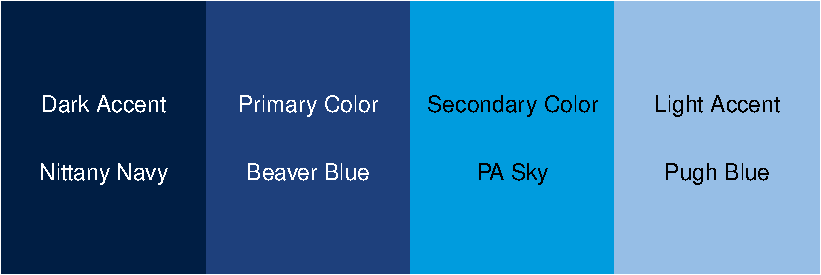
\includegraphics{BOAST_style_guide_files/figure-latex/bluePalette-1} 

}

\caption{The Blue Palette}\label{fig:bluePalette}
\end{figure}

Here is what the Blue Palette looks like in action:

\begin{figure}

{\centering 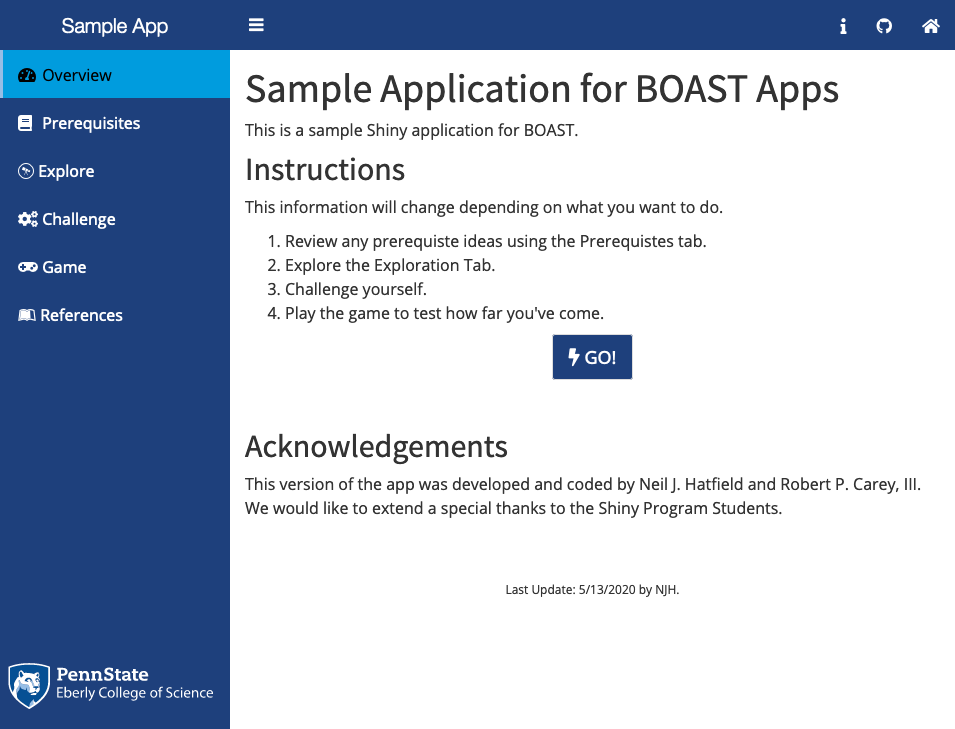
\includegraphics[width=13.26in]{images/blueOverview} 

}

\caption{Overview Page Using the Blue Palette}\label{fig:blueAction1}
\end{figure}

\begin{figure}

{\centering 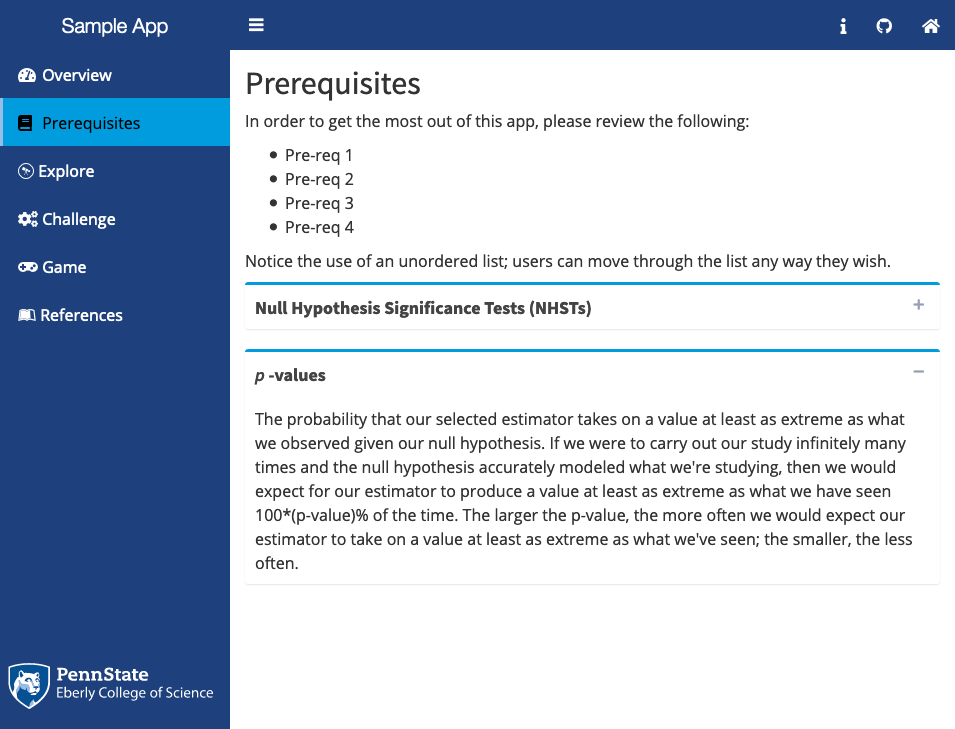
\includegraphics[width=13.26in]{images/blueCollapse} 

}

\caption{Collapsible Boxes Using the Blue Palette}\label{fig:blueAction2}
\end{figure}

\begin{figure}

{\centering 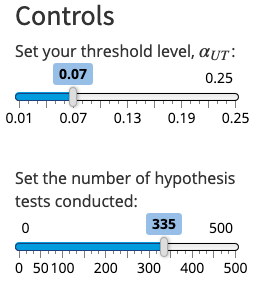
\includegraphics{images/blueSliders} 

}

\caption{Sliders Using the Blue Palette}\label{fig:blueAction3}
\end{figure}

\hypertarget{green}{%
\paragraph{Green}\label{green}}

The Green Palette looks like the following:

\begin{figure}

{\centering 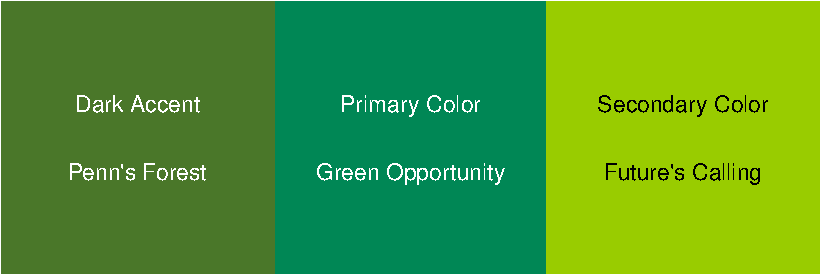
\includegraphics{BOAST_style_guide_files/figure-latex/greenPalette-1} 

}

\caption{The Green Palette}\label{fig:greenPalette}
\end{figure}

Here is what the Green Palette looks like in action:

\begin{figure}

{\centering 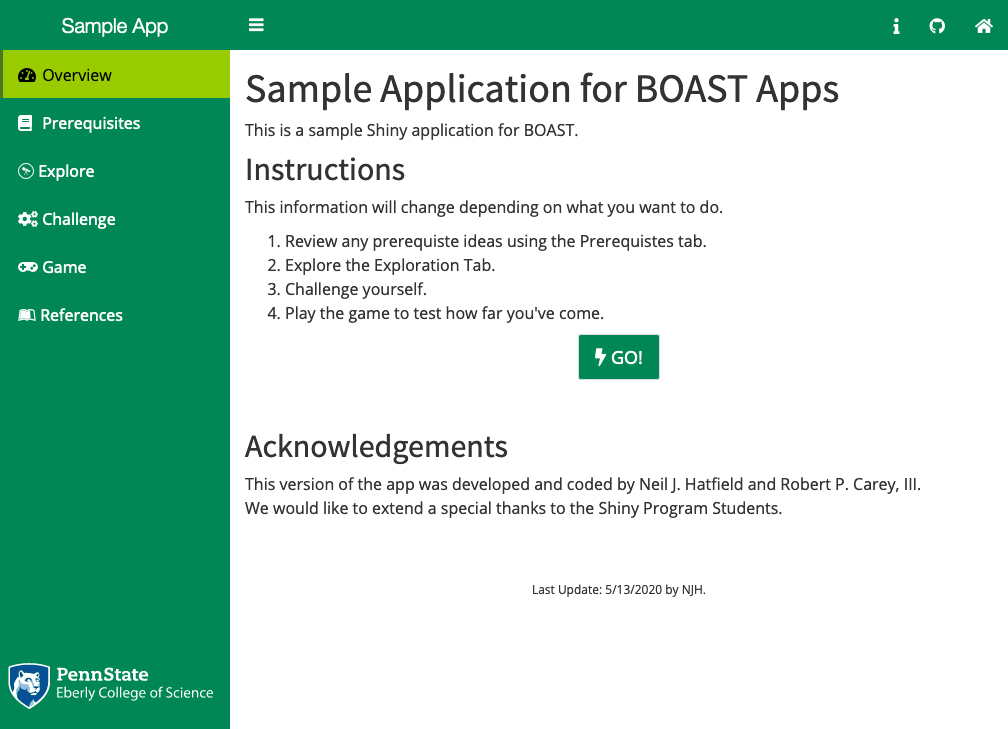
\includegraphics[width=14in]{images/greenOverview} 

}

\caption{Overview Page Using the Green Palette}\label{fig:greenAction1}
\end{figure}

\begin{figure}

{\centering 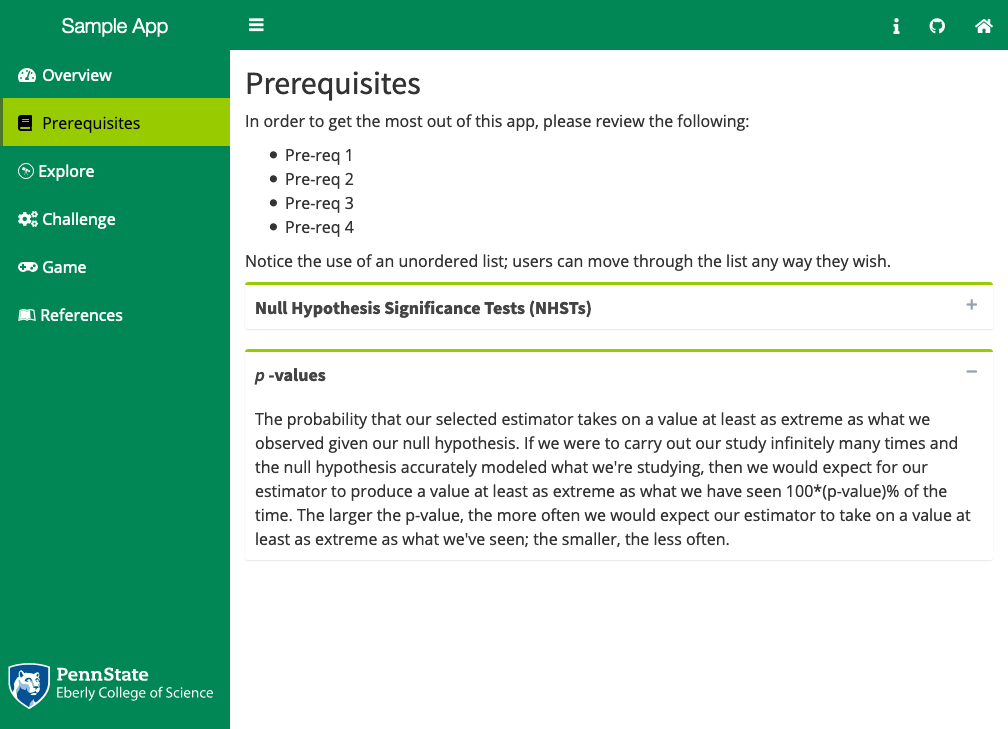
\includegraphics[width=14in]{images/greenCollapse} 

}

\caption{Collapsible Boxes Using the Green Palette}\label{fig:greenAction2}
\end{figure}

\begin{figure}

{\centering 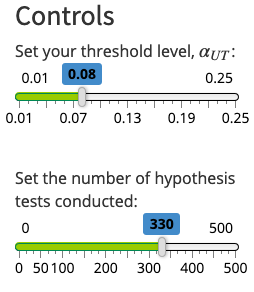
\includegraphics{images/greenSliders} 

}

\caption{Sliders Using the Green Palette}\label{fig:greenAction3}
\end{figure}

\hypertarget{purple}{%
\paragraph{Purple}\label{purple}}

The Purple Palette looks like the following:

\begin{figure}

{\centering 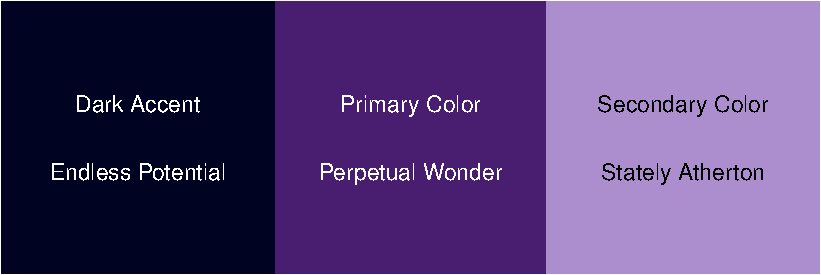
\includegraphics{BOAST_style_guide_files/figure-latex/purplePalette-1} 

}

\caption{The Purple Palette}\label{fig:purplePalette}
\end{figure}

Here is what the Purple Palette looks like in action:

\begin{figure}

{\centering 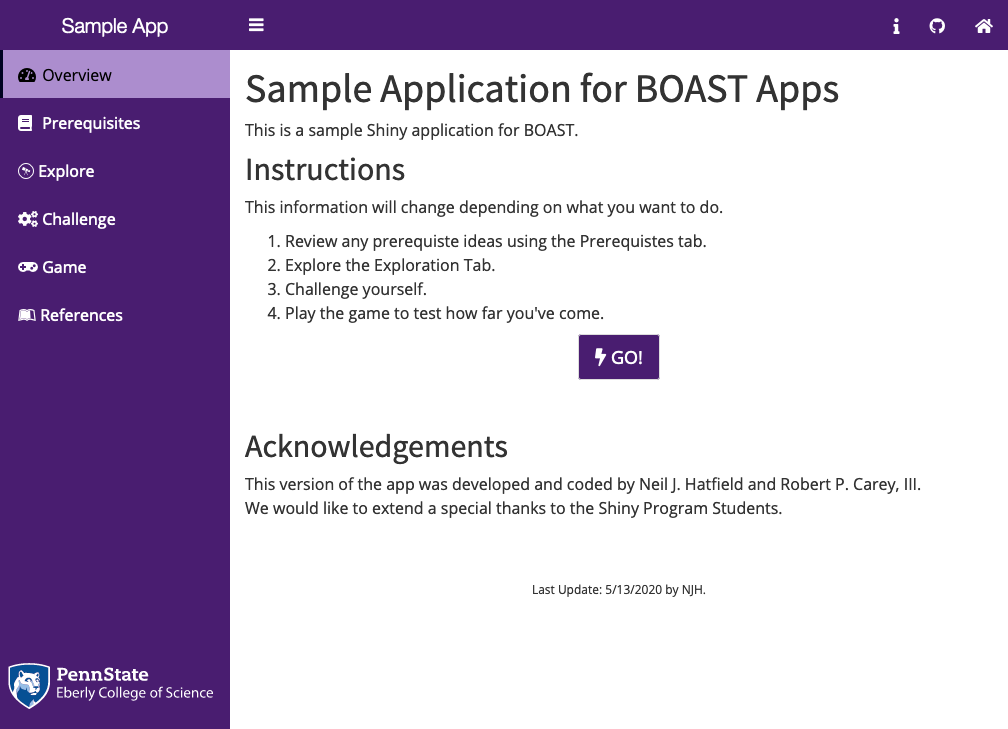
\includegraphics[width=14in]{images/purpleOverview} 

}

\caption{Overview Page Using the Purple Palette}\label{fig:purpleAction1}
\end{figure}

\begin{figure}

{\centering 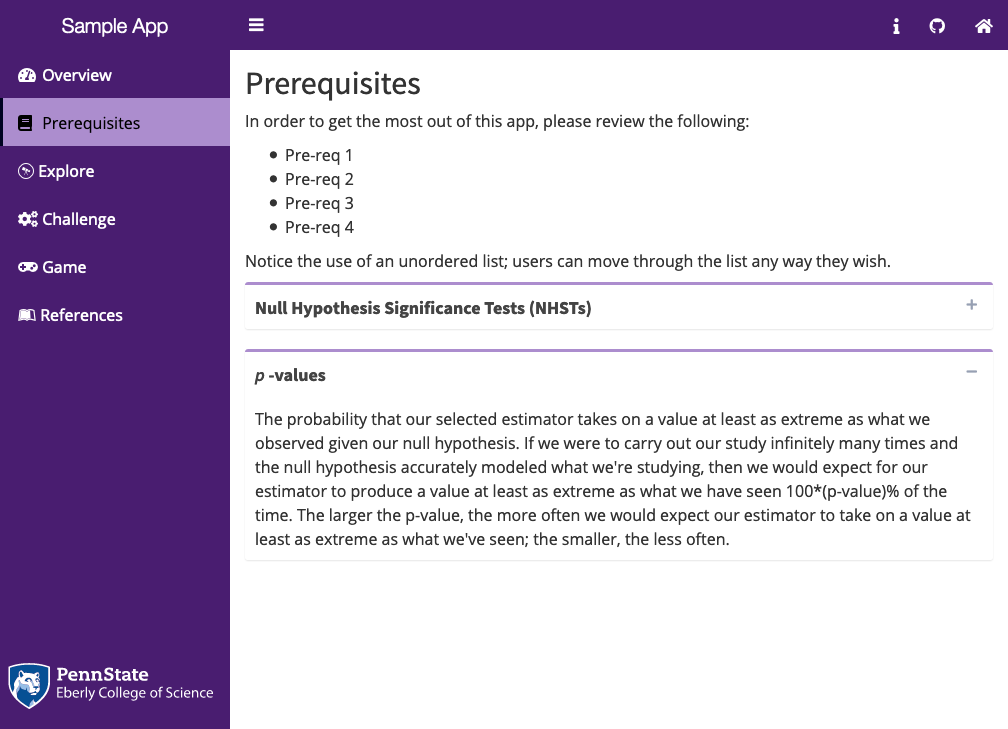
\includegraphics[width=14in]{images/purpleCollapse} 

}

\caption{Collapsible Boxes Using the Purple Palette}\label{fig:purpleAction2}
\end{figure}

\begin{figure}

{\centering 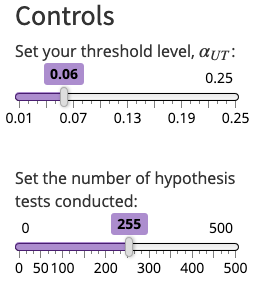
\includegraphics{images/purpleSliders} 

}

\caption{Sliders Using the Purple Palette}\label{fig:purpleAction3}
\end{figure}

\hypertarget{black}{%
\paragraph{Black}\label{black}}

The ``Black'' Palette is not pegged to the color black, but rather teal/aqua colors. However, to call the theme in the Shiny dashboard, the user must use the value \texttt{black} for the the \texttt{skin} argument. Here's what the ``Black'' Palette looks like:

\begin{figure}

{\centering 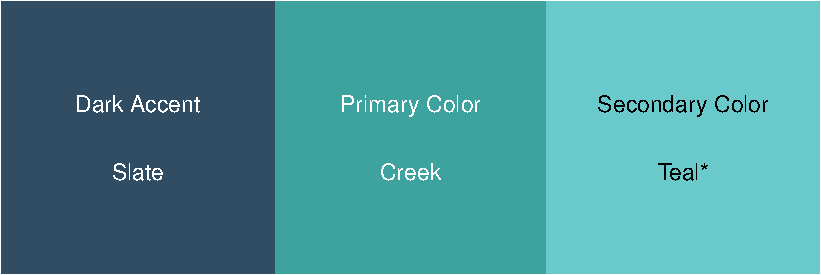
\includegraphics{BOAST_style_guide_files/figure-latex/blackPalette-1} 

}

\caption{The 'Black' Palette}\label{fig:blackPalette}
\end{figure}

Here is what the ``Black'' Palette looks like in action:

\begin{figure}

{\centering 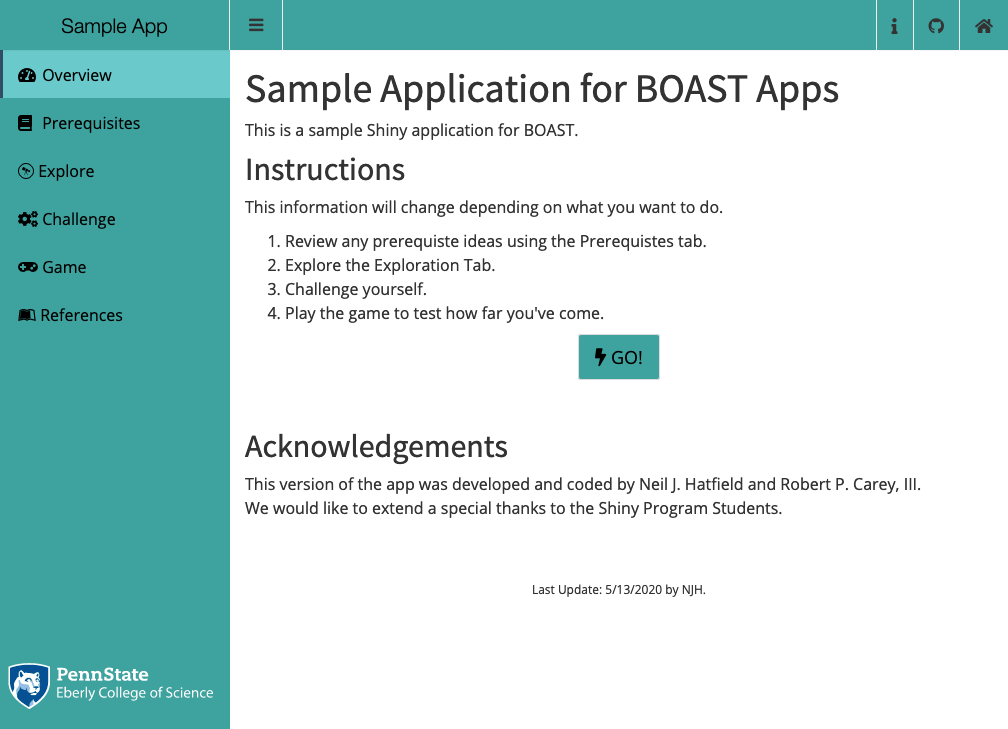
\includegraphics[width=14in]{images/blackOverview} 

}

\caption{Overview Page Using the 'Black' Palette}\label{fig:blackAction1}
\end{figure}

\begin{figure}

{\centering 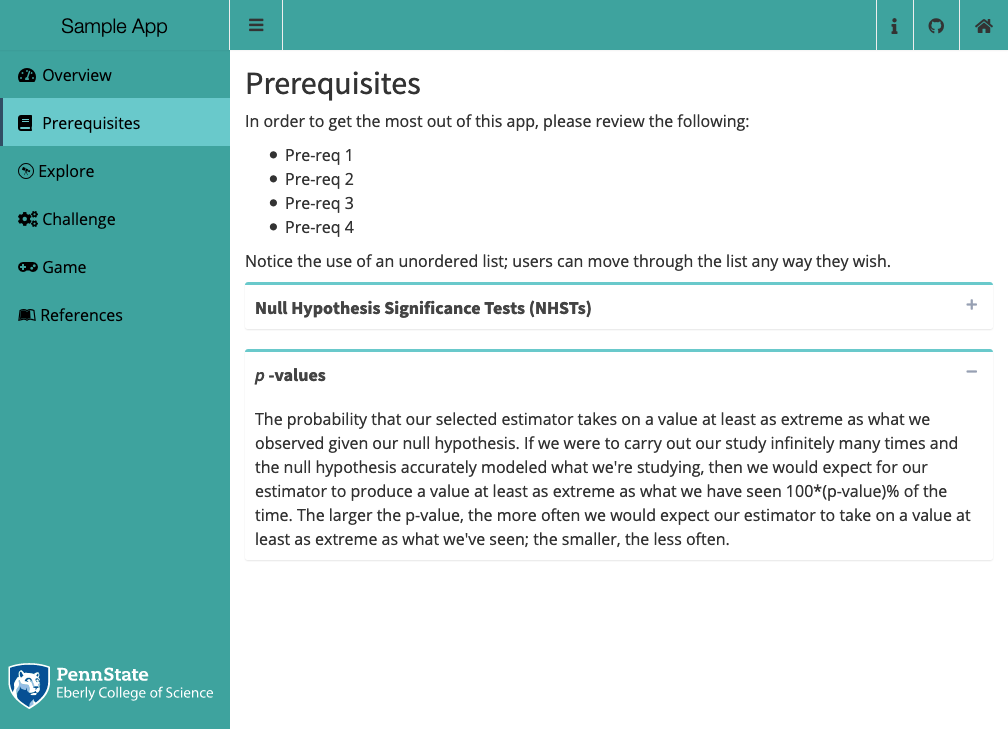
\includegraphics[width=14in]{images/blackCollapse} 

}

\caption{Collapsible Boxes Using the 'Black' Palette}\label{fig:blackAction2}
\end{figure}

\begin{figure}

{\centering 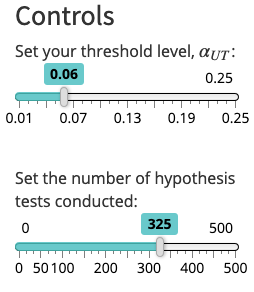
\includegraphics{images/blackSliders} 

}

\caption{Sliders Using the 'Black' Palette}\label{fig:blackAction3}
\end{figure}

\hypertarget{yellow}{%
\paragraph{Yellow}\label{yellow}}

The Yellow Palette is still under consideration. The current set looks like the following:

\begin{figure}

{\centering 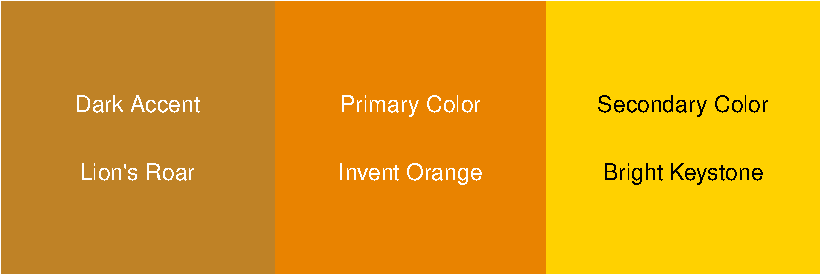
\includegraphics{BOAST_style_guide_files/figure-latex/yellowPalette-1} 

}

\caption{The Yellow Palette}\label{fig:yellowPalette}
\end{figure}

Here is what the Yellow Palette looks like in action:

\begin{figure}

{\centering 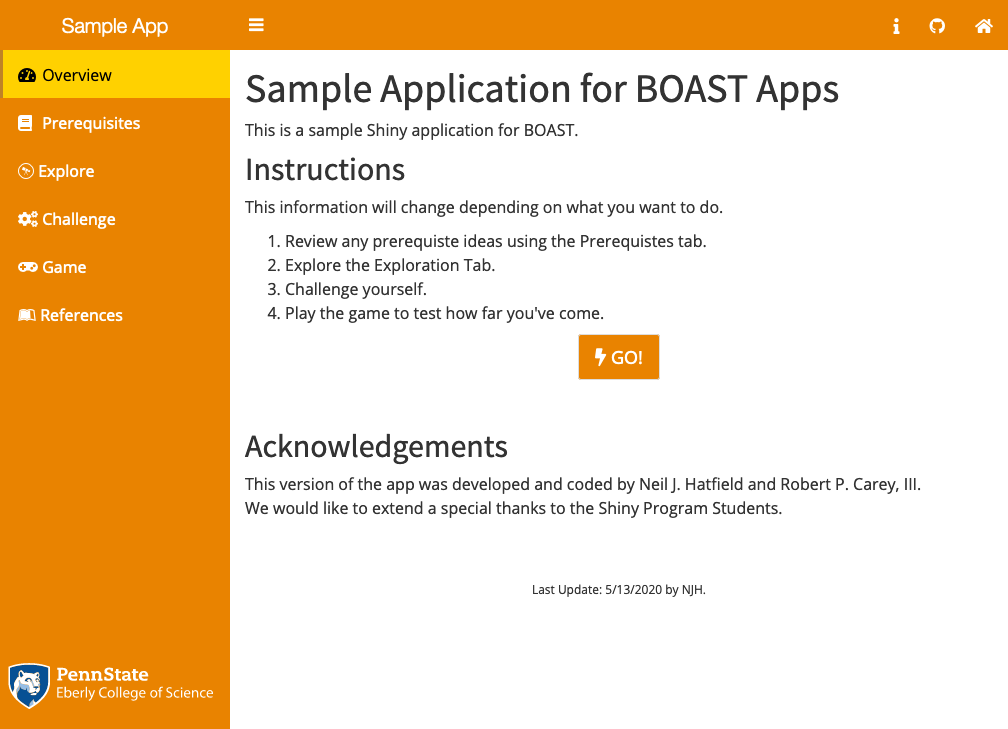
\includegraphics[width=14in]{images/yellowOverview} 

}

\caption{Overview Page Using the Yellow Palette}\label{fig:yellowAction1}
\end{figure}

\begin{figure}

{\centering 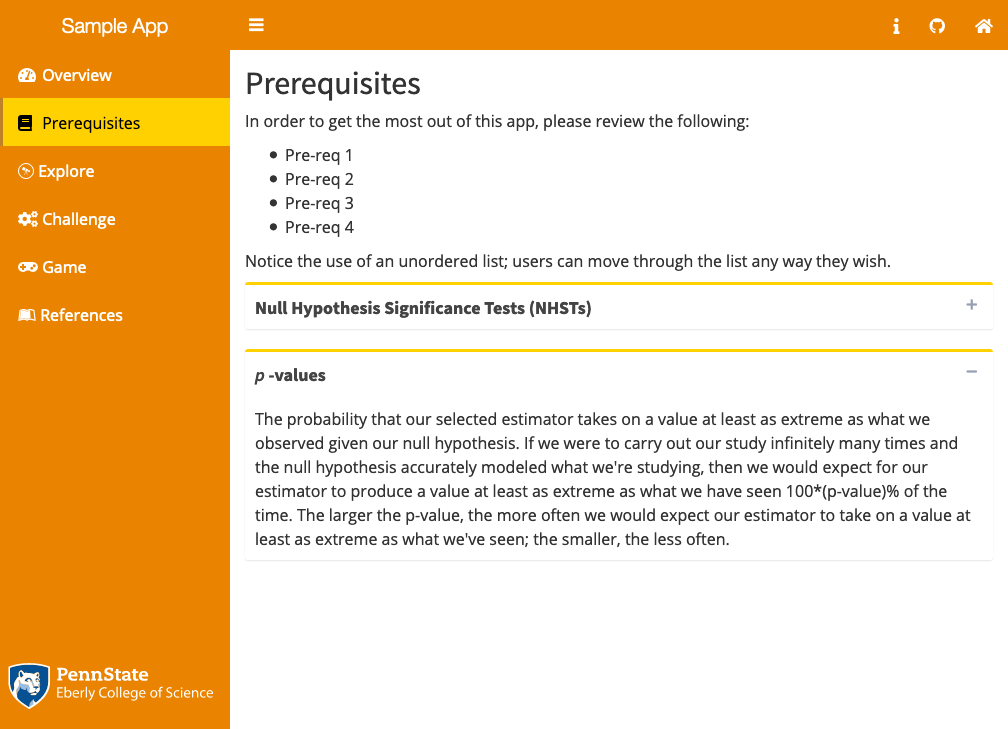
\includegraphics[width=14in]{images/yellowCollapse} 

}

\caption{Collapsible Boxes Using the Yellow Palette}\label{fig:yellowAction2}
\end{figure}

\begin{figure}

{\centering 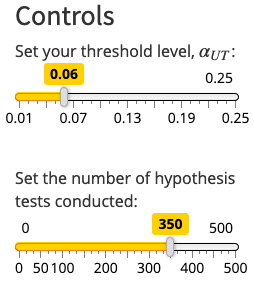
\includegraphics{images/yellowSliders} 

}

\caption{Sliders Using the Yellow Palette}\label{fig:yellowAction3}
\end{figure}

\hypertarget{red}{%
\paragraph{Red}\label{red}}

The Red Palette is still under construction. Here's the current set:

\begin{figure}

{\centering 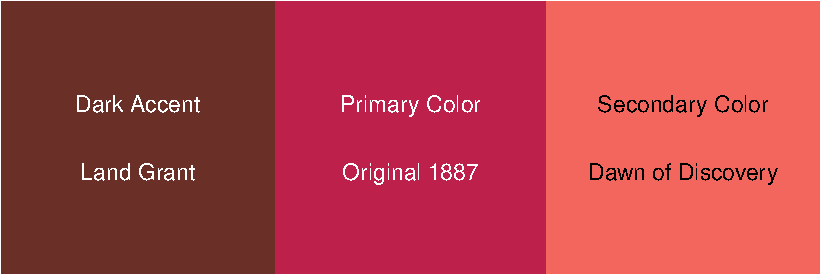
\includegraphics{BOAST_style_guide_files/figure-latex/redPalette-1} 

}

\caption{The Red Palette}\label{fig:redPalette}
\end{figure}

Here is what the Red Palette looks like in action:

\begin{figure}

{\centering 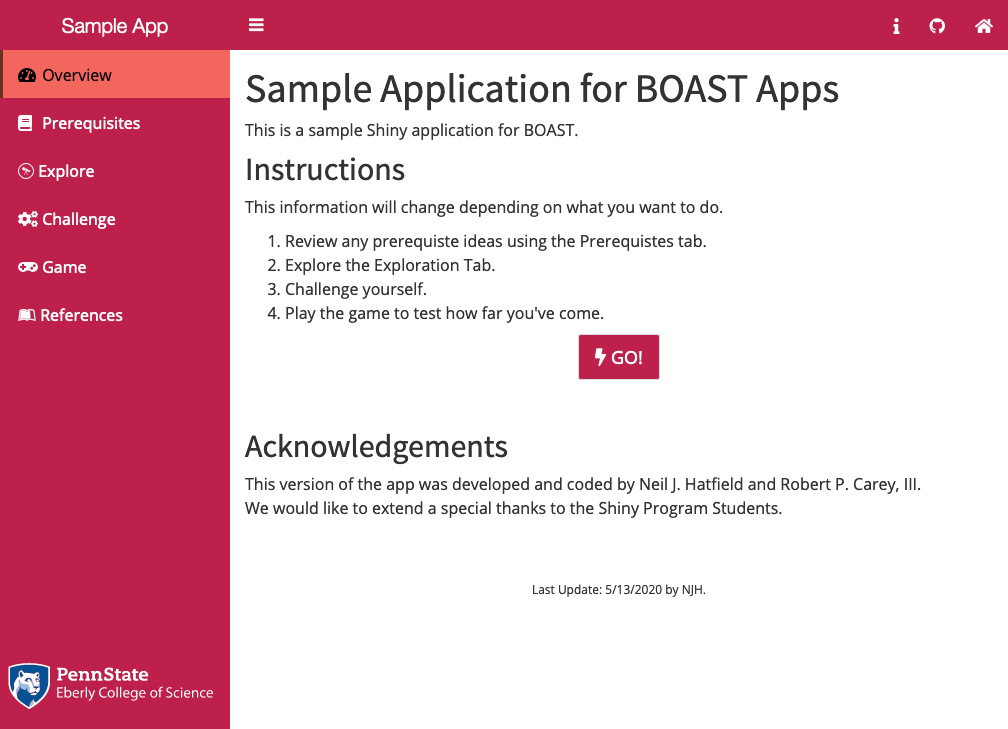
\includegraphics[width=14in]{images/redOverview} 

}

\caption{Overview Page Using the Red Palette}\label{fig:redAction1}
\end{figure}

\begin{figure}

{\centering 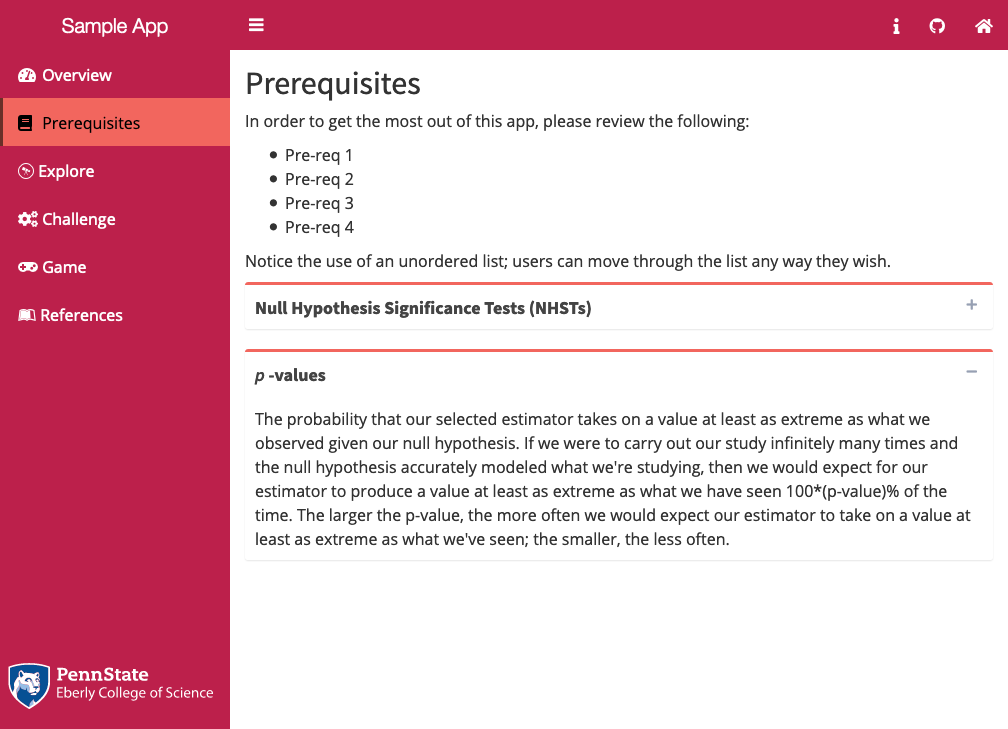
\includegraphics[width=14in]{images/redCollapse} 

}

\caption{Collapsible Boxes Using the Red Palette}\label{fig:redAction2}
\end{figure}

\begin{figure}

{\centering 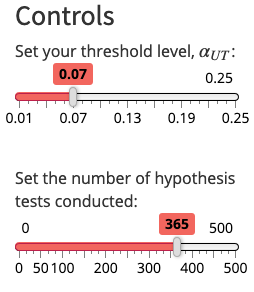
\includegraphics{images/redSliders} 

}

\caption{Sliders Using the Red Palette}\label{fig:redAction3}
\end{figure}

\hypertarget{chapterColor}{%
\subsection{Current Chapter Color Assignments}\label{chapterColor}}

Here are the current (05/27/2020) color theme assignments for chapters:

\begin{itemize}
\tightlist
\item
  Chapter 1: Data Gathering RED
\item
  Chapter 2: Data Description YELLOW
\item
  Chapter 3: Basic Probability BLUE
\item
  Chapter 4: Statistical Inference PURPLE
\item
  Chapter 5: Probability BLUE
\item
  Chapter 6: Regression ``BLACK''
\item
  Chapter 7: ANOVA ``BLACK''
\item
  Chapter 8: Time Series PURPLE
\item
  Chapter 9: Sampling RED
\item
  Chapter 10: Categorical Data YELLOW
\item
  Chapter 11: Data Science GREEN
\item
  Chapter 12: Stochastic Processes BLUE
\item
  Chapter 13: Biology GREEN
\end{itemize}

\hypertarget{dashboard-header}{%
\section{Dashboard Header}\label{dashboard-header}}

Each Dashboard Header contains only a couple of elements. The most important of these will be a {[}shortened{]} Title of your App. This will automatically be followed by the sidebar collapse/expand button. At the far right, you will then include a link to the home page of BOAST using the Home icon.

Additional icons might be included to the left of the Home icon. However, these icons remain the same for all Tabs/pages of your App and are thus are not appropriate for Tab/page specific information.

There should not be any additional elements in the Dashboard Header. Any links for navigate in your App should appear in the Sidebar on the left edge.

The width of the Title component of the Header should be 300; \texttt{titleWidth\ =\ 300}.

\hypertarget{dashboard-sidebar}{%
\section{Dashboard Sidebar}\label{dashboard-sidebar}}

\hypertarget{last-element}{%
\subsection{Last Element}\label{last-element}}

The last element of the Sidebar will be the Penn State Logo. Please refer to the Section \ref{logo}.

\hypertarget{dashboard-body}{%
\section{Dashboard Body}\label{dashboard-body}}

The Sidebar (responsible for App navigation) and the Body are intimately related to one another. The Sidebar provides structure to your App as well as being the primary way that a user can move around the App. The Body is where all content (text, images, plots, buttons, etc.) exists for the user to read, view, and interact with.

The Sidebar should have a width of 300, (\texttt{width\ =\ 300}).

To ensure a consistent experience across all apps, you need to make sure that your App has the following tabs/page, in the following order:

\hypertarget{the-overview-tab}{%
\subsection{The Overview Tab}\label{the-overview-tab}}

This Tab is \textbf{REQUIRED} for all Apps. This is the main landing page of your App and should appear at the top of the sidepanel.

The icon for this Tab must be ``dashboard''.

The Overview Tab must contain \textbf{ALL} of the following elements:

\begin{enumerate}
\def\labelenumi{\arabic{enumi}.}
\tightlist
\item
  ``Title'' (as Heading 1)
\item
  A description of the app (as paragraph text under the title)
\item
  ``Instructions'' (as Heading 2)
\item
  General instructions for using the App (using an Ordered List environment)
\item
  A button that will take the user to the next Tab/page.
\item
  ``Acknowledgements'' (as Heading 2)
\item
  A listing of acknowledgements including, coders, content writers, etc. (as a paragraph)
\item
  Last Element: \texttt{div(class\ =\ "updated",\ "Last\ Update:\ mm/dd/yyyy\ by\ FL.")} with mm/dd/yyyy replaced with the date of the update you pushed to the server and FL replaced with your initials.
\end{enumerate}

There is no need to use boldface or colons with the section headings when you properly use Heading tags. Thus, ``Instructions:'' does not follow this Style Guide. Additionally, there should not be an ``About'' heading.

\hypertarget{a-prerequisites-tab}{%
\subsection{A Prerequisites Tab}\label{a-prerequisites-tab}}

If your App needs to ensure that the user has the base understandings necessary to interact with your App, you'll need to create a prerequisites Tab. Otherwise, skip this Tab.

The icon for this Tab must be ``book''.

Use the word ``Prerequisites'' rather than ``Pre-reqs'', ``Prereqs'', or ``Pre-requisites''.

\hypertarget{types-of-prerequisites}{%
\subsubsection{Types of Prerequisites}\label{types-of-prerequisites}}

There are two different types of prerequisites: technical/conceptual and contextual. Both of these go into the Prerequisites tab.

Technical/Conceptual Prerequisites cover ideas that the user needs in order to fully engage with your App's statistical goal. For instance, if your App is about ANCOVA, the ideas of ANOVA and building a linear model would be good candidates for technical/conceptual prerequisites.

Contextual Prerequisites cover ideas that which are beneficial for the user to understand a context you're using. For example, if you are referencing an astragalus, you should include a brief explanation and/or picture of an astragalus.

Keep in mind that Contextual Prerequisites are different than context which should be part of the Activity Tab. If the information is necessary to interpret sliders/graphs and is \emph{specific}, then you should include this information in the Activity Tab. If the information helps the user say ``Oh, that's what they mean by {[}blank{]}'', that is good sign of something to put in the Prerequisites Tab.

\hypertarget{text-links-in-prerequisites-and-beyond}{%
\subsubsection{Text Links in Prerequisites (and Beyond)}\label{text-links-in-prerequisites-and-beyond}}

In as many instances as possible, we would like to provide the user with a link to Online Notes of a World Campus Statistics course.

\emph{Note: what appears here is applicable any time you want to link to an webpage that is beyond BOAST.}

The link that you provide must take the user to the appropriate location. Do not send the user to the home page for a course; rather, take them to the relevant page. To do this, you'll need to explore the \href{https://online.stat.psu.edu/statprogram/}{Department of Statistics STAT ONLINE} page and look through the courses.

You will create these links in-line, not as a button. Thus, they must be part of a paragraph block (i.e., inside a \texttt{p()} with other text) or as part of list item (i.e., inside a \texttt{li()}).

Your link must include descriptive text. Using ``Click Here'' is \textbf{not} descriptive. Rather say where the link will take the user. If you look through the links that we've included in this Style Guide, we've been modeling this. This descriptive text not only helps all users anticipate where they are going but also improves the accessibility of the links. (Plus, have you ever tried to click a small link on your phone?)

Once you find the appropriate page, you'll need to copy the URL for your link. There are some instances where we might be able to find an existing anchor (look for two inter-locking rings to appear when you place your cursor over a title) or make a request for adding an anchor. These are especially useful if what you want to link to is only part of the page.

*Note: not all requests for anchors may be fulfilled and not all course notes have anchors.

The styling of the link will be managed by the BOAST CSS file.

Here's are two examples of how you would code a text link:

\begin{Shaded}
\begin{Highlighting}[]
\CommentTok{# [omitted code]}
\CommentTok{# Working in the UI section}

\CommentTok{# Example 1: in a paragraph}
\KeywordTok{p}\NormalTok{(}\StringTok{"While not critical, you might wish to refresh your understanding on some of the basic shapes}
\StringTok{  of graphs in statistics. A good resource for this would be the "}\NormalTok{, }\CommentTok{# Notice the ending space}
\NormalTok{  tags}\OperatorTok{$}\KeywordTok{a}\NormalTok{(}
    \DataTypeTok{herf =} \StringTok{"https://online.stat.psu.edu/stat100/lesson/3/3.2#graphshapes"}\NormalTok{, }\CommentTok{#the URL}
    \StringTok{"STAT 100 Table of Graph Shapes"} \CommentTok{# the descriptive text for the link}
\NormalTok{    ),}
  \StringTok{". Feel free to check that resource out."} 
  \CommentTok{# Notice the ending punctuation for the prior sentence is not part of the link.}
\NormalTok{)}

\CommentTok{# Example 2: in a list item}
\NormalTok{tags}\OperatorTok{$}\KeywordTok{ul}\NormalTok{(}
\NormalTok{  tags}\OperatorTok{$}\KeywordTok{li}\NormalTok{(}\StringTok{"Review the "}\NormalTok{, }\CommentTok{# Notice the ending space}
\NormalTok{    tags}\OperatorTok{$}\KeywordTok{a}\NormalTok{(}
      \DataTypeTok{herf =} \StringTok{"https://online.stat.psu.edu/stat100/lesson/3/3.2#graphshapes"}\NormalTok{, }\CommentTok{#the URL}
      \StringTok{"STAT 100 Table of Graph Shapes"} \CommentTok{# the descriptive text for the link}
\NormalTok{      )}
    \CommentTok{# List items don't necessarily need ending punctuation. }
    \CommentTok{#Be consistent; either all items do or none.}
\NormalTok{  ) }
\NormalTok{)}
\CommentTok{# [omitted code]}
\end{Highlighting}
\end{Shaded}

\hypertarget{activity-tabs}{%
\subsection{Activity Tab(s)}\label{activity-tabs}}

This is the heart of your App and you are required to have at least one.

In the event you have multiple activities, each one will need a separate Tab. The order of these Tabs will depend upon the your goals for the App.

Each Tab should contain all information/instructions for the user to be able to interact with the activity without having to switch to other Tabs.

The icon you use depends on the type of activity:

\begin{itemize}
\tightlist
\item
  Games will use the icon ``gamepad''.
\item
  Explorations will use the icon ``wpexplorer''.
\item
  Challenges will use the icon ``gears''.
\end{itemize}

\hypertarget{general-layout-for-activity-tabs}{%
\subsubsection{General Layout for Activity Tabs}\label{general-layout-for-activity-tabs}}

For the vast majority of Activity Tabs, we will adopt a 3-part layout:

\begin{itemize}
\tightlist
\item
  Across the top will be any general information the user needs to interact with your App as well as an context information.
\item
  To the left and wrapped in a well panel will be the inputs/controls that the user will need to manipulate.
\item
  To the right and NOT in a well panel will be the outputs (graphs, images, R output)
\end{itemize}

There will be some cases where this general layout does not necessarily work. For instance, Tic-Tac-Toe games will not follow this layout.

\hypertarget{references}{%
\subsection{References}\label{references}}

The last Tab will be for your references. This Tab is \textbf{REQUIRED} and is where you will place a reference list for all of the following items that you used in your app:

\begin{itemize}
\tightlist
\item
  All \texttt{R} packages you used
\item
  Sources of any Code you used directly or drew heavily upon from other people
\item
  Pictures and/or other images
\item
  Data sets
\item
  Refer to the Documentation Section (\ref{documentation}) of this Style Guide for more information.
\end{itemize}

The icon for this Tab must be ``leanpub''.

\hypertarget{tabs-inside-the-body}{%
\subsection{Tabs Inside the Body}\label{tabs-inside-the-body}}

There are two types of tabs in a Shiny app: there are the \texttt{tabItem} (i.e., the pages within an app and should appear in the Sidebar) and \texttt{tabPanel} (i.e., creating sub-pages or independent sections). In this section, we will discuss this later case.

Deciding on whether to use \texttt{tabPanel} is going to depend on several things:

\begin{enumerate}
\def\labelenumi{\arabic{enumi}.}
\tightlist
\item
  Do you have two or more aspects that are related enough that they shouldn't be their own separate tabs/pages of your App?

  \begin{enumerate}
  \def\labelenumii{\alph{enumii}.}
  \tightlist
  \item
    If NO, then you shouldn't use \texttt{tabPanel}.\\
  \item
    If YES, then continue.
  \end{enumerate}
\item
  Are any of your aspects something that would be better suited as a Challenge or Game tab?

  \begin{enumerate}
  \def\labelenumii{\alph{enumii}.}
  \tightlist
  \item
    If YES, move that aspect to a separate page. If you still have 2+ aspects, continue.\\
  \item
    If NO, continue.\\
  \end{enumerate}
\item
  Are the aspects independent enough that a person can skip a couple and still use the App successfully?

  \begin{enumerate}
  \def\labelenumii{\alph{enumii}.}
  \tightlist
  \item
    If NO, then you should re-consider your design.\\
  \item
    If YES, then proceed with using \texttt{tabPanel} in you design.
  \end{enumerate}
\end{enumerate}

When you go to make a set of tab panels you will need to first create a \texttt{tabsetPanel} which will wrap around all of the individual panels. Use \texttt{type\ =\ "tabs"}.

The tabs inside the body should automatically appear horizontally and along the top of the tab body (i.e., in the white space below the Dashboard Header). Any visual styling will be managed by the BOAST CSS file at a global level.

\hypertarget{common-elements}{%
\section{Common Elements}\label{common-elements}}

In addition to the Dashboard elements of the apps, there are other elements that are common. This include things such as how inputs should be ordered, buttons, correct/incorrect indicators, and animation buttons.

For information about popovers, rollovers, hover text, or tooltips, please see Section \ref{popovers}.

\hypertarget{ordering-inputs}{%
\subsection{Ordering Inputs}\label{ordering-inputs}}

One of the most powerful aspects of Shiny apps is that the user interacts with them. Thus, we do need to consider not only the ways in which user interact (e.g., buttons, sliders, text entry, etc.) but also the order in which you want the user to manipulate the inputs. Coming up with a single declaration for how to order inputs in all cases is not necessarily feasible. However, we can set up a general guideline for how to make decisions on ordering your inputs.

Please use the following guidelines for determining the order of inputs in the User Interface (UI):

\begin{enumerate}
\def\labelenumi{\arabic{enumi}.}
\tightlist
\item
  In general, if you want your user to do things in certain order, make your inputs appear in that order. For example, If you want them to pick a data set, then an unusualness threshold/significance level, what attribute to test, and then set a parameter value, then your inputs should appear in that order.
\item
  Make use of how we read the English language, i.e., Top-to-Bottom and Left-to-Right to provide an implicit ordering for your user.
\item
  If a user needs to carry out steps in particular sequence for your App to run properly, then place your inputs inside of an Ordered List environment with explicit text on what they should do. For example,

  \begin{enumerate}
  \def\labelenumii{\arabic{enumii}.}
  \tightlist
  \item
    Choose your data set: {[}dropdown{]}\\
  \item
    Set your unusualness threshold/significance level\\
    {[}slider{]}\\
  \item
    Which attribute do you want to test: {[}dropdown{]}\\
  \item
    What parameter value do you want to use: {[}numeric input{]}
  \end{enumerate}
\item
  If an input is going to reset other inputs you should either:

  \begin{enumerate}
  \def\labelenumii{\alph{enumii}.}
  \tightlist
  \item
    Warn the user before hand\\
  \item
    Move the input to the top of the list\\
  \item
    Program the input to not reset other inputs\\
  \item
    Some combination of the above\\
  \end{enumerate}
\item
  If the inputs are not dynamically linked to the output (e.g., plots automatically update with a change in the input's value), then you should include a button that says ``Make Plot'' at the end of the inputs.
\end{enumerate}

\hypertarget{buttons}{%
\subsection{Buttons}\label{buttons}}

Buttons are one way in which users interact with the apps. The two most common functions that are used are \texttt{shiny::actionButton} and \texttt{shinyBS::bsButton}. Both functions share many of the same features. Two ways in which they are different is that \texttt{shinyBS::bsButton} has an additional \texttt{style} argument while \texttt{shiny::actionButton} has a \texttt{width} argument that gives you fine grain size control (\texttt{bsButton} just has a qualitative size option). There are three key styling aspects: shape/animation, color, and text \& icon.

\hypertarget{shapeanimation}{%
\subsubsection{Shape/Animation}\label{shapeanimation}}

All shape aspects of buttons will be controlled by CSS. The standard shape will be rectangular (the default). Sizing will be controlled by CSS although setting \texttt{size\ =\ "large"} for the \texttt{bsButton} call may be done.

We have a number of apps where a button will change shape/size when a person hovers their cursor over it. This ``animation'' is to be discontinued. This is to say that buttons which change shape/size should be flagged as issues and resolved at the first opportunity.

At most, the button's color might change (e.g., lighten or darken), depending on the context.

\hypertarget{color}{%
\subsubsection{Color}\label{color}}

The coloring of the button will also be controlled by CSS in one of two ways.

The default way will be through the BOAST CSS. This will ensure that the selected color scheme for your App will be consistent.

The second way only applies to \texttt{bsButton} and the \texttt{style} argument. Here, this option references an external CSS file beyond BOAST. We see these most often in games. Use the following list to guide you in choosing which style:

\begin{itemize}
\tightlist
\item
  \texttt{warning}: Good for when you want the user to proceed with caution; for example a submit button in a game.
\item
  \texttt{danger}: Good for when you want the user to think twice before clicking; for example, a reset game button.
\item
  \texttt{success}: Good for when you want to convey that the user can proceed safely; for example, a button that advances the user through the game
\item
  \texttt{info}: Good for when you want to give some additional information; for example, a button that triggers game instructions popping up, a button that gives a hint, or a button that might filter a question pool.
\end{itemize}

When in doubt, use the the \texttt{default} style option (or even omit this argument) for \texttt{bsButton} or use \texttt{actionButton}.

\hypertarget{text-icon}{%
\subsubsection{Text \& Icon}\label{text-icon}}

The last styling element of a button is two-fold: the text that is in the button and the icon.

Here are some guidelines for text of a button:

\begin{itemize}
\tightlist
\item
  All buttons must have some text.
\item
  Generally speaking, the text should be relatively brief and clear.

  \begin{itemize}
  \tightlist
  \item
    Don't use ``Go to the next page'' when you could use ``Next''
  \end{itemize}
\item
  The text should make sense with the action of the button; for example,

  \begin{itemize}
  \tightlist
  \item
    ``Reset'' if the button resets something (a game, a plot, inputs)
  \item
    ``Submit'' if the button triggers the app to grab and process input values
  \item
    ``Make Graph'' if button causes a graph to be generated
  \item
    ``Show/Hide Graph'' if a button makes a graph object appear/disappear
  \item
    ``Next'' if a button moves the user along some path.
  \end{itemize}
\item
  If the button references something like a particular tab (prerequisites, exploration, etc.), the text should reflect this.

  \begin{itemize}
  \tightlist
  \item
    ``Explore!'' for a button that takes a user to an Exploration tab.
  \item
    ``Prerequisites'' for a button that takes a user to a Prerequisites tab.
  \item
    ``Challenge Yourself!'' for a button takes a user to a Challenge tab.
  \item
    ``Play!'' for a button that takes a user to Game tab.
  \end{itemize}
\item
  If a button references an object like an activity packet or a download prompt the text should refer to that

  \begin{itemize}
  \tightlist
  \item
    ``Activity Packet'' for a button that would open up and/or download a packet for the user
  \item
    ``Download Data'' for a button that would download a data file.
  \end{itemize}
\item
  Clarity is essential. If there are multiple buttons on the page, make sure that you use clear text for what button does and/or references.
\end{itemize}

Here are guidelines for the inclusion of icons in a button:

\begin{itemize}
\tightlist
\item
  Game buttons will NOT have any icons.
\item
  Direction Buttons (e.g., ``Next'' or ``Previous'') will NOT have any icons. Rather make the button text ``\textless\textless{} Previous'' or ``Next \textgreater\textgreater{}''
\item
  A ``Prerequisites'' button will use the ``book'' icon
\item
  All other tab buttons (labels ending with ``!'') will use the ``bolt'' icon.
\item
  A download button will use the ``cloud-download'' icon.
\end{itemize}

\hypertarget{correctincorrect-marks}{%
\subsection{Correct/Incorrect Marks}\label{correctincorrect-marks}}

In games, you can give the user a visual cue as to whether they are correct or incorrect through the use of two images:

\begin{figure}

{\centering 
\includegraphics[width=3.75in]{images/check} 
\includegraphics[width=3.75in]{images/cross} 

}

\caption{Correct/Incorrect Marks}\label{fig:marks}
\end{figure}

You can save these two images by right-clicking on them and selecting ``Save Image As\ldots{}''. You will need to put them in the \texttt{www} folder/directory of your App.

Their placement in your App will depend upon what makes the most sense.

\hypertarget{animation-buttons}{%
\subsection{Animation Buttons}\label{animation-buttons}}

One feature of slider inputs is the option to include a Play/Pause button that allows the user to create an animation of your plot. Enabling this option can be quite useful if allowing the user to move through the whole set of slider values is desirable.

To enable this, you'll need to make use of the \texttt{animate} argument:

\begin{Shaded}
\begin{Highlighting}[]
\CommentTok{#[code omitted]}
\KeywordTok{sliderInput}\NormalTok{(}
  \DataTypeTok{inputId =} \StringTok{"mtcAlpha"}\NormalTok{,}
  \DataTypeTok{label =} \StringTok{"Set your threshold level, }\CharTok{\textbackslash{}\textbackslash{}}\StringTok{(}\CharTok{\textbackslash{}\textbackslash{}}\StringTok{alpha_\{UT\}}\CharTok{\textbackslash{}\textbackslash{}}\StringTok{):"}\NormalTok{,}
  \DataTypeTok{min =} \FloatTok{0.01}\NormalTok{,}
  \DataTypeTok{max =} \FloatTok{0.25}\NormalTok{,}
  \DataTypeTok{value =} \FloatTok{0.1}\NormalTok{,}
  \DataTypeTok{step =} \FloatTok{0.01}\NormalTok{,}
  \DataTypeTok{animate =} \KeywordTok{animationOptions}\NormalTok{(}
    \DataTypeTok{interval =} \DecValTok{1000}\NormalTok{, }\DataTypeTok{loop =} \OtherTok{TRUE}\NormalTok{))}

\CommentTok{#[code omitted]}
\end{Highlighting}
\end{Shaded}

You can set \texttt{animate=TRUE}, \texttt{animate=FALSE} or invoke the \texttt{animationOptions} function as we've done in the example and recommend. This will force you to make some important decisions: namely, how long the slider should wait between each movement (\texttt{interval}, in milliseconds) and should the animation start over once the slider reaches the maximum (\texttt{loop}).

The \texttt{interval} is going to the most challenging value to figure out. This timer \emph{\textbf{ignores}} everything else; that is, it doesn't wait to see whether your plot has updated. Remember, the more complicated the process is that generates your plot, the longer your App will need to render the plot. Thus, you can quickly get into a case where the slider has advanced several times while your App is still trying to render the first update. While \texttt{renderCachePlot} can help speed things up, keep in mind that you still might need to play around with the \texttt{interval} value to ensure smooth functionality.

Make sure when you're testing an animated slider to vary all of the parameters involved in the graph. This will help ensure that you test adequately.

The styling of the play/pause button will be controlled by the BOAST CSS file.

\hypertarget{progress-bar}{%
\subsection{Progress Bar}\label{progress-bar}}

Consider adding a loading bar to show the process for intense computations; this will help the user understand that your App is processing and not frozen/broken.

\hypertarget{designStyle}{%
\chapter{Design Style}\label{designStyle}}

This chapter of the BOAST Style Guide deals with the Visual Appearance of each app. Visual Styling encompasses not only text styling but also color scheme usage, graphics (images, plots, tables), and the dashboard layout. For each app, there are 6 major components to the Visual Appearance that you will need to consider: PSU Branding, the Dashboard, Common Elements, Color, Text Styling, and Graphics.

One of the most important benefits of using the \texttt{boastApp} function from the \texttt{boastUtils} package is that is that much of the Visual Appearance will be automatically handled for you. However, you should still familiarize yourself with the Visual Appearance Style for our apps.

\hypertarget{logo}{%
\section{PSU Branding}\label{logo}}

Given that we are all associated with Pennsylvania State University, we need to include the Penn State logo in each App. Rather than sticking the logo at the top of the Overview page, we are going to place the logo at the bottom of the sidebar. This has the benefit of having the logo appear throughout the entire App AND making the logo be as unobtrusive as possible.

In your UI section of \texttt{app.R} (or the \texttt{ui.R} file), at the end of the \texttt{dashboardSidebar()} section, you will need to include the following:

\begin{Shaded}
\begin{Highlighting}[]
\NormalTok{tags}\OperatorTok{$}\KeywordTok{div}\NormalTok{(}\DataTypeTok{class =} \StringTok{"sidebar-logo"}\NormalTok{,}
\NormalTok{         boastUtils}\OperatorTok{::}\KeywordTok{psu_eberly_logo}\NormalTok{(}\StringTok{"reversed"}\NormalTok{))}
\end{Highlighting}
\end{Shaded}

Here's how this code would look in context:

\begin{Shaded}
\begin{Highlighting}[]
\KeywordTok{dashboardPage}\NormalTok{(}
  \DataTypeTok{skin =} \StringTok{"blue"}\NormalTok{,}
  \KeywordTok{dashboardHeader}\NormalTok{(}
    \DataTypeTok{title =} \StringTok{"title"}\NormalTok{,}
    \CommentTok{# [omitted code]}
\NormalTok{  ),}
  \KeywordTok{dashboardSidebar}\NormalTok{(}
    \DataTypeTok{width =} \DecValTok{300}\NormalTok{,}
    \KeywordTok{sidebarMenu}\NormalTok{(}
      \DataTypeTok{id =} \StringTok{"tabs"}\NormalTok{,}
      \CommentTok{# [omitted code],}
\NormalTok{      tags}\OperatorTok{$}\KeywordTok{div}\NormalTok{(}
        \DataTypeTok{class =} \StringTok{"sidebar-logo"}\NormalTok{,}
\NormalTok{        boastUtils}\OperatorTok{::}\KeywordTok{psu_eberly_logo}\NormalTok{(}\StringTok{"reversed"}\NormalTok{)}
\NormalTok{        )}
\NormalTok{      ),}
    \KeywordTok{dashboardBody}\NormalTok{(}
\NormalTok{    tags}\OperatorTok{$}\KeywordTok{head}\NormalTok{(}
\NormalTok{      tags}\OperatorTok{$}\KeywordTok{link}\NormalTok{(}\DataTypeTok{rel =} \StringTok{"stylesheet"}\NormalTok{, }\DataTypeTok{type =} \StringTok{"text/css"}\NormalTok{,}
        \DataTypeTok{href =} \StringTok{"https://educationshinyappteam.github.io/Style_Guide/theme/boast.css"}\NormalTok{),}
      \KeywordTok{tabItems}\NormalTok{(}
       \CommentTok{# [omitted code]}
\NormalTok{      )  )  )  )  )}
\end{Highlighting}
\end{Shaded}

This will ensure that the Penn State logo gets properly used.

\hypertarget{colors}{%
\section{Colors}\label{colors}}

Your App needs to have a consistent color scheme throughout. The color scheme should be checked against colorblindness to meet \href{https://www.w3.org/WAI/WCAG21/quickref/}{WCAG 2.1} Level AA. You can do so at the \href{https://davidmathlogic.com/colorblind/\#\%23000000-\%23E69F00-\%2356B4E9-\%23009E73-\%23F0E442-\%230072B2-\%23D55E00-\%23CC79A7}{Coloring for Colorblindness} website. If you are following this Style Guide (as you should be) then the vast majority of this section will be automatically handled for you.

There are two major places where coloring comes into play: the user interface and plots you generate in \texttt{R}.

\hypertarget{styleText}{%
\section{Text Styling}\label{styleText}}

Text styling refers the non-content aspects of the text on the page. This means things such as the use of italics, boldface, alignment, as well as font size and color.

You should let the centralized CSS file do the heavy lifting for text styling. (Again, using \texttt{boastApp} will help you.) However, for this to work properly, you will need to tag content appropriately. (See the HTML section: \ref{html})

If you run into a situation where some element needs additionl styling, \textbf{talk to Neil or Bob for help}. You might have come across an element that needs to get added the central CSS file or a bug.

\hypertarget{headings}{%
\subsection{Headings}\label{headings}}

Use the Heading Tags for the short fragments that define the structure of your App. If you find yourself enclosing a complete sentence in Heading tag, you ARE NOT using headings correctly. Notice how the headings in this Style Guide aren't complete sentences; your App should mimic this. Full sentences appear as regular paragraph text (i.e., enclosed in \texttt{p()}) and not be a Heading.

\hypertarget{paragraph-text}{%
\subsection{Paragraph Text}\label{paragraph-text}}

If you enclose text that gives instructions or other information to your App's users in \texttt{p()} or \texttt{li()} (the later should be wrapped in either \texttt{tags\$ol()} or \texttt{tags\$ul()}), your App will understand how to style that text correctly. The central CSS file contains controls that set the base font size much larger than Shiny does natively as well as making text sizing dynamic. (This is important for making our apps mobile device friendly.) Again, using \texttt{boastApp} makes this process easier.

If you want to make a certain word or phrase italic, you will need to wrap that text in \texttt{tags\$em()}. Similarly, if you want do the same with boldface, you'll use \texttt{tags\$strong()}.

For example, this code:

\begin{Shaded}
\begin{Highlighting}[]
\KeywordTok{p}\NormalTok{(}
  \StringTok{"When dealing with the "}\NormalTok{,}
\NormalTok{  tags}\OperatorTok{$}\KeywordTok{em}\NormalTok{(}\StringTok{"t"}\NormalTok{),}
  \StringTok{"-distribution, we only have one parameter, the "}\NormalTok{,}
\NormalTok{  tags}\OperatorTok{$}\KeywordTok{strong}\NormalTok{(}\StringTok{"degrees of freedom"}\NormalTok{),}
  \StringTok{"that we need to input."}
\NormalTok{)}
\end{Highlighting}
\end{Shaded}

Becomes:

\begin{quote}
When dealing with the \emph{t}-distribution, we only have one parameter, the \textbf{degrees of freedom} that we need to input.
\end{quote}

Use italics (emphasis), and boldface (strong) sparingly.

\hypertarget{mathematics}{%
\subsection{Mathematics}\label{mathematics}}

For the most part, any mathematics you need displayed should be done using \href{https://www.mathjax.org/}{MathJax}. Default to using inline typesetting with the \texttt{\textbackslash{}\textbackslash{}(} and \texttt{\textbackslash{}\textbackslash{})} delimiters. If you need to use display style, you can use \texttt{\textbackslash{}\textbackslash{}{[}} and \texttt{\textbackslash{}\textbackslash{}{]}}. For the vast majority of mathematics, you'll wrap both inline and display style mathematics inside of a paragraph environment (\texttt{p()}).

If you're writing mathematics directly in your app, remember you'll need to escape the LaTeX commands by putting an extra backslash (\textbackslash) in front; e.g., \texttt{\textbackslash{}frac\{3\}\{4\}} would need to be \texttt{\textbackslash{}\textbackslash{}frac\{3\}\{4\}}.

If you're reading in mathematical text from an external CSV file, you do not need the extra backslash in the CSV file.

If you need assistance in figuring out how to type up mathematics, please talk to Neil, Matt, or Dennis.

\textbf{Note:} Double dollar sign delimiters are generally not recommended for displaying math as they can lead to unintended results. See: \href{https://docs.mathjax.org/en/latest/basic/mathematics.html}{Writing Mathematics for MathJax}.

\hypertarget{game-question-text}{%
\subsection{{[}Game{]} Question Text}\label{game-question-text}}

The text used as a question in a game should NOT be wrapped in a Heading tag; wrap the text in a paragraph tag.

\hypertarget{label-text-buttons-sliders-other-inputs-and-alerts}{%
\subsection{Label Text (Buttons, Sliders, Other Inputs and Alerts)}\label{label-text-buttons-sliders-other-inputs-and-alerts}}

By using the central CSS file, any text you included in/on buttons, dropdown menus, sliders, radio buttons, choices, and other inputs as well as alert messages and popups/rollovers, will automatically be styled correctly.

Do not use heading tags, the paragraph tag, italics/emphasis, or boldface/strong with input labels. Input labels should be written in sentence case (i.e., capitalize only the first word and any proper nouns).

You may use these tags with popups/rollovers.

\hypertarget{feedback-and-hint-text}{%
\subsection{Feedback and Hint Text}\label{feedback-and-hint-text}}

Again, let the central CSS file handle the styling of this type of text.

\hypertarget{text-in-r-plots}{%
\subsection{\texorpdfstring{Text in \texttt{R} Plots}{Text in R Plots}}\label{text-in-r-plots}}

Unfortunately, any text in \texttt{R} plots does not get controlled by CSS. This means that you'll have to play around with the settings. Using the \texttt{ggplot2} package to make your plots (or other packages based upon the ggplot framework) will allow you to use the \texttt{theme} aspect to control text in your App.

Here is an example for how to do this:

\begin{Shaded}
\begin{Highlighting}[]
\CommentTok{# Create a ggplot2 object}
\NormalTok{g1 <-}\StringTok{ }\NormalTok{ggplot2}\OperatorTok{::}\KeywordTok{ggplot}\NormalTok{(}\DataTypeTok{data=}\NormalTok{df, }\KeywordTok{aes}\NormalTok{(}\DataTypeTok{x=}\NormalTok{x, }\DataTypeTok{y=}\NormalTok{y, }\DataTypeTok{color=}\NormalTok{grp)) }
\CommentTok{# Add your layers, for example}
\NormalTok{g1 }\OperatorTok{+}\StringTok{ }\NormalTok{ggplot2}\OperatorTok{::}\KeywordTok{geom_point}\NormalTok{()}
\CommentTok{# Use theme to control text size}
\NormalTok{g1 }\OperatorTok{+}\StringTok{ }\NormalTok{ggplot2}\OperatorTok{::}\KeywordTok{theme}\NormalTok{(}
  \DataTypeTok{plot.caption =} \KeywordTok{element_text}\NormalTok{(}\DataTypeTok{size =} \DecValTok{18}\NormalTok{),}
  \DataTypeTok{text =} \KeywordTok{element_text}\NormalTok{(}\DataTypeTok{size =} \DecValTok{18}\NormalTok{)}
\NormalTok{  )}
\end{Highlighting}
\end{Shaded}

You will need to play around with the settings to find the appropriate value; text size 18 appears to work out well in many cases.

\textbf{Note:} The text in your plot might not behave well for dynamic resizing on different mobile devices.

\hypertarget{graphics}{%
\section{Graphics}\label{graphics}}

One of the most powerful tools we have in Statistics and Data Science is graphics. This includes images/pictures, graphs/plots, and tables. You will want to make sure that all graphical elements are appropriately sized in the Body. If there is text in a static image/picture, you'll need to make sure that the text is legible on a variety of screen sizes.

We've already discussed both issues of color and text size in plots. For additional considerations, please refer to the following readings (ordered from most important to least):

\begin{itemize}
\tightlist
\item
  \href{https://www.dropbox.com/s/hb52991v09p8q91/Tufte\%20-\%202006\%20-\%20The\%20Fundamental\%20principles\%20of\%20analytical\%20design.pdf?dl=0}{Tufte-Fundamental Principles of Analytical Design}
\item
  \href{https://www.dropbox.com/s/z8yrf4eqph6c2h4/Tufte\%20-\%202001\%20-\%20Chartjunk\%20Vibrations\%2C\%20grids\%2C\%20and\%20ducks.pdf?dl=0}{Tufte-Chartjunk}\\
\item
  \href{https://www.dropbox.com/s/62uegsribwdjtze/Kosslyn\%20-\%202006\%20-\%20Looking\%20with\%20the\%20eye\%20and\%20mind.pdf?dl=0}{Kosslyn-Looking with the Eye and Mind}
\end{itemize}

Remember, we always want to be modeling excellent graphing behaviors.

\begin{quote}
All photographs can be fortified with words. --Dorothea Lange
\end{quote}

\begin{quote}
A picture is worth a thousand words\ldots but which ones. --Unknown
\end{quote}

Both of these quotations highlight that you need to include some text with your plots to help the user construct their understanding of what you're trying to show them.

\hypertarget{titles-and-labels}{%
\subsection{Titles and Labels}\label{titles-and-labels}}

Graph and Table titles should follow Title Case. Capitalize each word unless the word is ``small'' (e.g., of, an, etc.). The \href{https://titlecase.com/}{Title Case website} can help you if you aren't sure. (This website also does other types of case such as camel case.)

\hypertarget{axes-and-scales}{%
\subsection{Axes and Scales}\label{axes-and-scales}}

\texttt{R}'s default axes are terrible. They often do not fully cover the data and the have gaps between the axes. All this impedes the user's construction of meaning. Thus, you'll want to take control and stipulate the axes and scales to optimize what users get out of the plot. If you are providing multiple plots that the user is supposed to compare, make sure that they all use the same scaling and axes.

To force \texttt{ggplot2} to place (0, 0) in the lower-left corner and to control the scales, you will need to include the following:

\begin{Shaded}
\begin{Highlighting}[]
\CommentTok{# Create the ggplot2 object}
\NormalTok{g1 <-}\StringTok{ }\NormalTok{ggplot2}\OperatorTok{::}\KeywordTok{ggplot}\NormalTok{(...)}
\CommentTok{# Add your layer}
\NormalTok{g1 }\OperatorTok{+}\StringTok{ }\NormalTok{ggplot2}\OperatorTok{::}\KeywordTok{geom_point}\NormalTok{()}
\CommentTok{# Control axes and scale}
\CommentTok{## Multiplicative Scaling of the Horizontal (x) Axis}
\CommentTok{## Additive Scaling of the Vertical (y) Axis}
\NormalTok{g1 }\OperatorTok{+}\StringTok{ }\NormalTok{ggplot2}\OperatorTok{::}\KeywordTok{scale_x_continuous}\NormalTok{(}\DataTypeTok{expand =} \KeywordTok{expansion}\NormalTok{(}\DataTypeTok{mult =} \KeywordTok{c}\NormalTok{(}\DecValTok{1}\NormalTok{,}\DecValTok{2}\NormalTok{), }\DataTypeTok{add =} \DecValTok{0}\NormalTok{)) }\OperatorTok{+}\StringTok{ }
\StringTok{  }\KeywordTok{scale_y_continuous}\NormalTok{(}\DataTypeTok{expand =} \KeywordTok{expansion}\NormalTok{(}\DataTypeTok{mult =} \DecValTok{0}\NormalTok{, }\DataTypeTok{add =} \KeywordTok{c}\NormalTok{(}\DecValTok{0}\NormalTok{,}\FloatTok{0.05}\NormalTok{))) }
\end{Highlighting}
\end{Shaded}

\hypertarget{color-and-plots-in-r}{%
\subsection{\texorpdfstring{Color and Plots in \texttt{R}}{Color and Plots in R}}\label{color-and-plots-in-r}}

In \texttt{R} you can set color theme which you use in \texttt{ggplot2}. Here are two custom color palettes that you can use in your App. Additionally, the package \texttt{viridis} provides several additional color palettes which are improvements upon the default color scheme.

\begin{Shaded}
\begin{Highlighting}[]
\CommentTok{# boastPalette is based on the Wong color blind set found at the above website.}
\NormalTok{boastPalette <-}\StringTok{ }\KeywordTok{c}\NormalTok{(}\StringTok{"#0072B2"}\NormalTok{,}\StringTok{"#D55E00"}\NormalTok{,}\StringTok{"#009E73"}\NormalTok{,}\StringTok{"#CE77A8"}\NormalTok{,}
    \StringTok{"#000000"}\NormalTok{,}\StringTok{"#E69F00"}\NormalTok{,}\StringTok{"#999999"}\NormalTok{,}\StringTok{"#56B4E9"}\NormalTok{,}\StringTok{"#CC79A7"}\NormalTok{)}

\CommentTok{# psuPalette is based on Penn State's three official color palettes}
\CommentTok{# and checked at the above webite.}
\NormalTok{psuPalette <-}\StringTok{ }\KeywordTok{c}\NormalTok{(}\StringTok{"#1E407C"}\NormalTok{,}\StringTok{"#BC204B"}\NormalTok{,}\StringTok{"#3EA39E"}\NormalTok{,}\StringTok{"#E98300"}\NormalTok{,}
    \StringTok{"#999999"}\NormalTok{,}\StringTok{"#AC8DCE"}\NormalTok{,}\StringTok{"#F2665E"}\NormalTok{,}\StringTok{"#99CC00"}\NormalTok{)}

\CommentTok{# Both palettes get used in the order of what is listed.}
\end{Highlighting}
\end{Shaded}

To use these palettes (or ones from \texttt{viridis}) with a \texttt{ggplot2} object, you'll need to doe the following

\begin{Shaded}
\begin{Highlighting}[]
\CommentTok{# You will need to first add whichever palette line from above to your code}
\NormalTok{boastPalette <-}\StringTok{ }\KeywordTok{c}\NormalTok{(}\StringTok{"#0072B2"}\NormalTok{,}\StringTok{"#D55E00"}\NormalTok{,}\StringTok{"#009E73"}\NormalTok{,}\StringTok{"#CE77A8"}\NormalTok{,}
    \StringTok{"#000000"}\NormalTok{,}\StringTok{"#E69F00"}\NormalTok{,}\StringTok{"#999999"}\NormalTok{,}\StringTok{"#56B4E9"}\NormalTok{,}\StringTok{"#CC79A7"}\NormalTok{)}

\CommentTok{# Create ggplot2 object}
\NormalTok{g1 <-}\StringTok{ }\NormalTok{ggplot2}\OperatorTok{::}\KeywordTok{ggplot}\NormalTok{(}\DataTypeTok{data =}\NormalTok{ df, }
                \KeywordTok{aes}\NormalTok{(}\DataTypeTok{x =}\NormalTok{ x, }\DataTypeTok{y =}\NormalTok{ y, }\DataTypeTok{color =}\NormalTok{ grp, }\DataTypeTok{fill =}\NormalTok{ grp))}
\CommentTok{# Add your layers}
\NormalTok{g1 }\OperatorTok{+}\StringTok{ }\NormalTok{ggplot2}\OperatorTok{::}\KeywordTok{geom_points}\NormalTok{()}
\CommentTok{# Tell R to use your chosen palette}
\NormalTok{g1 }\OperatorTok{+}\StringTok{ }\NormalTok{ggplot2}\OperatorTok{::}\KeywordTok{scale_color_manual}\NormalTok{(}\DataTypeTok{values=}\NormalTok{boastPalette)  }\CommentTok{# If you use "color" in aes}
\NormalTok{g1 }\OperatorTok{+}\StringTok{ }\NormalTok{ggplot2}\OperatorTok{::}\KeywordTok{scale_fill_manual}\NormalTok{(}\DataTypeTok{values=}\NormalTok{boastPalette)  }\CommentTok{# If you use "fill" in aes}
\end{Highlighting}
\end{Shaded}

If you have more groups than eight/nine colors listed in the two palettes, consider reworking your examples as you could overwhelm the user with too many colors. (This also applies to using different shapes to plot points.)

With any eye towards accessibility, try not to use only color to denote a particular piece of information. Rather you might want to use color and shape.

\hypertarget{tables}{%
\subsection{Tables}\label{tables}}

Data tables can pose a challenge for individuals to comprehend. Just as a wall of text isn't conducive to helping a person understand what's going on, neither is a wall of data values. Thus, we need to be extreme judicious about incorporating data tables into any of our apps.

In web development there are two main types of tables: layout tables and data tables.

\begin{itemize}
\tightlist
\item
  Layout tables help to control where different elements appear on the page.
\item
  We need an additional distinction for data tables:

  \begin{itemize}
  \tightlist
  \item
    Summary Data Tables are tables that have summary information; typified by two-way tables (a.k.a. contingency tables or crosstabs) but might also include other things such as values of descriptive statistics stratified by groups.
  \item
    Data Set are an entire data object, presented in tabular format
  \end{itemize}
\end{itemize}

\textbf{Layout Tables should never be used in a BOAST App.}

Data Sets should be displayed \textbf{as sparingly as possible}. In order to include a Data Set display, you will need to have identified an explicit learning goal/objective that necessitates the user digging through a data frame. If you can't identify such a learning goal, you should NOT include a data frame.

If the goal is to allow the user to look through the data set OR to have access to the data, then \textbf{give a link} to either the original source of the data (\textbf{preferred}) or for them to download the file.

Summary Data Tables can be used more often and can enrich the user's experience with your app. However, these must still be constructed in an appropriate manner.

Neither Data Sets nor Summary Data Tables should be inserted into your App as a picture. This is an big Accessibility violation. Use the directions below to create the appropriate type of data table.

\hypertarget{displaying-data-tables}{%
\subsubsection{Displaying Data Tables}\label{displaying-data-tables}}

Your first step is to create a data frame object in your \texttt{R} code.

\begin{itemize}
\tightlist
\item
  If you are displaying a data set (rare), then you will either need to read in the data or call that data frame. For this example, I'll be using the \texttt{mtcars} data frame that is part of \texttt{R}.
\item
  If you are making a Summary Data Table, you'll need to either use \texttt{R} to calculate the values and store in a data frame or create a data frame yourself.
\end{itemize}

In either case, be sure you identify what columns you're going to use. If your original data file has 50 columns, but your App only makes use of 5, drop the the other 45. Only display the columns that you actually use.

Your next step is to decide on where to put this display (e.g., inside an Exploration Tab or as a separate page). This will help you identify where in your App's UI section you need to put the appropriate code.

To ensure that your data table is accessible and responsive (i.e., mobile friendly), you will need to use the \texttt{DT} package.

\begin{Shaded}
\begin{Highlighting}[]
\KeywordTok{install.packages}\NormalTok{(}\StringTok{"DT"}\NormalTok{)}
\CommentTok{# Be sure to include this in your library call}
\KeywordTok{library}\NormalTok{(DT)}
\end{Highlighting}
\end{Shaded}

In your UI section, you'll need to use the following code, placed in the appropriate area:

\begin{Shaded}
\begin{Highlighting}[]
\CommentTok{# [code omitted]}
\NormalTok{DT}\OperatorTok{::}\KeywordTok{DTOutput}\NormalTok{(}\DataTypeTok{outputId =} \StringTok{"mtCars"}\NormalTok{)}
\CommentTok{# [code omitted]}
\end{Highlighting}
\end{Shaded}

Then, in your Server section, you'll need to use the following code:

\begin{Shaded}
\begin{Highlighting}[]
\CommentTok{# [code omitted]}
\CommentTok{# Prepare your data set with only the columns needed}
\NormalTok{carData <-}\StringTok{ }\NormalTok{mtcars[,}\KeywordTok{c}\NormalTok{(}\StringTok{"mpg"}\NormalTok{, }\StringTok{"cyl"}\NormalTok{, }\StringTok{"hp"}\NormalTok{, }\StringTok{"gear"}\NormalTok{, }\StringTok{"wt"}\NormalTok{)]}

\CommentTok{## Use Short but Meaningful Column Names}
\KeywordTok{names}\NormalTok{(carData) <-}\StringTok{ }\KeywordTok{c}\NormalTok{(}\StringTok{"MPG"}\NormalTok{, }\StringTok{"# of Cylinders"}\NormalTok{, }\StringTok{"Horsepower"}\NormalTok{, }\StringTok{"# of Gears"}\NormalTok{, }\StringTok{"Weight"}\NormalTok{)}

\CommentTok{# Create the output data table}
\CommentTok{# Be sure to use the same name as you did in the UI}
\NormalTok{output}\OperatorTok{$}\NormalTok{mtCars <-}\StringTok{ }\NormalTok{DT}\OperatorTok{::}\KeywordTok{renderDT}\NormalTok{(}
  \DataTypeTok{expr =}\NormalTok{ carData,}
  \DataTypeTok{caption =} \StringTok{"Motor Trend US Data, 1973-1974 Models"}\NormalTok{, }\CommentTok{# Add a caption to your table}
  \DataTypeTok{style =} \StringTok{"bootstrap4"}\NormalTok{, }\CommentTok{# You must use this style}
  \DataTypeTok{rownames =} \OtherTok{TRUE}\NormalTok{,}
  \DataTypeTok{options =} \KeywordTok{list}\NormalTok{( }\CommentTok{# You must use these options}
    \DataTypeTok{responsive =} \OtherTok{TRUE}\NormalTok{, }\CommentTok{# allows the data table to be mobile friendly}
    \DataTypeTok{scrollX =} \OtherTok{TRUE}\NormalTok{, }\CommentTok{# allows the user to scroll through a wide table}
    \DataTypeTok{columnDefs =} \KeywordTok{list}\NormalTok{(  }\CommentTok{# These will set alignment of data values}
      \CommentTok{# Notice the use of ncol on your data frame; leave the 1 as is.}
      \KeywordTok{list}\NormalTok{(}\DataTypeTok{className =} \StringTok{'dt-center'}\NormalTok{, }\DataTypeTok{targets =} \DecValTok{1}\OperatorTok{:}\KeywordTok{ncol}\NormalTok{(carData))}
\NormalTok{    )}
\NormalTok{  )}
\NormalTok{)}
\CommentTok{# [code omitted]}
\end{Highlighting}
\end{Shaded}

If you are making a Summary Data Table, you will need to follow the same process. If your data frame does not have row names, but instead a column with values acting as row names, you may replace the \texttt{rownames\ =\ TRUE} with \texttt{rownames\ =\ FALSE}; there should not be a column of sequential numbers on the left.

Column names \textbf{MUST} be simple and \emph{meaningful} to the user. To this end, you should rename any columns that might have poor choices for names, just as we have done with the \texttt{mtcars} data. This includes using Greek characters in isolation. You should not have any columns labeled \(\mu\) or \(\sigma\). Rather you need to use English words.

\emph{Note: getting mathematical expressions to render properly in graphical environments in \texttt{R} is not as easy as in the paragraphs or headers of an app. Only certain graphing packages support limited mathematical expressions. The same is true for table generation packages.}

Again, try to use tables as infrequently as possible. Poorly constructed tables can create accessibility issues causing screen readers to poorly communicate tables to your users. If you run into problems and/or have questions, \textbf{talk to Neil and Bob}.

\hypertarget{static-images}{%
\subsection{Static Images}\label{static-images}}

Static image refers to any image you're using in your App which is not produced by \texttt{R}. These are usually PNG or JPG/JPEG files which you end up calling in the UI portion of your code.

Within your App's folder/directory, there needs to be a sub-folder/directory called \texttt{www}. This is the place where you'll need to place ALL static image files.

\hypertarget{adding-an-image}{%
\subsubsection{Adding an Image}\label{adding-an-image}}

To include the image in your App, you'll need to make use of the image tag, \texttt{img}. When you run your App, Shiny automatically knows to check the \texttt{www} folder any time the \texttt{img} tag gets called. Here is an example supposing that the check mark image for correct answers is in the app's \texttt{www} folder:

\begin{Shaded}
\begin{Highlighting}[]
\CommentTok{#[code omitted]}
\KeywordTok{div}\NormalTok{(}\DataTypeTok{align =} \StringTok{"right"}\NormalTok{,}
    \KeywordTok{img}\NormalTok{(}\DataTypeTok{src =} \StringTok{"check.PNG"}\NormalTok{,}
        \DataTypeTok{alt =} \StringTok{"Success, you are correct"}\NormalTok{,}
        \DataTypeTok{width =} \DecValTok{25}\NormalTok{, }\CommentTok{#these are in pixels}
        \DataTypeTok{height =} \DecValTok{25}\NormalTok{,}
\NormalTok{        ))}
\CommentTok{#[code omitted]}
\end{Highlighting}
\end{Shaded}

You'll notice that we've wrapped the \texttt{img} call in a \texttt{div} call. The \texttt{div} call allows us to specify that we want the image to be right aligned; you could also do left or center. You can replace the \texttt{div} call with the paragraph environment and include text on either side, effectively making your image part of the text.

\begin{Shaded}
\begin{Highlighting}[]
\CommentTok{#[code omitted]}
\KeywordTok{p}\NormalTok{(}\StringTok{"Check your answer here -->"}\NormalTok{,}
  \KeywordTok{img}\NormalTok{(}\DataTypeTok{src =} \StringTok{"check.PNG"}\NormalTok{,}
      \DataTypeTok{alt =} \StringTok{"Success, you are correct"}\NormalTok{,}
      \DataTypeTok{width =} \DecValTok{25}\NormalTok{, }\DataTypeTok{height =} \DecValTok{25}\NormalTok{),}
  \StringTok{"<-- Check your answer here"}\NormalTok{),}
\CommentTok{#[code omitted]}
\end{Highlighting}
\end{Shaded}

\hypertarget{sizing-and-positioning-your-image}{%
\subsubsection{Sizing and Positioning Your Image}\label{sizing-and-positioning-your-image}}

All image files have a native size that is part of that file. For instance, the check mark image is 270 x 250 pixels. However, we overrode that that sizing with the \texttt{width} and \texttt{height} arguments. How did we decide on 25 x 25? Honestly, through guess and checking. You'll need to think about how you're using the image and let that guide your decision making. There is no one size fits all solution. While finding an optimal size and position for your image can take some time, seeing bad settings is pretty obvious. Feel free to reach out to Neil and Bob for assistance.

\hypertarget{alt-text}{%
\subsection{Alt Text}\label{alt-text}}

Any graphical element you include in your App \textbf{MUST} have an alternative (assistive) text description (``alt text''). This provides a short description of what is in the image or plot for users who are visual impaired. (Tables, when properly formatted will handle this automatically.)

Here are several resources worth checking out:

\begin{itemize}
\tightlist
\item
  \href{https://webaim.org/techniques/alttext/\#basics}{WebAIM Alternative Text Guide}
\item
  \href{https://accessibility.psu.edu/images/alttext/}{Penn State's Image ALT Text Page}
\item
  \href{https://www.w3.org/WAI/tutorials/images/decision-tree/}{W3C's ALT Text Decision Tree}
\end{itemize}

\hypertarget{adding-alt-text-to-static-images}{%
\subsubsection{Adding Alt Text to Static Images}\label{adding-alt-text-to-static-images}}

In the prior section on static images, you saw exactly how to set the alt text; here is a generic example:

\begin{Shaded}
\begin{Highlighting}[]
\CommentTok{#[code omitted]}
\KeywordTok{img}\NormalTok{(}\DataTypeTok{src =} \StringTok{"yourImage.PNG"}\NormalTok{,}
    \DataTypeTok{alt =} \StringTok{"Short description of what's in the pic"}\NormalTok{,}
    \DataTypeTok{width =} \DecValTok{25}\NormalTok{, }\DataTypeTok{height =} \DecValTok{25}\NormalTok{)}
\CommentTok{#[code omitted]}
\end{Highlighting}
\end{Shaded}

\hypertarget{adding-alt-text-graphs}{%
\subsubsection{Adding Alt Text Graphs}\label{adding-alt-text-graphs}}

\emph{This section is under construction.}

\hypertarget{part-linguistics}{%
\part{Linguistics}\label{part-linguistics}}

\hypertarget{wording}{%
\chapter{Wording}\label{wording}}

This chapter focuses on the wording that we use within the BOAST Apps.

\hypertarget{general-guidelines}{%
\section{General Guidelines}\label{general-guidelines}}

When writing the content for your App, you will want to keep in mind that our apps have students as the primary audience. Thus, we need to make sure that we use language that is appropriate. Seek to use complete sentences that convey what you intend. Have someone else take a look at your content and then tell you what they believe the text to be saying. If what they say is consistent with what you intended, great. If not, then you need to revise your text.

\textbf{DO NOT sacrifice clarity and precision/accuracy for
conciseness/brevity.} While we don't necessarily want a wall of text, there should still be some text to assist the user.

Since these apps are for \emph{teaching and learning}, we need to use language that is accurate and supports students in constructing productive meanings. This means that we need to avoid sloppy language, re-enforcing problematic conceptions, and supporting fallacies. For example,

\begin{itemize}
\tightlist
\item
  Sloppy Language: Vagueness

  \begin{itemize}
  \tightlist
  \item
    BAD: ``We want to explore how these averages differ.''
  \item
    NEUTRAL/FAIR: ``We want to explore how these means differ.''
    \_ GOOD: ``We want to explore how the values of the \emph{sample arithmetic mean} (\emph{SAM}) varies between these groups.''
  \end{itemize}
\item
  Sloppy Language: Discussing values of statistics

  \begin{itemize}
  \tightlist
  \item
    BAD: ``The mean is 6.''
  \item
    GOOD: ``The value of the \emph{sample arithematic mean} for this data is 6 units/object.''
  \end{itemize}
\item
  Problematic conceptions

  \begin{itemize}
  \tightlist
  \item
    BAD: ``Probability is the likelihood of an event in relation to all possible events.''
  \item
    GOOD: ``Probability is the long-run relative frequency for us seeing a particular data event given our assumptions. Likelihood is the long-run relative frequency of a set of assumptions being true given our collected data.''
  \end{itemize}
\item
  Fallacies

  \begin{itemize}
  \tightlist
  \item
    BAD: ``We're 95\% confident that the true population proportion is between 0.35 and 0.45.''
  \item
    GOOD: ``If we were to repeat the entire study infinitely many times, then 95\% of the time we will make an interval that captures the true population proportion.''
  \end{itemize}
\end{itemize}

\hypertarget{popovers}{%
\section{Popovers}\label{popovers}}

The term ``Popovers'' refers to any number of different tools on websites that go by other names such as tooltips, rollovers, and hover text. In essence, this tool appears when the user places their cursor over (i.e., hover) or shifts the focus to a trigger object (typically user inputs or graphs). The text then pops up on the screen for the user to view. The function to create one of these in a Shiny app is \texttt{shinyBS::bsPopover}. While these can be powerful, they are often misused, leading to problems. For example, they can prevent the user from actually interacting with portions of your app when they appear.

Popovers are meant to provide short, simple clarifications; quick annotations which enrich the content that is already present. This type of text is meant to be temporary, only appearing for as long as the user is hovering/focusing on the trigger object. Thus, if you are putting information that is critical for a person to successfully use your App in a popover, you are using popovers \textbf{INCORRECTLY}.

Here are few additional sources for reading about Popovers/Tooltips:

\begin{itemize}
\tightlist
\item
  \href{https://uxplanet.org/tooltips-in-ui-design-f63e117aa3d1}{Tooltips in UI Design}
\item
  \href{https://www.appcues.com/blog/tooltips}{Tooltips: How to use this small but mighty UI pattern correctly}
\end{itemize}

Restrict any usage of a popover to something short and non-vital for your App's user. If you do choose to use a popover, you will need to format the popover correctly. Be sure that your function call includes values for the following arguments:

\begin{itemize}
\tightlist
\item
  \texttt{id}: this needs to be the name of the object which will act as the trigger
\item
  \texttt{title}: this will be a string that appears across the top of your popover; use verbs with an understood ``you'' (e.g., ``Investigate!'', ``Remember'', etc.)
\item
  \texttt{content}: this will be the string that you want displayed; shorter is better.
\item
  \texttt{placement}: this will control where the popover appears. Choose the option (top, bottom, left, right) that works best for your space. Ensure that the placement does not cover any controls or other vital information.
\end{itemize}

The visual appearance of the popover will be control by the central BOAST CSS file.

\hypertarget{dealing-with-differing-vocabularies}{%
\section{Dealing with Differing Vocabularies}\label{dealing-with-differing-vocabularies}}

One of the most challenging aspects of Wording is the fact that we have to deal with the Jingle/Jangle problem.

\hypertarget{jingleJangle}{%
\subsection{The Jingle/Jangle Problem}\label{jingleJangle}}

A term ``jingles'' when people use that term to refer to two (or more) different concepts. This is also know as a term having lexical ambiguity. For instance, \emph{random} jingles when people use the term to convey haphazardness, arbitrariness, and/or an attribute of process. (Note: the only the third option is statistically valid.)

On the other hand, a set of 2+ different terms ``jangle'' when they refer to the same concept. A good/classical example of this is skewness. Some people talk about left/right skewness, others negative/positive skewness, and others will talk about long left/long right tails. Each of these pairs refer to the same core concept, but evoke different mental images.

\hypertarget{option-0-dictionarythesaurus}{%
\subsection{Option 0: Dictionary/Thesaurus}\label{option-0-dictionarythesaurus}}

There are a variety of ways in which we could handle this approach. One thought is to build a Dictionary/Thesaurus for BOAST. While we could go down this route, this represents a considerable undertaking and might become a long term goal.

\hypertarget{hovertext}{%
\subsection{Option 1: Hover Text}\label{hovertext}}

The more immediate solution to differing vocabularies is for us to make use of hover text. This approach is appealing in that the user doesn't have to leave your App (like going to a dictionary/thesaurus) and the content of these tips is not critical to using your App. That is to say, the information is available for those who might need a quick reminder but does not take up permanent screen space.

To use this tool you'll need to make sure that you install and load the \texttt{tippy} package.

\begin{Shaded}
\begin{Highlighting}[]
\KeywordTok{install.packages}\NormalTok{(}\StringTok{"tippy"}\NormalTok{)}
\end{Highlighting}
\end{Shaded}

Suppose that we want to add the hover text to the the word ``positive'' in the following sentence:

\begin{quote}
A positively skewed histogram will hoave potential outliers that are larger than the main modal clump(s).
\end{quote}

We would need to do the following in our \texttt{app.R} (or \texttt{ui.R}) file:

\begin{Shaded}
\begin{Highlighting}[]
\KeywordTok{library}\NormalTok{(tippy)}
\CommentTok{#[code omitted]}
\KeywordTok{dashboardPage}\NormalTok{(}
    \DataTypeTok{skin =} \StringTok{"blue"}\NormalTok{,}
    \KeywordTok{dashboardHeader}\NormalTok{(}
        \CommentTok{#[code omitted]}
\NormalTok{    ),}
    \KeywordTok{dashboardBody}\NormalTok{(}
        \CommentTok{#[code omitted]}
        \KeywordTok{tabItem}\NormalTok{(}
            \DataTypeTok{tabName =} \StringTok{"Overview"}\NormalTok{,}
            \KeywordTok{h1}\NormalTok{(}\StringTok{"Exploring Skewness"}\NormalTok{),}
            \KeywordTok{p}\NormalTok{(}\StringTok{"A "}\NormalTok{,}
\NormalTok{              tippy}\OperatorTok{::}\KeywordTok{tippy}\NormalTok{(}\DataTypeTok{text =} \StringTok{"positively skewed"}\NormalTok{,}
                           \DataTypeTok{tooltip =} \StringTok{"Sometimes called 'long right tail' or 'right skewed'"}\NormalTok{,}
                           \DataTypeTok{arrow =} \OtherTok{TRUE}\NormalTok{, }\DataTypeTok{placement =} \StringTok{"auto"}\NormalTok{),}
            \StringTok{" histogram will have potential outliers that are larger than}
\StringTok{            the main modal clump(s)."}\NormalTok{),}
    \CommentTok{#[code omitted]}
\NormalTok{        ))) }
\end{Highlighting}
\end{Shaded}

There are several things to notice in the example:

\begin{enumerate}
\def\labelenumi{\arabic{enumi}.}
\tightlist
\item
  The \texttt{tippy} call is part of the paragraph environment. If the text is going to be part of a list, then the \texttt{tippy} call should be part of a list item.
\item
  There are four (4) required arguments:

  \begin{enumerate}
  \def\labelenumii{\alph{enumii}.}
  \tightlist
  \item
    \texttt{text}---the words that will be part of the page\\
  \item
    \texttt{tooltip}---the words that will appear/disappear when the user hovers/focuses on the \texttt{text}
  \item
    \texttt{arrow\ =\ TRUE}---this creates an arrow from the \texttt{tooltip} to the \texttt{text}. Make sure to set this as \texttt{TRUE}
  \item
    \texttt{placement}---controls where the the \texttt{tooltip} appears in relation to the \texttt{text}. While there are multiple values you could use here, we recommend using \texttt{auto} to allow the App to determine the best position. If you want to override this, then you should use values of \texttt{top}(shows above) or\texttt{bottom} (shows below).
  \end{enumerate}
\item
  Be sure to include spaces around text that appears before and after the \texttt{tippy} element.
\item
  Don't forget to put commas between the text and the \texttt{tippy} element. These won't appear in your App but allow R to see that there are multiple elements.
\end{enumerate}

\hypertarget{choosing-terms-jangle}{%
\subsubsection{Choosing Terms-Jangle}\label{choosing-terms-jangle}}

If you are going to make use of hover text to combat a jangle problem, you are going to have to make a decision about what words/phrase will be part of the app (i.e., the \texttt{text}) and which words/phrases will be part of the hover text (i.e., the \texttt{tooltip}).

You should make this decision in conjunction with a faculty member. Our recommendations are to use the word or phrase which:

\begin{enumerate}
\def\labelenumi{\arabic{enumi}.}
\tightlist
\item
  Best supports students in building productive meanings
\item
  Best supports students in seeing coherence between a variety of concepts
\end{enumerate}

\textbf{Appealing to ``tradition'' or ``this what most people do'' IS NOT a valid justification.} Again, these apps are to support students in building their understandings, we must do better.

In the \texttt{tippy} example above, the ordering of terms is:

\begin{enumerate}
\def\labelenumi{\arabic{enumi}.}
\tightlist
\item
  positively skewed
\item
  long right tail
\item
  right skewed
\end{enumerate}

This ordering reflects the ordering of most productive and coherent. ``Positively skewed'' works regardless of the orientation of the histogram (see Figure \ref{fig:skewEx1}) as well as directly connecting to the statistic \emph{sample skewness}. The later two only make sense in one orientation and do not connect to \emph{sample skewness}. ``Long right tail'' is preferable to ``right skewed'' as this phrasing helps students avoid the common belief that the position term (right/left) is about where the bulk of the observations are.

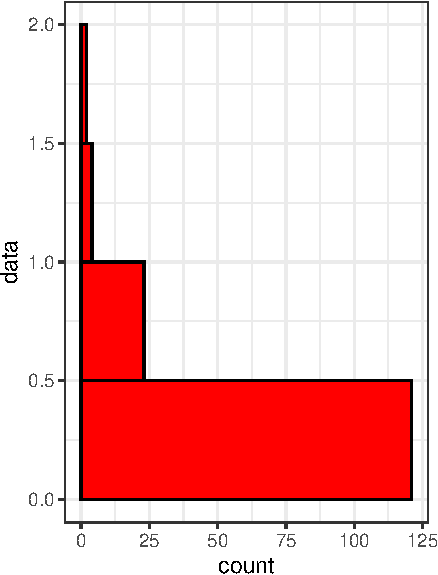
\includegraphics{BOAST_style_guide_files/figure-latex/skewEx1-1.pdf} 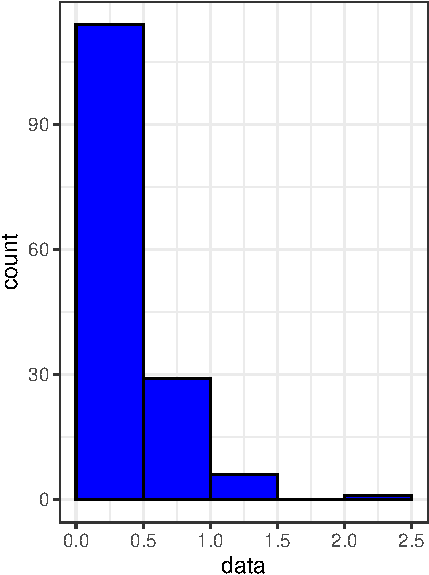
\includegraphics{BOAST_style_guide_files/figure-latex/skewEx1-2.pdf}

\hypertarget{choosing-terms-jingle}{%
\subsubsection{Choosing Terms-Jingle}\label{choosing-terms-jingle}}

We will always use the statistical/probabilistic meaning for a term, never the colloquial/everyday/non-technical meaning(s).

\hypertarget{option-2-entry-on-the-prerequisites-tabpage}{%
\subsection{Option 2: Entry on the Prerequisites Tab/Page}\label{option-2-entry-on-the-prerequisites-tabpage}}

Another option that you could do for both the jingle and jangle problems is to add an entry on the Prerequisites page. If you only have a jangle problem, you can use the \protect\hyperlink{hovertext}{Hover Text} option.

Option 2 can be combined with Option 1.

\hypertarget{footnotes}{%
\section{Footnotes}\label{footnotes}}

We recommend avoiding footnotes in favor of \protect\hyperlink{hovertext}{Hover Text}.

\hypertarget{documentation}{%
\chapter{Documentation}\label{documentation}}

These apps are the product of your hard work and are part of your academic record. Thus, you need to adhere to \href{https://undergrad.psu.edu/aappm/G-9-academic-integrity.html}{Penn State's Academic Integrity Policy}. This is especially important as we are making the apps available through a Creative Commons Attribution-ShareAlike 4.0 International license (\href{https://creativecommons.org/licenses/by-sa/4.0/}{CC BY-SA 4.0}). If you have used code, pictures, data, or other materials from outside of the BOAST team, you \textbf{MUST} give proper credit. These references will then be included on the App's References Tab.

\hypertarget{references-1}{%
\section{References}\label{references-1}}

All apps will need a References Tab. This is where you'll place all references for your App, including R packages, borrowed code, data sources, images, etc. This in addition to the Acknowledgments.

\textbf{NOTE:} listing something in the Acknowledgments DOES NOT waive this requirement.

You may use any citation style you wish, but be consistent. Recommended citation styles include APA and AmStat. Here is a starting code block for you to use:

\begin{Shaded}
\begin{Highlighting}[]
\CommentTok{#[omitted code]}
\KeywordTok{tabItem}\NormalTok{(}
  \DataTypeTok{tabName =} \StringTok{"refs"}\NormalTok{,}
  \KeywordTok{withMathJax}\NormalTok{(),}
  \KeywordTok{h2}\NormalTok{(}\StringTok{"References"}\NormalTok{),}
  \KeywordTok{p}\NormalTok{(}\DataTypeTok{class =} \StringTok{"hangingindent"}\NormalTok{,}
    \StringTok{"reference 1-alphabetically"}\NormalTok{),}
  \KeywordTok{p}\NormalTok{(}\DataTypeTok{class =} \StringTok{"hangingindent"}\NormalTok{,}
    \StringTok{"reference 2-alphabetically"}\NormalTok{),}
  \CommentTok{# Repeat as needed}
\NormalTok{)}
\end{Highlighting}
\end{Shaded}

Notice the use of \texttt{class\ =\ "hangingindent"}. You must include this with each reference as this will ensure the proper styling of your references.

If you need assistance with this section, please talk to Neil.

\hypertarget{plagiarism}{%
\section{Plagiarism}\label{plagiarism}}

\textbf{You MAY NOT use blocks of code you've found online without giving proper attribution.}

There is a difference between looking at example code online to see how to do something and copying that code directly. The former is permissible, the later is plagiarism.

\begin{itemize}
\tightlist
\item
  If you want to use someone else's code ``as is'' (without any changes), you should reach out to the author for permission first.
\item
  If you use someone else's code and make modifications, you need to give credit to where you got the code, and potentially ask for permission.
\end{itemize}

You will need to place citations in \emph{\textbf{two}} places: in the References Tab and in your code. You might want to also consider adding an acknowledgement to the Overview tab.

\hypertarget{reference-tab}{%
\subsection{Reference Tab}\label{reference-tab}}

Use the following format:

\begin{quote}
Author. (Date). Title of program/source code (Version number, if applicable). {[}type of code{]}. Retrieved from \textless{} URL \textgreater.
\end{quote}

For example,

\begin{quote}
Hatfield, N. J. (2017). First day activity (v1). {[}Netlogo{]}. Retrieved from \url{https://neilhatfield.github.io/statApps/Day1Activity.html}.
\end{quote}

\hypertarget{in-code}{%
\subsection{In Code}\label{in-code}}

Use the following format in your code to cite where you got the code from.

\begin{Shaded}
\begin{Highlighting}[]
\CommentTok{#-------------------------------------------------------------------------------}
\CommentTok{#  Title: <title of program/source code>}
\CommentTok{#  Author: <author(s) names>}
\CommentTok{#  Date: <date>}
\CommentTok{#  Code version: <code version>}
\CommentTok{#  Availability: <where it's located>}
\CommentTok{#-------------------------------------------------------------------------------}
\CommentTok{# [borrowed code then follows]}
\CommentTok{# ...}
\CommentTok{# [last line of borrowed code]      }
\CommentTok{#End of <author>'s code----------------------------------------------------------}
\end{Highlighting}
\end{Shaded}

\hypertarget{r-packages}{%
\section{\texorpdfstring{\texttt{R} Packages}{R Packages}}\label{r-packages}}

If you made use of any packages in \texttt{R}, then you will need to add these to the Reference tab. Fortunately, there is a built-in tool that will help you: the \texttt{citation} function. In R (RStudio) simply type \texttt{citation("packageName")} and you'll get the appropriate citation information for the package you used. For example, \texttt{citation("shinydashboard")} and \texttt{citation("plyr")} will give the information needed for the following citations:

\begin{quote}
Chang, W. and Borges Ribeio, B. (2018). shinydashboard: Create dashboards with `Shiny'. (v0.7.1) {[}R Package{]}. Available from \url{https://CRAN.R-project.org/package=shinydashboard}
\end{quote}

\begin{quote}
Wickham, H. (2011). The Split-apply-combine strategy for data analysis. Journal of Statistical Software, 40(1). pp.~1-29. Available at \url{http://www.jstatsoft.org/v40/i01/}.
\end{quote}

Notice, that the format of the R package will depend on whether there is an article published for the package. The \texttt{shinydashboard} package is not associated with an article while the \texttt{plyr} package is associated with Wickham's article.

\hypertarget{graphics-1}{%
\section{Graphics}\label{graphics-1}}

Pictures, drawings, photographs, images, etc. are typically copyrighted. When you're selecting images, make sure that the images are Open Source/Copyright Free/Royalty Free/Public Domain. Additionally, include a reference to where the pictures came from in the Overview Page. The basic format to use is:

\begin{quote}
LastName, First Initial. (Year). Title of artwork. {[}Format{]}. Retrieved from \textless{} URL \textgreater.
\end{quote}

\hypertarget{data}{%
\section{Data}\label{data}}

If you are using any data files, you need to attribute where those files are coming from in the References tab. You might also want to add an acknowledgement on the Overview tab. A suggested format to use is:

\begin{quote}
Author/Rightsholder. (Year). Title of data set (Version number) {[}Description of form{]}. Location: Name of producer.
\end{quote}

\begin{quote}
Author/Rightsholder. (Year). Title of data set (Version number) {[}Description of form{]}. Retrieved from \url{http://www.url.com}
\end{quote}

If you (or someone else) had to sign some type of agreement to access the data, we must examine the agreement before you make your App publicly accessible. Just because you got access to the data does not mean you have the right to share the data.

\hypertarget{part-accessibility-and-mobile-devices}{%
\part{Accessibility and Mobile Devices}\label{part-accessibility-and-mobile-devices}}

\hypertarget{accessibility}{%
\chapter{Accessibility}\label{accessibility}}

We need to make sure that our Apps are accessible. If you have been adhering to the style guide, your App should be in a decent position. When you're ready to test the accessibility of your App, you'll need to deploy the App to a sever and then use the \href{https://wave.webaim.org/}{WAVE Web Accessibility Evaluation Tool}. Enter the URL of your App in the noted box to run an evaluation. See what accessibility issues your App has and then address them.

\textbf{See also:}

\begin{itemize}
\tightlist
\item
  \href{https://accessibility.psu.edu/}{Accessibility and Usability at Penn
  State}
\item
  \href{https://www.psu.edu/accessibilitystatement}{Accessibility
  Statement}
\item
  \href{https://www.w3.org/WAI/WCAG21/quickref/}{How to Meet Web Content Accessibility
  Guidelines}
\item
  \href{https://medium.com/salesforce-ux/7-things-every-designer-needs-to-know-about-accessibility-64f105f0881b}{7 Things Every Designer Needs to Know about Accessibility}
\end{itemize}

\hypertarget{testing-accessibility}{%
\section{Testing Accessibility}\label{testing-accessibility}}

We highly recommend using the \href{https://wave.webaim.org/}{WAVE Web Accessibility Evaluation Tool}.

\begin{figure}

{\centering 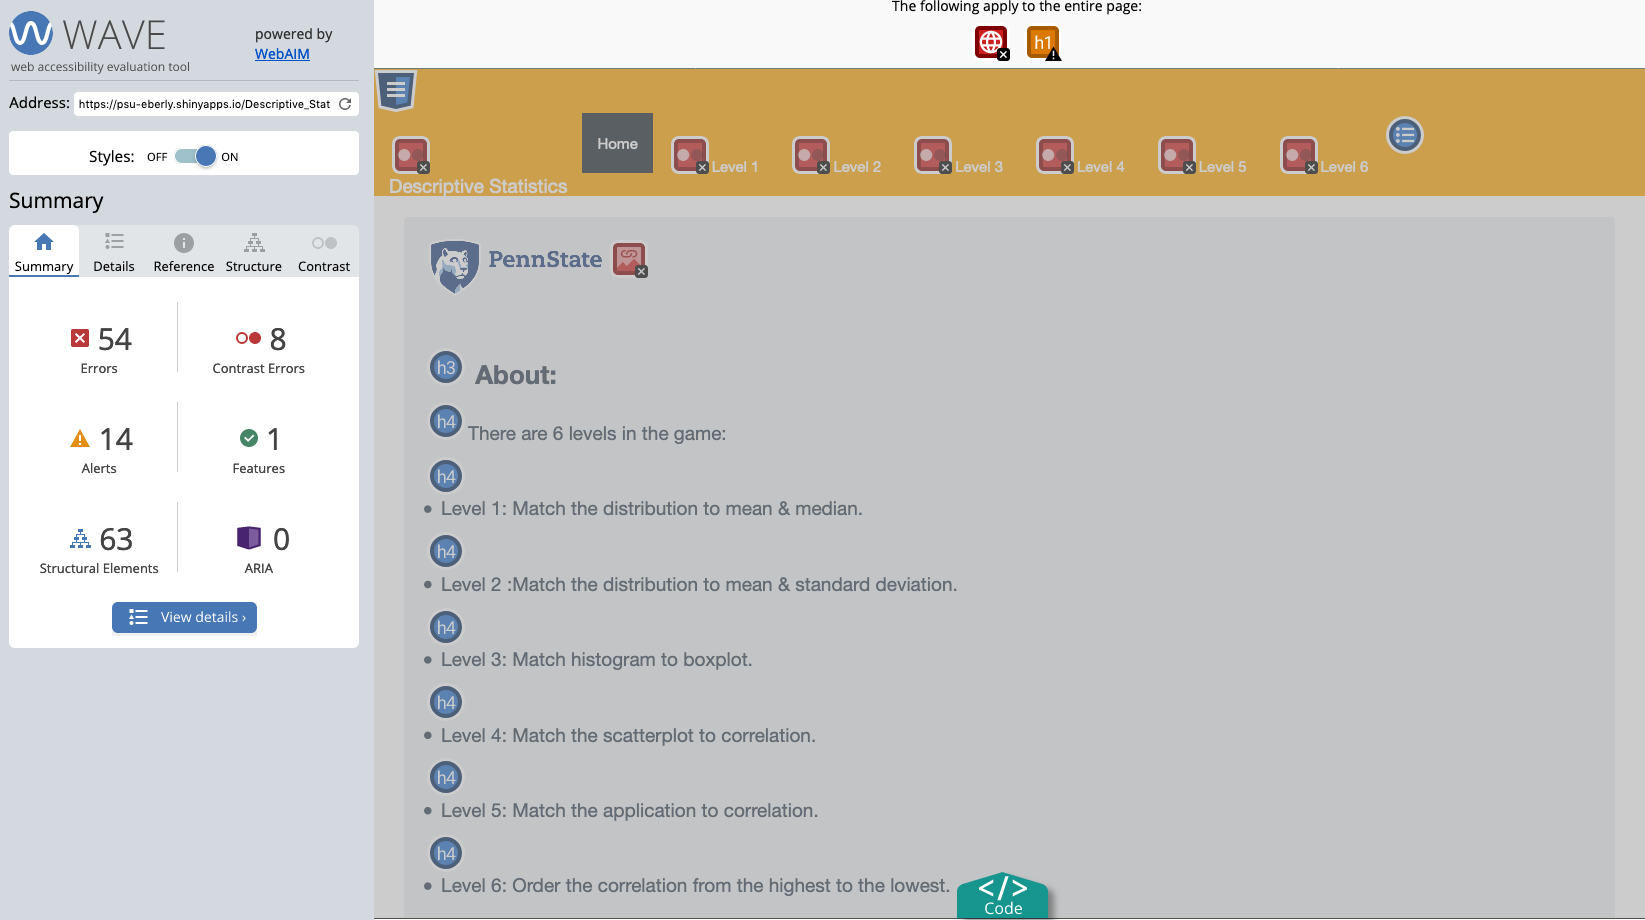
\includegraphics[width=22.85in]{images/descStatOverview} 

}

\caption{WAVE Report for Descriptive Statistics App}\label{fig:waveDescStat}
\end{figure}

Figure \ref{fig:waveDescStat} shows the WAVE report for the Descriptive Statistics App. There are 54 errors including missing alternative text, empty headings. There are also 8 contrast errors, 14 alerts (skipping heading levels),

\begin{figure}

{\centering 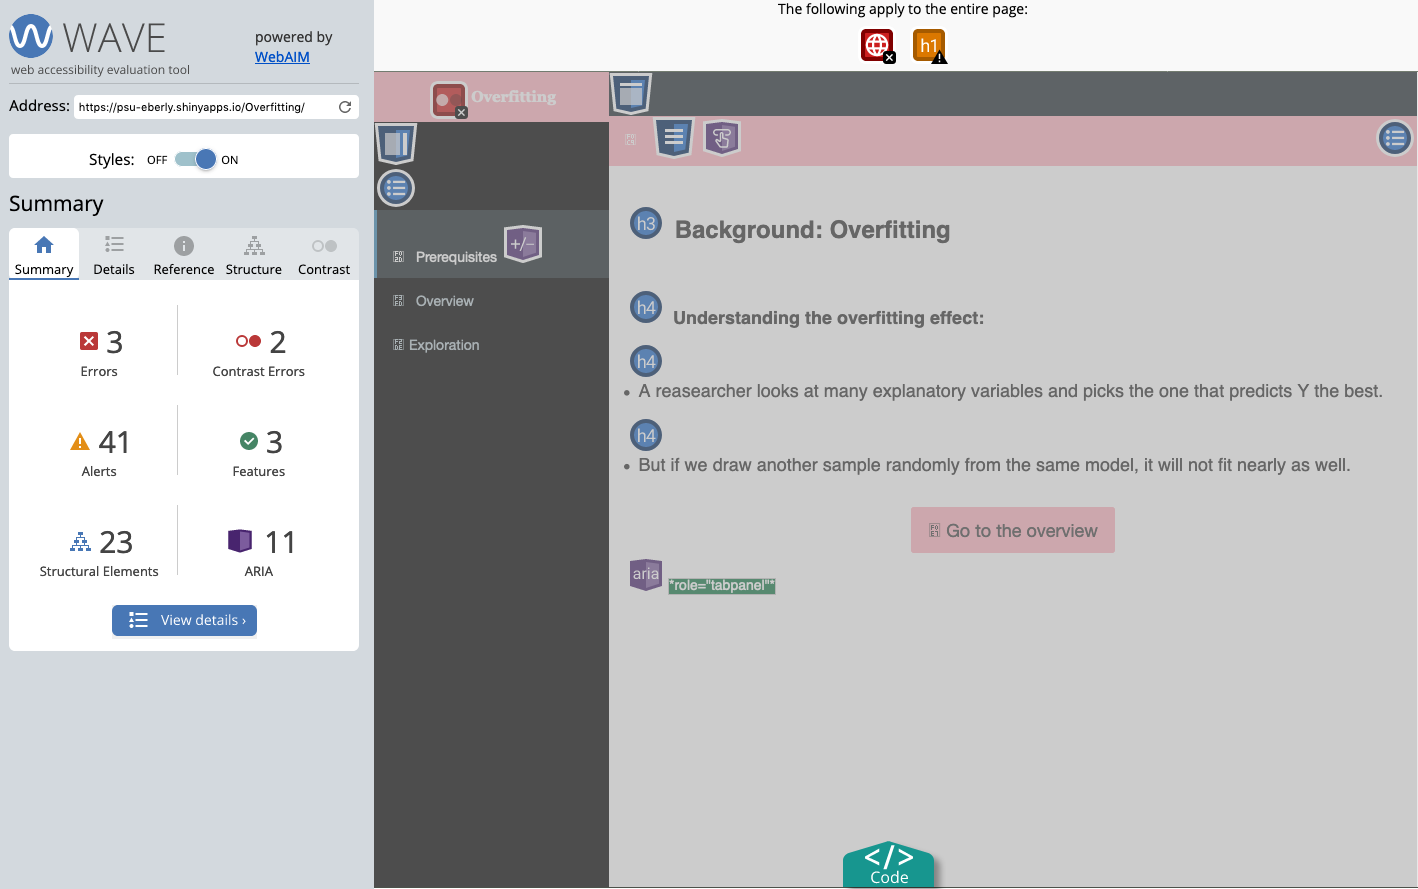
\includegraphics[width=19.69in]{images/overfitPrereq} 

}

\caption{WAVE Report for Overfitting App}\label{fig:waveOverfit}
\end{figure}

While there are fewer errors for the Overfitting App (Figure \ref{fig:waveOverfit}), there are a lot of alerts on this app including skipping heading levels and small text.

By using the \texttt{boastApp} function and adhering to this Style Guide, your App should be in a good initial position. After running your App through WAVE, we can work with you address any changes that might be necessary.

\hypertarget{mobile}{%
\chapter{Mobile Friendliness}\label{mobile}}

We want our apps to work well with mobile devices. Thus, when you get to the point where the majority of bugs have been fixed, you need to check how mobile friendly your App is. If you have used \texttt{boastApp} and/or the \texttt{boast.CSS} file, along with the practices laid out earlier, then you should be well on your way to being mobile friendly.

You can check your App in two ways:

\begin{enumerate}
\def\labelenumi{\arabic{enumi}.}
\tightlist
\item
  Test your App out on a variety of mobile devices.
\item
  Make use of a browser's ability to mimic devices. To do this, launch your App in a browser, then enable one of the following:

  \begin{itemize}
  \tightlist
  \item
    \href{https://developers.google.com/web/tools/chrome-devtools/device-mode/\#viewport}{Chrome: Device Mode}
  \item
    \href{https://developer.mozilla.org/en-US/docs/Tools/Responsive_Design_Mode}{Firefox: Responsive Design Mode}
  \item
    \href{https://docs.microsoft.com/en-us/microsoft-edge/devtools-guide/emulation}{Microsoft Edge: Device Emulation}
  \item
    \href{https://support.apple.com/en-gb/guide/safari-developer/dev84bd42758/mac}{Safari: Responsive Design Mode}
  \end{itemize}
\end{enumerate}

Look for any issues that you might be able to address before you hand off your App for others to play around with. Assign a \textbf{Mobile Friendliness Rating} to your App on a scale from 1 to 5.

\begin{enumerate}
\def\labelenumi{\arabic{enumi}.}
\tightlist
\item
  Not functional
\item
  Functional -- Very awkward
\item
  Functional -- Okay if no big screen available (multiple issues)
\item
  Usable in a small class setting (single issue)
\item
  Readily usable
\end{enumerate}

\hypertarget{part-examples}{%
\part{Examples}\label{part-examples}}

\hypertarget{makingApp}{%
\chapter{Making an App}\label{makingApp}}

Sooner or later, you'll reach the point where it is time to make your own Shiny App for BOAST. Approaching your App's construction in a systematic way will help you tremendously. The following suggested workflow is an abbreviated version of the one in Section \ref{workflow}:

\begin{enumerate}
\def\labelenumi{\arabic{enumi}.}
\tightlist
\item
  Read the Style Guide
\item
  Identify a topic
\item
  Sketch out your plans
\item
  Create a new repository on GitHub
\item
  Begin writing the code
\item
  Edit and locally Test your code
\item
  Push your code to GitHub/Create a dev branch
\item
  Push your edits
\item
  Larger scale testing
\item
  Pull Request
\item
  Additional tweaks
\end{enumerate}

This workflow (both in the more expanded state and in the abbreviated one) leaves out a lot of the going-ons and decision making that goes into making an app. Our goal with this section is to walk you through this process as Neil makes an app from scratch.

\hypertarget{step1}{%
\section{Step 1: Read the Style Guide}\label{step1}}

This is step is critical to making an app that is easy to debug (vital when programming) and is in-alignment with the Standards that we have set for BOAST. Please take your time going through the Style Guide and keep an eye on it for updates. You can access the published Bookdown version by clicking on the address link located at the top of the Guide's GitHub Repository.

As you build your App, we recommend periodically checking the Style Guide to 1) ensure that you're still adhering to it, 2) to stay up-to-date with the Guide, and 3) to see (and then use) any useful code chunks that are listed. Even as the authors of this Guide, we're constantly looking things up. Thus, there is no shame in constantly referring to the Style Guide; after all, it is meant to be a Go-To Reference.

\hypertarget{step2}{%
\section{Step 2: Identify a Topic}\label{step2}}

This is one of the more challenging tasks for anyone: deciding what to make an app about. The notion of ``picking a topic'' is a bit misleading as not only should you pick a topic, but you also need to pick the purpose of the app, and the goals. While all three go hand-in-hand with each other, the easiest decision of the three is purpose.

\hypertarget{step2a}{%
\subsection{Your App's Purpose}\label{step2a}}

When we look across BOAST, we can categorize the apps into two major classes: apps whose purpose is to help students \textbf{learn} an idea/concept and apps whose purpose is to help students \textbf{review} an idea/concept. The \href{https://psu-eberly.shinyapps.io/Significance_Testing_Caveats/}{NHST Caveats App} stands as a good example of an app whose purpose is to help students learn something. On the other hand, the \href{https://psu-eberly.shinyapps.io/Hypothesis_Testing_Game/}{{[}Null{]} Hypothesis Testing Game (Tic-tac-toe)} and the \href{https://psu-eberly.shinyapps.io/Matching_Distributions/}{Matching Distributions} are examples where the student is reviewing their understandings. There are some apps such as \href{https://psu-eberly.shinyapps.io/ANCOVA/}{ANCOVA} that are dual purpose, having both learning elements and reviewing elements.

Generally speaking, apps whose purpose is \textbf{learning} are going have Explorations and possibly Challenges for Activity Tabs. Apps whose purpose is \textbf{reviewing} will have just Games for Activity Tab(s).

By identifying early on the purpose of your App, you'll be able to better plan your app.

\hypertarget{step2b}{%
\subsection{The Topic}\label{step2b}}

Here is where you'll decide what statistical idea/concept your App is going to be centered around. While you should be as specific as possible here, \textbf{apps for learning} need to have much more specificity than \textbf{apps for reviewing}. Saying that you want your App ``to deal with probability'' is not going to be as useful as saying that you want your App ``to help students recognize when probability is and is not appropriate for different contexts''.

Don't feel like you have to details to the nanoscale. As you continue developing and talking with people, you'll start adding in more details.

You can identify potential topics through any of the following:

\begin{itemize}
\tightlist
\item
  Think of a concept in a Stat class that you (or your peers) struggled with (or still do)
\item
  Think of a concept where you thought to yourself ``I wish there was a way to visualize this''
\item
  Think of a concept where you went ``How does this work?''
\item
  Did you see/hear about a new study and thought to yourself ``what's going on?''
\item
  Did a media report make you do a double take?
\item
  Ever think to yourself ``I wish I had more practice with {[}topic{]}.''
\item
  And more
\end{itemize}

Again, this list is just a starting place to identify potential topics. Draw inspiration from your experiences, your curiosity. Bounce ideas off of each other and the faculty.

\emph{\textbf{Word of Caution \#1}}: While it is okay to get ideas from other websites, please keep track of this. We need to give credit where credit is due. If you come across an app (whether in Shiny or some other program) somewhere and you think that it would be good to translate that into Shiny app for BOAST, we need to know.

\emph{\textbf{Word of Caution \#2}}: An unproductive place to begin is to say ``Hey, I want to make a memory game'' or ``I saw this really cool animation and I want to make an app that does that.'' Both of these (especially the second) place the educational aspect of the app as a secondary focus. \textbf{This is not consistent with BOAST.} All apps should place educational purposes and goals before anything else. Forcing a topic to make use of certain tool because that tool would be ``cool'' or ``fun'' does not further our goals. We should strive for synergy between topics and the tools within Shiny.

\hypertarget{step2c}{%
\subsection{Goals}\label{step2c}}

Now, we're sure that some people have already thought to themselves ``hey, you've already had us identify purpose so isn't this the same?'' To which we reply ``No.'' We've used \textbf{purpose} to refer an overarching aim of your App. Here, \textbf{goal} refers to a much more contextualized aspect. While these goals will be less important for reviewing apps, you will need to identify specific learning goals for learning apps.

For this step, you're going to need to work with the faculty to identify the learning goals for your app. If you're drawing from a past experience in a course, look to see if there were learning objectives listed. Those can be extremely useful starting places.

\hypertarget{example}{%
\subsection{Example}\label{example}}

\emph{The following is a somewhat stream-of-consciousness narrative of how Neil tackled this step. We'll place flags in parentheses.}

I would like to make an app that would help introductory students (\emph{identifies an intended audience}) wrestling with some of the concepts of descriptive/incisive statistics (\emph{Purpose: learning}). Some ideas that I have are:

\begin{itemize}
\tightlist
\item
  Conceptualizing the two distinct uses of the \emph{sample arithmetic mean}--mitigation of measurement errors of a single object vs.~measuring how well a group of objects/beings performs
\item
  Conceptualizing statistics as functions that measure attributes of collections
\item
  Conceptualizing the relationship between the values of the \emph{sample median} and \emph{sample arithmetic mean} is not a competition (i.e., one is not ``better than'' the other)
\item
  Avoid falling into the skewness trap for the ordering of the values of the \emph{sample median} and \emph{sample arithmetic mean}.
\end{itemize}

This last option feels like a fairly straightforward (and simple) app to create. Additionally, there's an \href{http://jse.amstat.org/v13n2/vonhippel.html}{article by von Hippel on this issue} I can reference. (\emph{Topic: relationship between the values of }sample median \emph{and} sample arithmetic mean \emph{in the presence of skewness})

After using the app, a student should recognize that while for a many data collections that have skewness, the value of the \emph{sample arithmetic mean} will be either greater (for positive skew) or less (for negative skew) than the value of the \emph{sample median}, this is not an absolute rule. (\emph{Learning Goal})

\hypertarget{step3}{%
\section{Step 3: Sketch out plans}\label{step3}}

Something to keep in mind with this workflow is that it is not strictly linear. That is, just because you have moved into Step 3, doesn't mean that you can't go back to Step 2 and make revisions. Additionally, as you get into Steps 5-8, you might find yourself coming back to Step 3 (and possibly Step 2) and making changes. This said, sketching out your plans will help you as you move forward with developing.

There are several things that you'll want to be sure that you include in your sketch:

\begin{itemize}
\tightlist
\item
  A Suggested Title

  \begin{itemize}
  \tightlist
  \item
    This might not be what you settle on, but you'll need to have this firmed up by the time you get to Step 4.
  \item
    You'll want to have both a {[}Long/Formal{]} Name and a shortened name ready
  \end{itemize}
\item
  Goal(s) of the App

  \begin{itemize}
  \tightlist
  \item
    Carry this forward from Step 2 as a tangible reminder
  \item
    If you have several goals, you might consider denoting which tabs go with which goals
  \end{itemize}
\item
  What will the user be doing

  \begin{itemize}
  \tightlist
  \item
    Thinking about what you want the user to do
  \item
    Identify anything the user might click on, drag, or otherwise manipulate.
  \item
    If there are going to be options, identify what those options should be.
  \item
    Will there be different levels?
  \item
    Will there be a Challenge tab?
  \end{itemize}
\item
  What will the user experience

  \begin{itemize}
  \tightlist
  \item
    Think about the general layout (explore, game, etc.)
  \item
    What outputs should the user be examining
  \end{itemize}
\item
  What are the relationships between elements

  \begin{itemize}
  \tightlist
  \item
    Think about how each input impacts the outputs
  \item
    If you want the user to have a certain experience, does the coding allow for that experience to happen?
  \end{itemize}
\item
  Other Elements

  \begin{itemize}
  \tightlist
  \item
    Are you going to reference any external images?
  \item
    Are you going to import any data files? If so, which ones? Do you have them?
  \item
    Is there an activity packet?
  \end{itemize}
\end{itemize}

The format of your sketches is up to you.

\hypertarget{example-1}{%
\subsection{Example}\label{example-1}}

As I start thinking about what this app might look like, I'm going to use a sheet of paper in quarters to organize some thoughts. Figure \ref{fig:planSketchFull} shows the entire sheet of paper. The quadrants move left to right, top to bottom.

\begin{figure}

{\centering 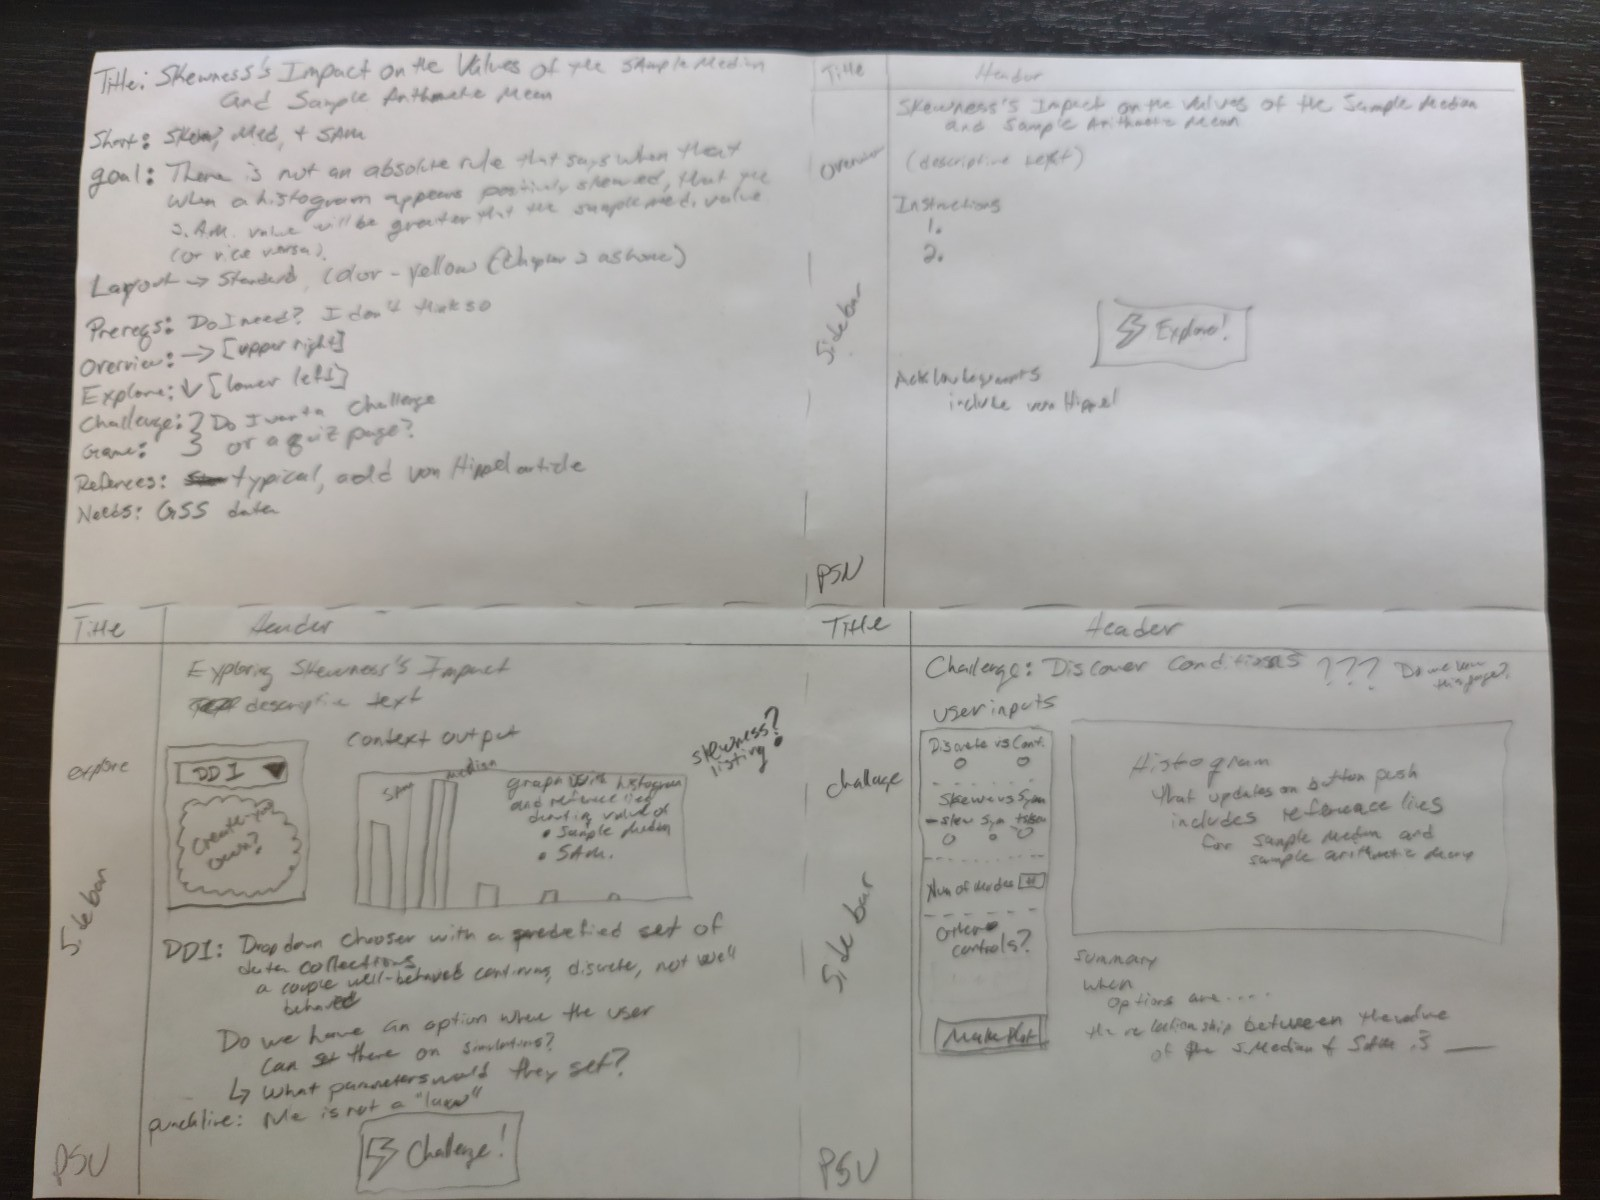
\includegraphics[width=22.22in]{images/planSketch1} 

}

\caption{Picture of My Plan}\label{fig:planSketchFull}
\end{figure}

In the first quadrant (Figure \ref{fig:planSketchInfo}), I've listed a title (``Skewness's Impact on the Values of the \emph{Sample Median} and \emph{Sample Arithmetic Mean}''), a possible short title (``Skew, Med, SAM'') as well as a restatement of my goal. I've then listed general aspects about the layout of my app, including what skin/theme color (yellow) I would need to use.

I've additionally identified that I need to include the von Hippel article in my Reference Tab as well as locating a version of the General Social Survey (GSS).

\begin{figure}

{\centering 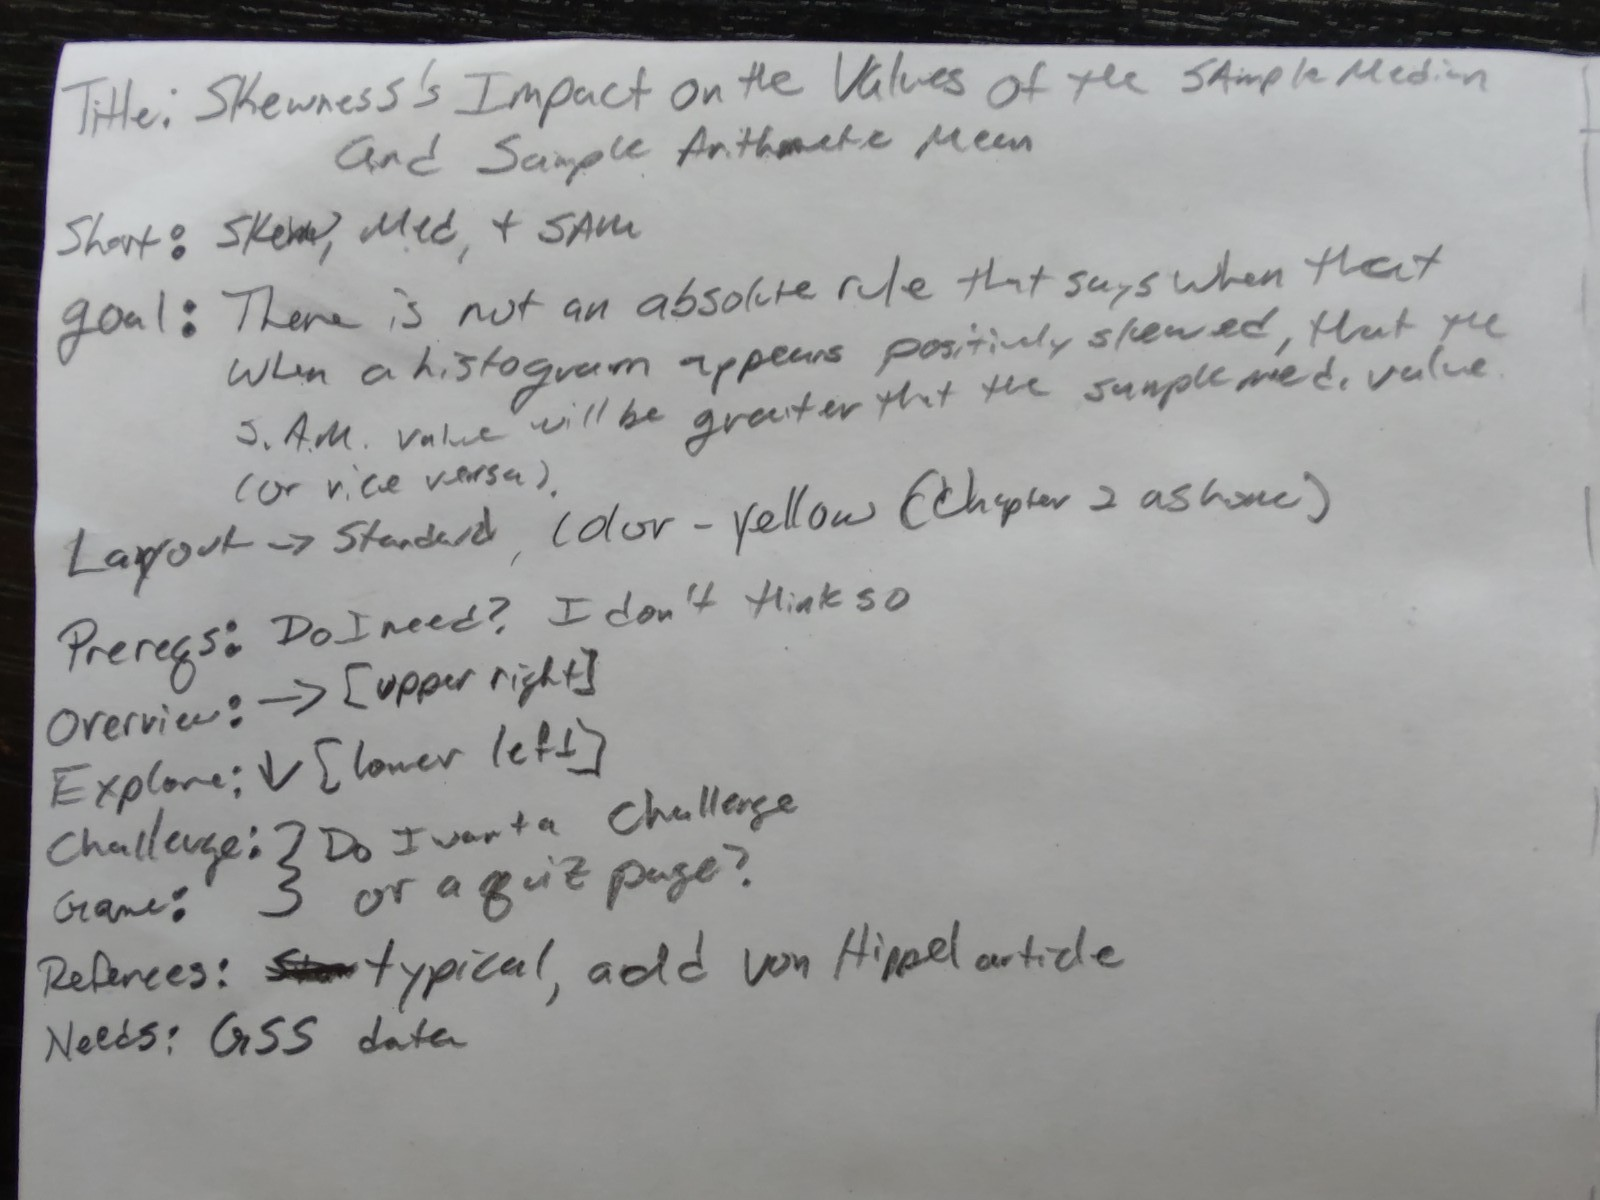
\includegraphics[width=22.22in]{images/planSketch2-Info} 

}

\caption{First Quadrant: General Information}\label{fig:planSketchInfo}
\end{figure}

The second quadrant of my paper is the Overview Tab sketch (Figure \ref{fig:planSketchOverview}. I don't have much information here.

\begin{figure}

{\centering 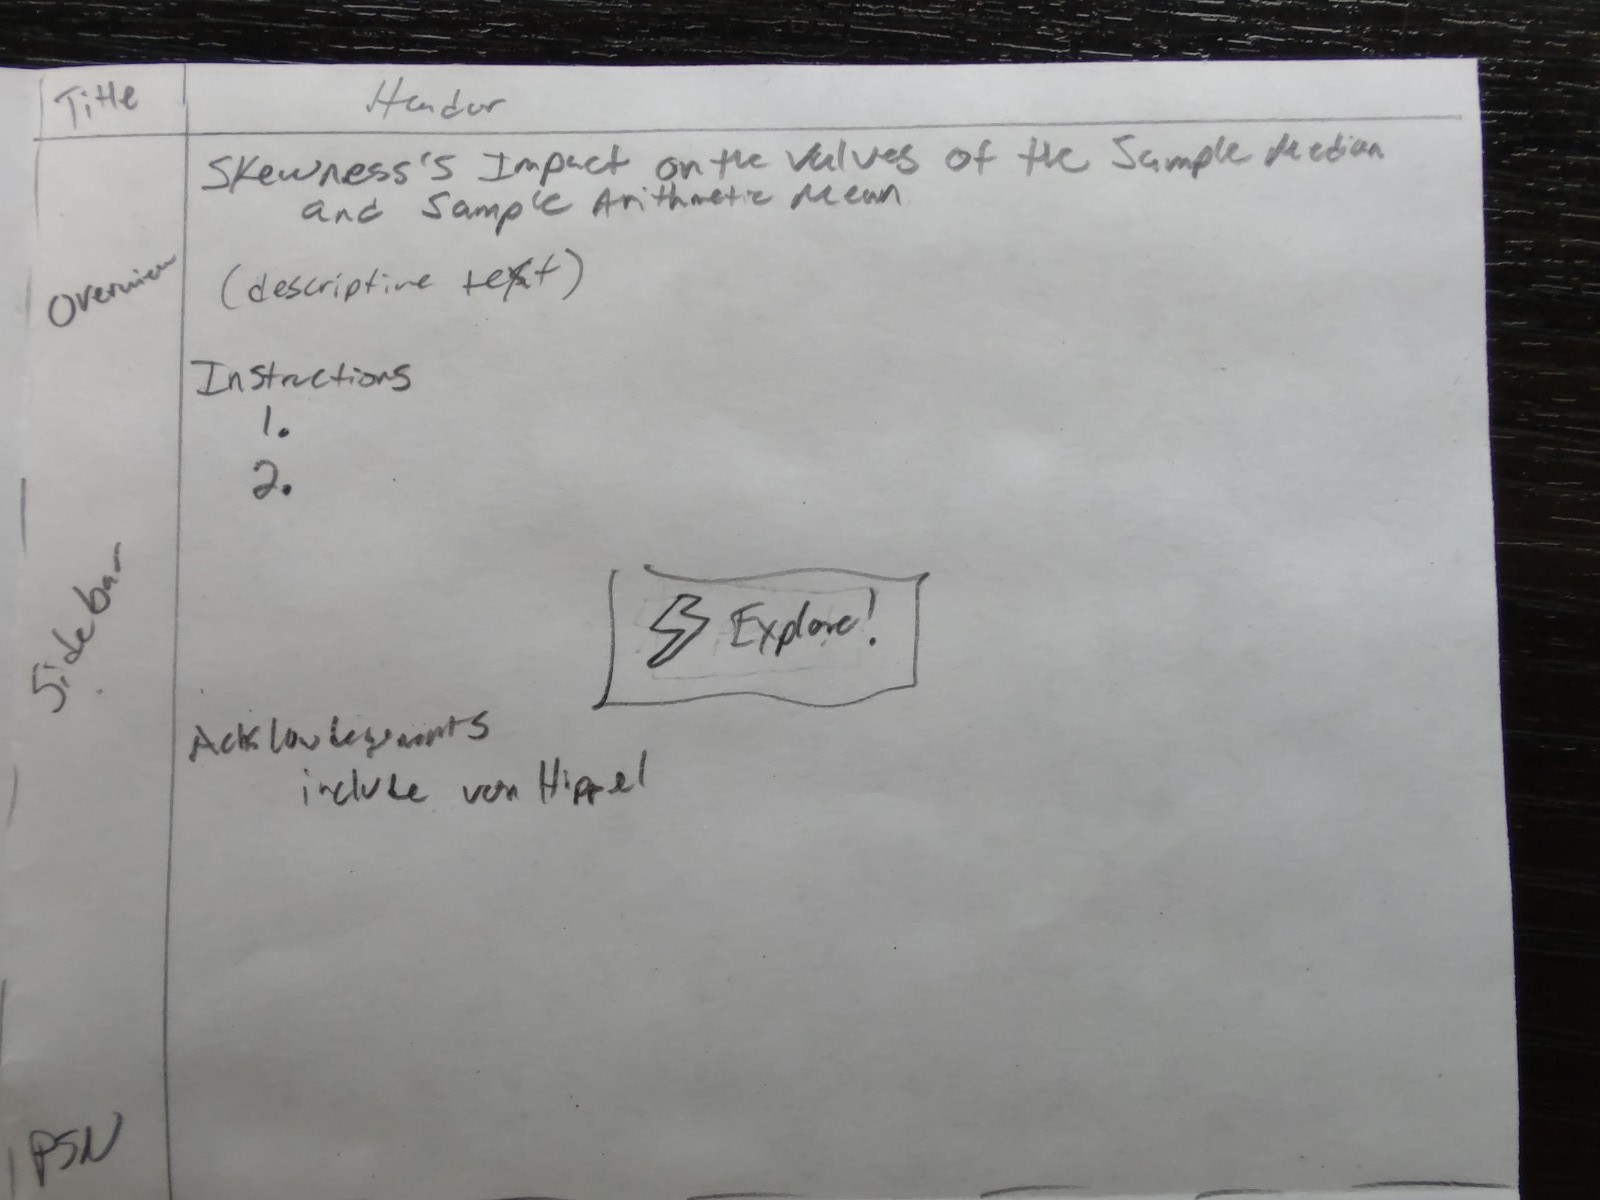
\includegraphics[width=22.22in]{images/planSketch3-Overview} 

}

\caption{Second Quadrant: Overview Tab}\label{fig:planSketchOverview}
\end{figure}

\begin{figure}

{\centering 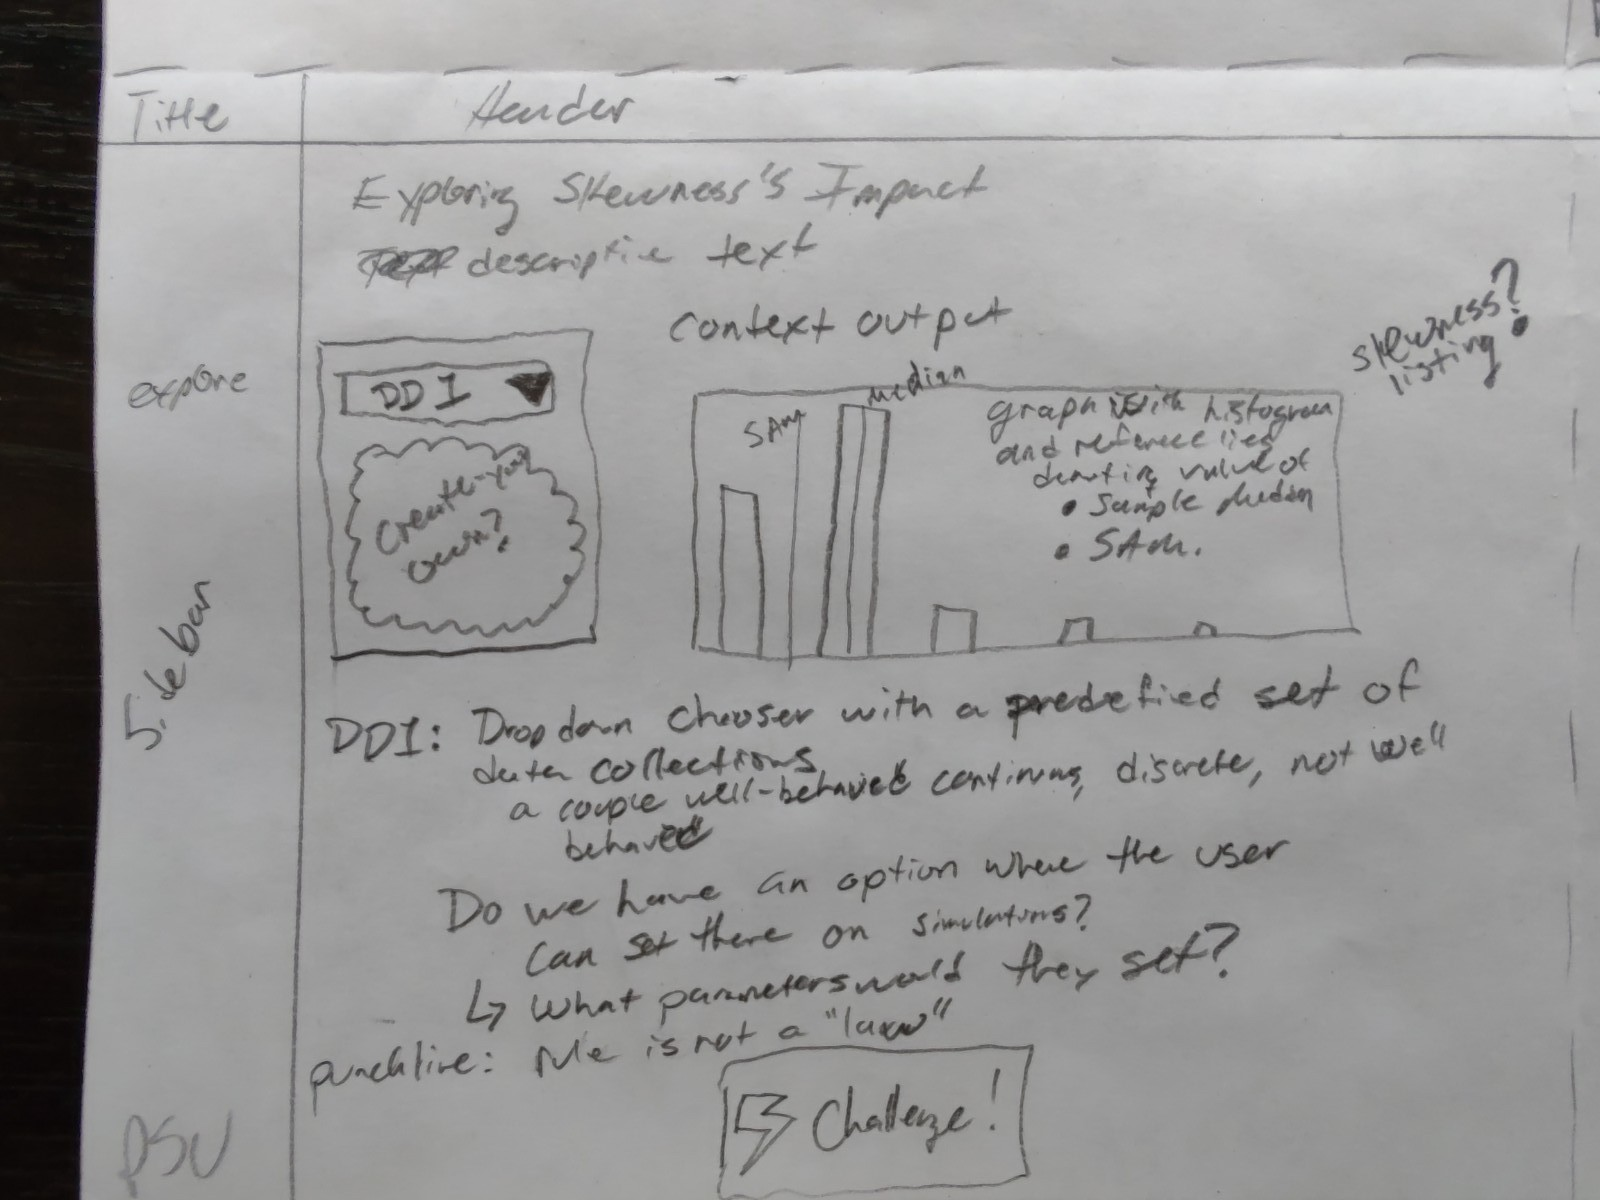
\includegraphics[width=22.22in]{images/planSketch4-Explore} 

}

\caption{Third Quadrant: Exploration Tab}\label{fig:planSketchExplore}
\end{figure}

The next quadrant (Figure \ref{fig:planSketchExplore}) is where I started detailing the first Activity Tab of my app: the first Exploration. I'm imagining that in this exploration that the user would look through a variety of cases where the ``rule'' does and does not work. What I want the user to walk away from this tab is that just because a histogram looks positively skewed does not imply that the value of the \emph{sample arithmetic mean} is greater than the value of the \emph{sample median}.

I'm imagining a drop-down menu that would allow the user to move through a variety of data sets. Ideally, these data sets would be real data. The General Social Survey, has a variety of attributes that we could use, include several that demonstrate what I want. For example, the number of adults (18+ y.o.) living in a household is positively skewed but the value of the \emph{sample median} is larger than than the value of the \emph{sample arithmetic mean}. Which each choice of the user makes, the histogram on the right will update to show the appropriate data, plus reference lines for the values of the two statistics. I might want to add a numerical display as well. I also want there to be some context helping the user to understand each choice.

I've left as an open question whether to enable a user to import/create their own data set on this tab. I'm currently leaning towards not allowing this. Additionally, I've marked something for a punchline but this will need more thought.

\begin{figure}

{\centering 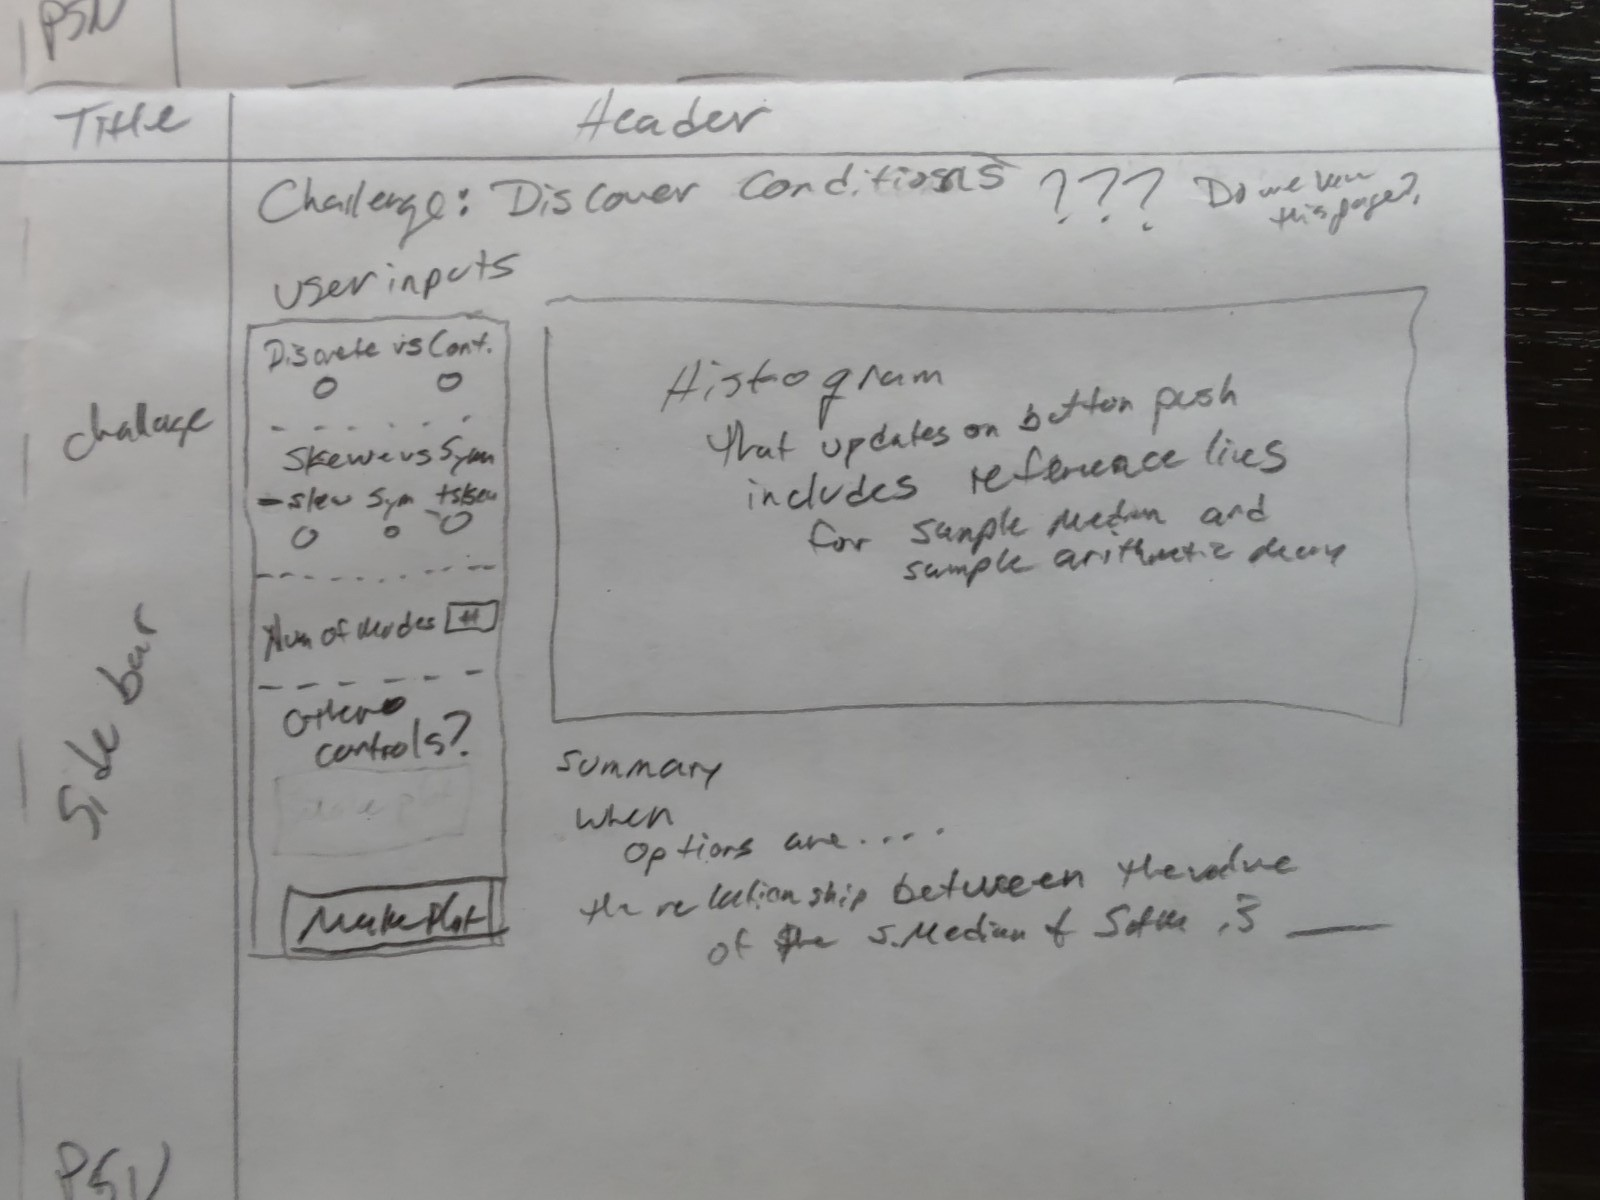
\includegraphics[width=22.22in]{images/planSketch5-Challenge} 

}

\caption{Fourth Quadrant: Challenge Tab}\label{fig:planSketchChallenge}
\end{figure}

The fourth and final quadrant (Figure \ref{fig:planSketchChallenge}) is an idea I'm still kicking around. This would depend on the specific audience and course goals for which users would go here. My idea is to extend the goal for the app to allow students to construct an understanding for what conditions might lead to \(Sample\;Median\left(\mathcal{X}\right)<SAM\left(\mathcal{X}\right)\), \(Sample\;Median\left(\mathcal{X}\right)=SAM\left(\mathcal{X}\right)\), and \(Sample\;Median\left(\mathcal{X}\right)>SAM\left(\mathcal{X}\right)\).

At this moment, I'm leaning towards marking the Challenge Tab as being a future improvement/addition rather than being part of the initial version of the app.

\hypertarget{share-your-plan}{%
\subsection{Share Your Plan}\label{share-your-plan}}

Once you have a sketch, you'll want to share this plan with others to get ideas for suggestions, modifications, etc. Different people might be able to point you to code snippets you can reuse from other apps. More importantly, they might be able to help you think about things that you glossed over/missed and/or thought about but didn't articulate. By sharing these plans, we'll make better apps.

This is also the point in time in which the faculty will say whether you can go ahead and move to Step 4.

\hypertarget{step4}{%
\section{Step 4: Create Repository}\label{step4}}

Here you'll want to reference Section \ref{repo-naming} on GitHub Repo Naming. Most app {[}full{]} titles don't make good Repo Names. This is where the potential short title comes into play. You'll need to make sure that there isn't already a repository that has that name. When you get a name figured out for the repository, you can go ahead and create the repo.

Make sure to set Git Ignore to \texttt{R}.

\hypertarget{steps5-8}{%
\section{Steps 5-8: Write, Edit, Test, Debug}\label{steps5-8}}

We recommend starting with a copy of the Sample App as the basis. This will give you a good skeleton to use for your new app.

(\emph{Still under construction})

\hypertarget{step9}{%
\section{Step 9: Larger Scale Testing}\label{step9}}

(\emph{Still under construction})

\hypertarget{steps10-11}{%
\section{Steps 10-11: Pull Requestion and Tweaks}\label{steps10-11}}

(\emph{Still under construction})

\hypertarget{part-final-thoughts}{%
\part{Final Thoughts}\label{part-final-thoughts}}

\hypertarget{addTools}{%
\chapter{Additional Tools}\label{addTools}}

Here are a few additional tools that can help you with App development:

\begin{itemize}
\tightlist
\item
  \href{https://github.com/jimhester/lintr}{lintr} - Checks adherence to a
  given style, syntax errors, and possible semantic issues.
\item
  \href{https://www.tidyverse.org/articles/2017/12/styler-1.0.0/}{styler} -
  Format R code according to a style guide.
\item
  \href{https://github.com/MichaelChirico/funchir}{funchir} - stale package
  check
\end{itemize}

\textbf{R Code}

\begin{Shaded}
\begin{Highlighting}[]
\KeywordTok{install.packages}\NormalTok{(}\KeywordTok{c}\NormalTok{(}\StringTok{"funchir"}\NormalTok{, }\StringTok{"lintr"}\NormalTok{, }\StringTok{"styler"}\NormalTok{))}
\end{Highlighting}
\end{Shaded}

  \bibliography{book.bib,packages.bib}

\end{document}
